% Gelfand seminar notes, 1973-74: source pages P000501-P000553.
% Russian diplomatic transcription (AI-made, checked against the scans), cut page by page from the cumulative working reader A4-reader-chapters01-32-opening-first1444-separated-diplomatic-r2.
% \SourcePage{GELFAND-Pnnnnnn}{label} starts a scanned page; the second argument is the number written
% on the page, if any. Editorial notes give the page, a label and the transcriber's remark; \Unclear
% marks a doubtful reading.
\SourcePage{GELFAND-P000501}{1}
\uuline{3/\mbox{\uuline{IX}}-73.}\qquad\uline{Сем.}
\Incomplete{GELFAND-P000501}{heading-cancelled}{Текст между «Сем.» и «Гельфанда» густо зачёркнут. Чтение не установлено.}
\end{GelfandAdjacentEvidence}
\begin{GelfandAdjacentEvidence}{GELFAND-P000501}{2}

\uline{Гельфанда.}

\uuline{План}:

1. Производная категория (Кириллов, Бернштейн).

2. Теория Алфорса — Неванлинна для многих переменных (и Грауэрту). (Хенкин, Шабат).

3. $K$-теория (симплициальный вариант) по Quillen'у (Фукс).
\Unclear{GELFAND-P000501}{plan-k-theory}{Бледные слова условно прочитаны как «симплициальный вариант».}
\end{GelfandAdjacentEvidence}
\begin{GelfandAdjacentEvidence}{GELFAND-P000501}{3}


4. Гипотеза Лихтенбаума о связи между $\zeta$-ф-ей в целых точках и высшими $K$-теориями (Манин).

5. Вей: идеология Герстенцуса.
\Unclear{GELFAND-P000501}{plan-item-five}{Фамилия условно прочитана как «Герстенцуса».}
\end{GelfandAdjacentEvidence}
\begin{GelfandAdjacentEvidence}{GELFAND-P000501}{4}


\uline{Интермедия}:
\Unclear{GELFAND-P000501}{interlude-number}{Слева густо наведён номер. Возможно 6 или 8.}
\end{GelfandAdjacentEvidence}
\begin{GelfandAdjacentEvidence}{GELFAND-P000501}{5}

\uuline{2 проблемы Серра}:

1) $k[t]$, $k$ — конечно;
$SL_n(k[t])$, $n\geq 3$;
$SL_n(k[t,t^{-1}])$, $n\geq 2$

Эти группы имеют конечное число образующих. Являются ли они конечно представленными? (Сущ. ли образ., между котор. конечное число соотнош.).

2) Когер. группа: $\forall$ подгр. с кон. числом обр. конечно представлена.
Свободная и нильпот. когерентны.
\Unclear{GELFAND-P000501}{coherent-groups}{Бледное сокращение прочитано как «нильпот.».}
\end{GelfandAdjacentEvidence}
\begin{GelfandAdjacentEvidence}{GELFAND-P000501}{6}

Фунд. группы 3-мерных мн-зий когерентны
(G. P. Scott, J. Lond. Math. Soc., (2)6 (1973), 437--440). Статья.
$SL_2(\Lambda)$ когер., где $\Lambda$ — чисто мнимые элем. квадр. поля.
\Unclear{GELFAND-P000501}{lambda-description}{Бледная запись условно прочитана как «чисто мнимые элем. квадр. поля».}
\end{GelfandAdjacentEvidence}
\begin{GelfandAdjacentEvidence}{GELFAND-P000501}{7}

\Unclear{GELFAND-P000501}{lambda-cancelled}{Зачёркнутое слово условно читается как «ещё».}
\end{GelfandAdjacentEvidence}
\begin{GelfandAdjacentEvidence}{GELFAND-P000501}{8}


Явл. ли $SL_3(\mathbb Z)$ или $SL_2(\mathbb Z[\frac1p])$ когерентными?
$GL_n(\mathbb Q)$?

[много ли соотнош. между разл. неприводимыми? (кон. числом)]
\Unclear{GELFAND-P000501}{interlude-relations}{Бледное сокращение условно прочитано как «соотнош.».}
\end{GelfandAdjacentEvidence}
\begin{GelfandAdjacentEvidence}{GELFAND-P000501}{9}

\Unclear{GELFAND-P000501}{interlude-question}{Слово условно прочитано как «неприводимыми».}
\end{GelfandAdjacentEvidence}
\begin{GelfandAdjacentEvidence}{GELFAND-P000501}{10}


[Какие бывают фунд. группы?]

6. \uline{Смейл}: оптимизация нескольких функций.
\Unclear{GELFAND-P000501}{plan-six-overwriting}{Цифра густо наведена. Читается как 6 по очертаниям и соседней нумерации.}
\end{GelfandAdjacentEvidence}
\begin{GelfandAdjacentEvidence}{GELFAND-P000501}{11}


7. \uline{Браун, Дуглас, Филлмор} \quad Правильная $K$-теория от нескольких переменных (Кириллов).

8. \uuline{Мищенко}: представления в его смысле.

9. \uline{Люстиг}: высш. сигн. Новикова\qquad J. Diff. Geom. 197(1)
\Unclear{GELFAND-P000501}{novikov-name}{Бледная фамилия условно прочитана как «Люстиг».}
\end{GelfandAdjacentEvidence}
\begin{GelfandAdjacentEvidence}{GELFAND-P000501}{12}


10. \uline{Атья, Ботт, Патоди об \mbox{$L$}-функциях, связ. с ур-ями.}
(спектр. асимметр. и т. д.) (Шубин)

11. \uuline{Донован, Фрейлих} а (В. Пономарёв) — четвёрка подпр-в и т. д.
\Unclear{GELFAND-P000501}{plan-item-eleven-mark}{Небольшой знак условно прочитан как «а».}
\end{GelfandAdjacentEvidence}
\begin{GelfandAdjacentEvidence}{GELFAND-P000501}{13}

Модули и т. д.

12. Ю. И. Манин.

13. Вершик, Гельфанд, Граев — 6 вариаций на тему $SL_2$.

\uuline{Ю. И. Манин.}\qquad\uline{\mbox{$p$}-адические меры}

\uline{Сюжет}: $\mathbb Q_p$;\quad $K$ — конечн. расш.
$X$ — компактное $p$-ад. аналит. мн-зие над $K$.
Пример: целые числа в $K$, их прямые произв. и т. п.

\SourceFigure{GELFAND-P000501}{field-tower-and-maps}{Слева башня полей без стрелок. Рядом аналитическое отображение и пример координаты.\par\smallskip
{\centering
\begingroup\color{black}\GelfandFitDiagram{\begin{tikzpicture}
\node (L) at (0,1.50) {$L$};
\node (K) at (0,.75) {$K$};
\node (Q) at (0,0) {$\mathbb Q_p$};
\draw (L)--(K)--(Q);
\node (X) at (1.14,1.09) {$X$};
\node (cod) at (2.66,1.09) {$L$};
\draw[->] (X)--node[above] {$f$} node[below,font=\scriptsize] {аналит.} (cod);
\node[anchor=west,font=\scriptsize] at (3.12,1.45) {целые $A$};
\node[anchor=west,font=\scriptsize] at (3.12,.86) {\uline{Прим.}:};
\node (A) at (4.21,.86) {$A$};
\node (Ktwo) at (5.50,.86) {$K$};
\draw[->] (A)--node[above] {$x$} (Ktwo);
\node[anchor=west,font=\scriptsize] at (4.12,.26) {координата.};
\end{tikzpicture}}\endgroup\par}}
\end{GelfandAdjacentEvidence}
\begin{GelfandAdjacentEvidence}{GELFAND-P000501}{14}


\uline{Задача}: определить $\int f\,d\mu$, т. е. опр. разумн.
и интер. класс мер $p$-адич. типа на $X$.
\Unclear{GELFAND-P000501}{last-line-class}{Сокращение условно прочитано как «интер.».}
\end{GelfandAdjacentEvidence}



\Needspace{7\baselineskip}
\begin{GelfandAdjacentEvidence}{GELFAND-P000502}{1}
\SourcePage{GELFAND-P000502}{unlabelled}
\uline{Мотивировка}: а) есть $\zeta$-ф-и
$L(s)\qquad \mathbb C\longrightarrow\mathbb C$
\[
\sum n^{-s};\qquad \sum\chi(n)n^{-s};\qquad \sum a_n n^{-s},
\]
где $\sum a_n e^{2\pi i\lambda}$ автом. форма.
\Unclear{GELFAND-P000502}{exponential-index}{Последний знак в показателе условно набран как $\lambda$.}
\end{GelfandAdjacentEvidence}
\begin{GelfandAdjacentEvidence}{GELFAND-P000502}{2}


Для них класс инт. ф-л с адельным интегрированием
\[
L(\chi)=\int_{G_A/G_K}\chi\,d\mu
\]
\Unclear{GELFAND-P000502}{adele-quotient}{В знаменателе условно набрано $G_K$. У нижней части $G$ видна дополнительная петля.}
\end{GelfandAdjacentEvidence}
\begin{GelfandAdjacentEvidence}{GELFAND-P000502}{3}

\begin{flushright}
$G_K$ — гл. адели
\end{flushright}
\Unclear{GELFAND-P000502}{adele-group-note}{Бледная приписка условно прочитана «$G_K$ — гл. адели».}
\end{GelfandAdjacentEvidence}
\begin{GelfandAdjacentEvidence}{GELFAND-P000502}{4}


На самом деле аргумент — характер $L(\chi)$

б) есть $p$-адич. аналоги $L(\chi)$ и $\zeta(s)$
(Леопольд — \sout{Ивасава}\raisebox{.8ex}{\scriptsize Кубота}).
\Unclear{GELFAND-P000502}{cancelled-iwasawa}{«Ивасава» зачёркнуто. Сверху вписано «Кубота».}
\end{GelfandAdjacentEvidence}
\begin{GelfandAdjacentEvidence}{GELFAND-P000502}{5}

\begin{align*}
\zeta(2m)&=B_{2m}\frac{\pi^{2m}}{\ldots}\\
\zeta(1-2m)&=\,?\,\frac{B_{2m}}{2m},
\end{align*}
\[
\Vert\quad \biggl(\text{Г.}\ \sum_{n=1}^{\infty}n^3=\frac{B_4}{4}
\]
\Unclear{GELFAND-P000502}{sum-intro}{Буква после скобки условно прочитана как «Г.». Слева заштрихованная черта.}
\end{GelfandAdjacentEvidence}
\begin{GelfandAdjacentEvidence}{GELFAND-P000502}{6}

\Unclear{GELFAND-P000502}{bernoulli-formulas}{Между знаком равенства и $\frac{B_4}{4}$ видны слабые штрихи ниже строки. Их чтение не установлено.}
\end{GelfandAdjacentEvidence}
\begin{GelfandAdjacentEvidence}{GELFAND-P000502}{7}


чётные и нечётные отличаются:
\[
-y''+p(x)y=\lambda y,\qquad \sum\lambda_n^k
\]
отличаются целые и полуцелые)

Ещё неизв. почему такую $\sum n^3$ через $B$ выр.)

Смысл след. плана — пред. ф-лы Кронекера.
\Unclear{GELFAND-P000502}{kronecker-abbreviation}{Сокращение перед «ф-лы» условно прочитано как «пред.».}
\end{GelfandAdjacentEvidence}
\begin{GelfandAdjacentEvidence}{GELFAND-P000502}{8}

Выбр. $p$ из эйл. произв.
\[
1-2m\longrightarrow\frac{B_{2m}}{2m}(1-p^{2m-1})
\qquad\text{Фикс. }p!
\]
$p$-адич. непр. и даже аналитичне !!!
\sout{(убрали из эйл. произв. выб. \mbox{$p$})}.
\par\smallskip\hrule\smallskip
\Unclear{GELFAND-P000502}{analytic-ending}{Окончание последнего слова условно прочитано как «аналитичне».}
\end{GelfandAdjacentEvidence}
\begin{GelfandAdjacentEvidence}{GELFAND-P000502}{9}

\Unclear{GELFAND-P000502}{cancelled-euler-comment}{Зачёркнутая запись условно восстановлена. В рукописи под этой строкой проходит длинная черта.}
\end{GelfandAdjacentEvidence}
\begin{GelfandAdjacentEvidence}{GELFAND-P000502}{10}


\[
\begin{gathered}
\zeta(s)(1-p^{-s})\\
\mathbb C\longrightarrow\mathbb C
\end{gathered}
\qquad\text{между.}\qquad
\begin{gathered}
\zeta^{(p)}(s_p)\\
\mathbb Z_p\longrightarrow\mathbb Q_p
\end{gathered}
\]
\Unclear{GELFAND-P000502}{interpolation-connector}{Бледное слово между двумя схемами условно прочитано как «между».}
\end{GelfandAdjacentEvidence}
\begin{GelfandAdjacentEvidence}{GELFAND-P000502}{11}

есть пересечение $\mathbb C$ и $\mathbb Z_p$ (целые), там одни и те же знач.

\SourceFigure{GELFAND-P000502}{embedding-diagram}{Слева нижняя буква условно набрана как $\mathbb C$. От неё идёт короткая стрелка вверх. Справа стрелка идёт вверх и вправо.\par\smallskip
{\centering
\begingroup\color{black}\GelfandFitDiagram{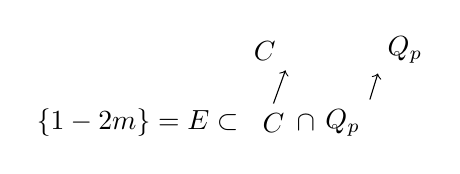
\begin{tikzpicture}
\node[anchor=east] at (0,0) {$\{1-2m\}=E\subset$};
\node (first) at (.32,0) {$\mathbb C$};
\node at (.73,0) {$\cap$};
\node (second) at (1.20,0) {$\mathbb Q_p$};
\node (c) at (.21,.91) {$\mathbb C$};
\node (q) at (1.99,.92) {$\mathbb Q_p$};
\draw[->] (first.north)--(c.south east);
\draw[->] (second.north east)--(q.south west);
\end{tikzpicture}}\endgroup\par}}
\end{GelfandAdjacentEvidence}
\begin{GelfandAdjacentEvidence}{GELFAND-P000502}{12}

и они аналитичны

На самом деле, видимо, правильный аргумент — адельный.
\[
\mathbb Q_p\longrightarrow\mathbb Q_{\ell}\quad(p\ne\ell)\quad
\text{видимо, проще (но неизв.)}
\]
Трудно $\mathbb Q_p\longrightarrow\mathbb Q_p$,

Начал \uuline{Мазур}.

\uline{Меры на \mbox{$p$}-адич. компактных пр-вах.}

$K$ — конечн. расш. $\mathbb Q_p$;\quad
$A$ — целые в $K$;\quad
$A\supset\overline m$ (макс. идеал)

\hfill (корни ур-й с целыми коэфф.)
\[
\operatorname{Card}(A/\overline m)\underset{\mathrm{def}}{=}q.
\]
Комп. анал. мн-зие над $K$.
\[
A^n=\underbrace{A\times\ldots\times A}_{n}
\quad\text{— $n$-мерный шар}
\]
\uline{Анал. мн-зие}: пр-во и пучок ф-й, лок. устр. — шар.

\uline{Теорема} (Серр): $X$ — комп. ан. мн-зие над $K$ разм. $n$. Тогда

а) $X\simeq rA^n$ (аналит. изом.), $r\in\mathbb N$
\Unclear{GELFAND-P000502}{theorem-count}{Число шаров условно набрано как $r$. Возможно $\tau$.}
\end{GelfandAdjacentEvidence}
\begin{GelfandAdjacentEvidence}{GELFAND-P000502}{13}


\SourceFigure{GELFAND-P000502}{serre-disjoint-balls}{Четыре овала и подпись справа.\par\smallskip
{\centering
\begingroup\color{black}\GelfandFitDiagram{\begin{tikzpicture}
\draw (0,0) ellipse (.23 and .18);
\draw (.92,.02) ellipse (.19 and .15);
\draw (1.64,-.03) ellipse (.18 and .13);
\draw (2.38,0) ellipse (.18 and .15);
\node[anchor=west] at (2.84,0) {— непересек. шары};
\end{tikzpicture}}\endgroup\par}}
\end{GelfandAdjacentEvidence}
\begin{GelfandAdjacentEvidence}{GELFAND-P000502}{14}


б) \sout{если}
\[
rA^n\simeq r'A^n\quad
\mathrel{\tikz[baseline=(equiv.base)]\node[draw,ellipse,inner sep=1pt] (equiv) {$\Leftrightarrow$};}
\quad r\equiv r'\ \operatorname{mod}(q-1)
\]
\Unclear{GELFAND-P000502}{serre-cancelled-condition}{Зачёркнутое слово условно прочитано как «если». Знак эквивалентности обведён.}
\end{GelfandAdjacentEvidence}



\Needspace{7\baselineskip}
\begin{GelfandAdjacentEvidence}{GELFAND-P000503}{1}
\SourcePage{GELFAND-P000503}{2}
\[
A=\{a\in K\mid a\text{ целое}\}.\qquad
A=\bigcup_{a_i\ \mathrm{mod}\ m}\{a\equiv a_i\ \mathrm{mod}\ m\}.
\]
\uwave{Как вычислять \mbox{$r$}?}
\Unclear{GELFAND-P000503}{invariant-letter}{Буква условно набрана как $r$.}
\end{GelfandAdjacentEvidence}
\begin{GelfandAdjacentEvidence}{GELFAND-P000503}{2}


\uline{Примеры}: а) $X$ — алг. мн-зие над $A$
(гладкая схема над $\operatorname{Spec}A$).

\sout{Как вычислять \mbox{$r$} из п. а) теор. Серра?}
\Unclear{GELFAND-P000503}{cancelled-question}{Зачёркнутый вопрос прочитан условно. Штрихи особенно густы над обозначением пункта.}
\end{GelfandAdjacentEvidence}
\begin{GelfandAdjacentEvidence}{GELFAND-P000503}{3}


Редукция $X_0\quad
\underset{\text{над }\operatorname{Spec}A.}{\text{(замкн. слой)}}$
— алг. мн-зие на $A/\bar m$
\[
\operatorname{Card}X_0(A/\bar m)=r(X).
\]
\uwave{Пример} схемы: $X=P^1$ или окружность.
\quad 2 афф. прямые скл. $x=y^{-1}$

Редукция: проект. прям. над кон. полем из $q$ элем. — там $q+1$ элем.
\[
q+1=2\ \mathrm{mod}(q-1).
\]
Итак 2 шара:
\SourceFigure{GELFAND-P000503}{two-balls}{У левого контура верх затушёван. Стрелки правого контура направлены к верхнему разрыву. Справа «и» и маленький округлый знак.\par\smallskip
{\centering
\begingroup\color{black}\GelfandFitDiagram{\begin{tikzpicture}
\draw (-.12,.31) arc[start angle=104,end angle=438,x radius=.52,y radius=.31];
\fill (-.06,.29) ellipse (.19 and .09);
\draw[line width=.8pt] (-.39,.20)--(-.17,.36) (.02,.36)--(.21,.19);
\draw[->] (1.50,-.30) arc[start angle=270,end angle=443,x radius=.48,y radius=.31];
\draw[->] (1.50,-.30) arc[start angle=270,end angle=98,x radius=.48,y radius=.31];
\node at (2.31,.00) {и};
\draw[very thick] (2.81,.37) ellipse (.057 and .045);
\end{tikzpicture}}\endgroup\par}}
\end{GelfandAdjacentEvidence}
\begin{GelfandAdjacentEvidence}{GELFAND-P000503}{4}

\[
P^1(K)=\mathbb Q_p\cup\infty,\qquad pA\cup A^{-1}.
\]

б) $X$ — $p$-адич. комп. гр. Ли; она проконечна, у $\forall$ фактора есть порядок.

Порядок: $2^2\,3^\infty\,5^1\,7^0\,11^\infty\ldots$ —
сверхъестеств. число (т. к. делятся друг на друга).
\SourceFigure{GELFAND-P000503}{supernatural-exponent}{Черта слева от показателя принадлежит цифре $5$. Показатель прочитан как $1$.}
\end{GelfandAdjacentEvidence}
\begin{GelfandAdjacentEvidence}{GELFAND-P000503}{5}


Оказывается, $\operatorname{ord}X=p^\infty\cdot N$,
где $(p,N)=1$, $N$ — обычн. целое.
\[
\underline{\underline{N=r(X)}}
\]
$SL_2$ — $(p-1)$ шаров $(=p^2-1\ \mathrm{mod}\ p)$
\SourceFigure{GELFAND-P000503}{sl2-count}{В рукописи написано $p^2-1\ \mathrm{mod}\ p$.}
\end{GelfandAdjacentEvidence}
\begin{GelfandAdjacentEvidence}{GELFAND-P000503}{6}


\SourceFigure{GELFAND-P000503}{margin-fields}{Между $L$ и $K$ стоит густо закрашенный знак. Его форма и направление не установлены.\par\smallskip
{\centering
\begingroup\color{black}\GelfandFitDiagram{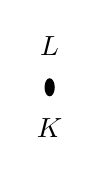
\begin{tikzpicture}
\node at (0,.52) {$L$};
\fill (0,0) ellipse (.065 and .115);
\node at (0,-.52) {$K$};
\end{tikzpicture}}\endgroup\par}}
\end{GelfandAdjacentEvidence}
\begin{GelfandAdjacentEvidence}{GELFAND-P000503}{7}

\uline{Определение}: $L$-мера на $X$ — это $L$-значная конечно-аддит. ф-я на открыто-замкн. подмн-вах $X$.

($X$ — комп. анал. мн-зие).
\Unclear{GELFAND-P000503}{definition-overwrite}{Начало сокращения «анал.» густо переписано.}
\end{GelfandAdjacentEvidence}
\begin{GelfandAdjacentEvidence}{GELFAND-P000503}{8}


\uline{Примеры}: а) $X=\mathbb Z_p$
\SourceFigure{GELFAND-P000503}{clopen-tree}{Из вершины $X$ выходят четыре ветви. В нижних пучках некоторые штрихи сливаются.\par\smallskip
{\centering
\begingroup\color{black}\GelfandFitDiagram{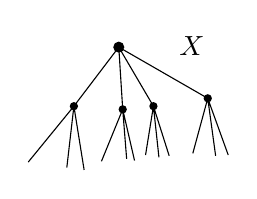
\begin{tikzpicture}
\coordinate (root) at (0,1.65);
\coordinate (a) at (-.57,.90);
\coordinate (b) at (.05,.86);
\coordinate (c) at (.44,.90);
\coordinate (d) at (1.13,1.00);
\draw (root)--(a) (root)--(b) (root)--(c) (root)--(d);
\draw (a)--(-1.15,.19) (a)--(-.66,.12) (a)--(-.44,.09);
\draw (b)--(-.22,.20) (b)--(.10,.23) (b)--(.20,.21);
\draw (c)--(.34,.28) (c)--(.51,.25) (c)--(.64,.27);
\draw (d)--(.94,.30) (d)--(1.23,.27) (d)--(1.39,.28);
\fill (root) circle (2pt);
\foreach \vertex in {a,b,c,d}{\fill (\vertex) circle (1.5pt);}
\node at (.93,1.66) {$X$};
\end{tikzpicture}}\endgroup\par}}
\end{GelfandAdjacentEvidence}
\begin{GelfandAdjacentEvidence}{GELFAND-P000503}{9}


Вершины — откр.-замкн. подмн-ва.

Последовательно строим эти меры. Получ. фунд. сист. окрестностей.
\[
\begin{gathered}
\text{Мера на }X\leftrightarrow
\{\mu(a+(p^m))\in L;\quad a\ \mathrm{mod}(p^m),\ m\in\mathbb N\}.\\
\mu(a+(p^m))=\sum_{b\equiv a\ \mathrm{mod}\ p^m}\mu(b+(p^{m+1}))\}
\end{gathered}
\]
\SourceFigure{GELFAND-P000503}{measure-braces}{На конце каждой из двух строк стоит закрывающая фигурная скобка.}
\end{GelfandAdjacentEvidence}
\begin{GelfandAdjacentEvidence}{GELFAND-P000503}{10}


И это применимо к любому компактному подмн-зию.

\[
\text{б) }\mu(a+(p^m))=\underbrace{\mathrm{const}\cdot p^{-m}}_{\in L}
\quad\text{— \uuline{инвар. меры.}}
\]
На $L$ есть метрика ($p$-ад. модуль).
\[
|\mathrm{const}\cdot p^{-m}|_L\longrightarrow\infty\quad
\text{при }m\longrightarrow\infty.
\]
Чем меньше мн-ва, тем больше мера!!

К нулю не может стремиться! Тогда из неархим. следовало бы, что мера всего равна $0$.

Инвар. меры — плохие.

Самая слабо раст. — ограниченная.
\[
\text{в) }\mu(a+(p^m))=1\text{ при }a<\frac{p^m}{2},\qquad
-1\text{ при }a>p^m/2
\]
\SourceFigure{GELFAND-P000503}{measure-signs}{Слева написано $1$, справа $-1$. В первом пороге дробь вертикальная, во втором записана через косую черту.}
\end{GelfandAdjacentEvidence}
\begin{GelfandAdjacentEvidence}{GELFAND-P000503}{11}

\begin{flushright}
$\Vert$ нетрив. огранич. мера
\end{flushright}
$0<a<p^m$,\quad $(a,p)=1$ \quad Мера на $\mathbb Z_p^*$.
\Incomplete{GELFAND-P000503}{bottom-cancelled-glyph}{Между $0<a<p^m$ и $(a,p)=1$ зачёркнута короткая запись. Чтение не установлено.}
\end{GelfandAdjacentEvidence}



\Needspace{7\baselineskip}
\begin{GelfandAdjacentEvidence}{GELFAND-P000504}{1}
\SourcePage{GELFAND-P000504}{unlabelled}
\uline{Упражнение}: пров. аддитивность. Происх. интерференция.

Интегр. по ней — $\zeta$-ф-и Леопольда — Куботы.

эту меру придумал Мазур.

\uline{Интегралы.}\qquad
$X$, $\mu$ — мера со знач. в $L$.
\SourceFigure{GELFAND-P000504}{field-map-L-to-K}{На правом поле стрелка направлена вниз от $L$ к $K$.\par\smallskip
{\centering
\begingroup\color{black}\GelfandFitDiagram{\begin{tikzpicture}
\node (L) at (0,.86) {$L$};
\node (K) at (0,0) {$K$.};
\draw[->] (L)--(K);
\end{tikzpicture}}\endgroup\par}}
\end{GelfandAdjacentEvidence}
\begin{GelfandAdjacentEvidence}{GELFAND-P000504}{2}


$X\overset f\longrightarrow L$, аналит. ф-я.
\[
\int_X f\,d\mu
\]
\[
R=\{(U_i),\quad\underset{\text{откр.-замкн.}}{U_i}
\text{ — разбиение }X,\quad a_i\in U_i\}
\]
\[
S(f,R)=\sum f(a_i)\mu(U_i).
\]
\[
\int_X f\,d\mu=\lim_R S(f;R)
\]
если предел сущ. при измельчении

\uline{Пример.}\qquad $X=\mathbb Z_p$, $\mu$ — инвар.
\(\bigl(\mu(a+(p^m))=p^{-m}.\bigr)\),

$L=\mathbb Q_p$.\qquad $f=1$ интегрируется

\uuline{\mbox{$f=x$}} — прост. непост.
\[
\int f\,d\mu\quad\text{не сущ.!}
\]
\[
R=\{0\le a\le p^m-1,\quad a\in U_a\equiv\{b\mid b\equiv a\ \mathrm{mod}\ p^m\}.
\]
\Unclear{GELFAND-P000504}{partition-exponent-cancelled}{После $m$ в показателе зачёркнута запись, похожая на $-1$. Следующий знак $-1$ относится к самой границе.}
\end{GelfandAdjacentEvidence}
\begin{GelfandAdjacentEvidence}{GELFAND-P000504}{3}

\[
S(f,R)=\frac1{p^m}\underbrace{\sum_{a=0}^{p^m-1}a}_{\displaystyle\frac{(p^m-1)p^m}{2}}
\longrightarrow-\frac12
\]
\Unclear{GELFAND-P000504}{sum-exponent-cancelled}{У первого $p$ под скобкой после показателя $m$ зачёркнута запись, похожая на $-1$.}
\end{GelfandAdjacentEvidence}
\begin{GelfandAdjacentEvidence}{GELFAND-P000504}{4}


Но это не единств. пред. точка.
\[
R'=\{p^m\in U_0\quad\text{остальное как в }R\}
\]
\uline{Предел будет другой}: измен. ф-и на интервале $\approx$ мере интерв.

\uline{отсюда усл. на меру}: при измельчении отнош. меры к инвар. мере должно $\longrightarrow0$ (это в случае $n=1$).

\uline{Теорема}: пусть $X$ одномерно над $\mathbb Q_p$

1) $\mu$ — мера на $X$ со знач. в $L$, умеренно растущая,
т. е.
\[
U\longrightarrow\underset{\text{точка}}{\bullet}
\Longrightarrow
\left|\frac{\mu(U)}{\mu_{\mathrm{inv}}(U)}\right|_L\longrightarrow0
\]
\Unclear{GELFAND-P000504}{moderate-overwrite}{Начало слова «умеренно» густо наведено.}
\end{GelfandAdjacentEvidence}

($\mu_{\mathrm{inv}}$ — обыч. инв. мер на $\mathbb Z_p$).

2) $f:X\longrightarrow L$ уд. усл. Липшица с показ. $1$

Тогда $\int f\,d\mu$ существует.

\begin{flushright}
$\Vert$ \uwave{След. раз}: конкр. меры и модул. формы.
\end{flushright}


\Needspace{7\baselineskip}
\begin{GelfandAdjacentEvidence}{GELFAND-P000505}{1}
\SourcePage{GELFAND-P000505}{unlabelled}
\Unclear{GELFAND-P000505}{top-right-label}{Надпись за правой рамкой обрезана краем кадра. Чтение не установлено.}
\end{GelfandAdjacentEvidence}
\begin{GelfandAdjacentEvidence}{GELFAND-P000505}{2}


\uwave{10.9.73.}\qquad\uuline{Сем. Гельфанда.}

\uuline{Манин}\quad(\uwave{продолжение}).

$X$ — 1-мерное $p$-адич. пр-во;

$\mu$ — $K$-мера на $X$\qquad
($K$ — конечн. расш. $\mathbb Q_p$)

\underline{$f:X\longrightarrow K$}

\[
R:\quad\text{данные Римана: }\{X=\bigcup_{i=1}^n U_i\,
\text{\sout{\}}},\quad a_i\in U_i\}.
\]
\Unclear{GELFAND-P000505}{riemann-cancelled-brace}{После $U_i$ видна зачёркнутая закрывающая скобка.}
\end{GelfandAdjacentEvidence}
\begin{GelfandAdjacentEvidence}{GELFAND-P000505}{3}

\[
S(f,R)=\sum\mu(U_i)f(a_i).
\]

\uline{Теорема}:

$\exists\int_X f\,d\mu$, если

а) $f$ липшицева с пок. $1$

б) $(U\mapsto\text{точка})\Longrightarrow
\left|\mu(U)/\mu_{\mathrm{inv}}(U)\right|\longrightarrow0$.

\uuline{Пример.}\qquad $X=\mathbb Z_p$;
\[
\mu(a+(p^m))=
\begin{cases}
-1&\text{при }0\le a<\dfrac{p^m}{2}\\
+1&\text{при }\dfrac{p^m}{2}<a<p^m.
\end{cases}
\]
\uwave{Дерево откр.-замкн. подмн-в}:
\SourceFigure{GELFAND-P000505}{clopen-moment-tree}{От верхнего кружка идут три штриха вверх. Внизу две трёхлучевые развилки. У верхней ветви стоит 1.\par\smallskip
{\centering
\begingroup\color{black}\GelfandFitDiagram{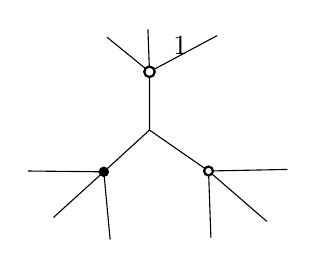
\begin{tikzpicture}
\coordinate (top) at (0,1.66);
\coordinate (fork) at (0,.92);
\coordinate (left) at (-.58,.39);
\coordinate (right) at (.75,.40);
\draw (top)--(-.54,2.10) (top)--(-.02,2.20) (top)--(.86,2.12);
\draw (top)--(fork) (fork)--(left) (fork)--(right);
\draw (left)--(-1.54,.40) (left)--(-1.22,-.19) (left)--(-.50,-.47);
\draw (right)--(1.75,.42) (right)--(1.49,-.24) (right)--(.78,-.45);
\filldraw[fill=white,thick] (top) circle (1.9pt) (right) circle (1.6pt);
\fill (left) circle (1.9pt);
\node at (.39,1.99) {$1$};
\end{tikzpicture}}\endgroup\par}}
\end{GelfandAdjacentEvidence}
\begin{GelfandAdjacentEvidence}{GELFAND-P000505}{4}


$f(x)=x^{2r-1}$\qquad (для $f(x)=x^{2r}$ получится 0).
\Unclear{GELFAND-P000505}{moment-index}{Похожая на $\tau$ буква условно набрана как $r$.}
\end{GelfandAdjacentEvidence}
\begin{GelfandAdjacentEvidence}{GELFAND-P000505}{5}


\[
\int_{\mathbb Z_p}x^{2r-1}\,d\mu=(-1)^r(1-2^{-r})\frac{B_{r-1}}{2r}
\]
\[
\mathbb Z_p=\bigcup_{0\le a<p^{m-1}}\{a+p^m\mathbb Z_p\}.
\]
\SourceFigure{GELFAND-P000505}{union-upper-bound}{В верхней границе $-1$ находится на уровне показателя $m$.}
\end{GelfandAdjacentEvidence}
\begin{GelfandAdjacentEvidence}{GELFAND-P000505}{6}


$R$
\Unclear{GELFAND-P000505}{margin-r}{На левом поле знак густо наведён. Условно прочитан как $R$.}
\end{GelfandAdjacentEvidence}
\begin{GelfandAdjacentEvidence}{GELFAND-P000505}{7}

\[
S(f,R)=-\sum_{0\le a<p^m/2}a^{2r-1}
+\sum_{p^m>a>p^m/2}a^{2r-1}
\]

Есть формулы Вороного, интерпретируемые как вычисление таких интегралов.

\[
\int_{\mathbb Z_p^*}=\int_{\mathbb Z_p}-\int_{p\mathbb Z_p}
\]
\[
\begin{aligned}
\int_{\mathbb Z_p^*}x^{2r-1}\,d\mu
&=(1-p^{2m-1})\int_{\mathbb Z^p}\\
&=(-1)^r(1-p^{2m-1})\cdot(1-2^{-r})\frac{B_{r-1}}{2r}=
\end{aligned}
\]
\SourceFigure{GELFAND-P000505}{lower-powers}{В обоих множителях показатель написан как $2m-1$.}
\end{GelfandAdjacentEvidence}
\begin{GelfandAdjacentEvidence}{GELFAND-P000505}{8}

\SourceFigure{GELFAND-P000505}{lower-integral-domain}{У $\mathbb Z$ буква $p$ написана вверху справа.}
\end{GelfandAdjacentEvidence}


(вычислено преобр. Меллина характеров)
\[
=(\ldots)\zeta_{(p)}(1-2r)
\]


\Needspace{7\baselineskip}
\begin{GelfandAdjacentEvidence}{GELFAND-P000506}{1}
\SourcePage{GELFAND-P000506}{5}
Рассм. $X=\operatorname{Hom}(\mathbb Z_p^*;K^*)$.
\Unclear{GELFAND-P000506}{hom-codomain}{Знак вверху у $K$ слит со скобкой. Условно прочитан как звёздочка.}
\end{GelfandAdjacentEvidence}
\begin{GelfandAdjacentEvidence}{GELFAND-P000506}{2}

\[
\mathbb Z_p^*=(\mathbb Z/p\mathbb Z)^*\times(1+p)^{\mathbb Z_p}.
\]
$\chi\in X\Longrightarrow\chi=\chi_0\cdot\chi_1$, где
\[
\begingroup\color{black}\GelfandFitDiagram{\begin{tikzpicture}[baseline=(conditions.base)]
\node[inner sep=2pt] (conditions) {$\begin{aligned}
\chi_0&=1\quad\text{на }(1+p)^{\mathbb Z_p}.\\
\chi_1&=1\quad\text{на }(\mathbb Z/p\mathbb Z)^*.
\end{aligned}$};
\draw ([xshift=-2pt,yshift=7pt]conditions.south west)
  |- ([xshift=4pt]conditions.south east);
\end{tikzpicture}}\endgroup
\]
\[
\forall u\in\mathbb Z_p^*: \quad u=\varepsilon\cdot(1+p)^a,\qquad
\text{где }\varepsilon^{p-1}=1,\quad a\in\mathbb Z_p
\]

Поэтому
\SourceFigure{GELFAND-P000506}{character-product}{%
\begingroup\color{black}\GelfandFitDiagram{\begin{tikzpicture}
\node[inner sep=1pt] at (0,0) {$X=$};
\node[inner sep=1pt] (finite) at (.8,0) {$X_0$};
\node[inner sep=1pt] at (1.4,0) {$\times$};
\node[inner sep=1pt] (adic) at (2,0) {$X_1$};
\draw (finite.south) -- ++(0,-.25);
\draw (adic.south east) -- ++(.20,-.25);
\node[anchor=north] at (.8,-.49) {конечн.};
\node[anchor=north west,inner sep=1pt] at (2.35,-.49) {$p$-адич. мн-зие.};
\end{tikzpicture}}\endgroup}
\end{GelfandAdjacentEvidence}
\begin{GelfandAdjacentEvidence}{GELFAND-P000506}{3}


\hfill Итак: $X$ — $p$-адич. мн-зие\par

\[
\chi_1(1+p)=1+t,\qquad t\in\overline{m}.\qquad
\text{(обозначение: }\chi_{(t)}\text{)}
\]
Отсюда $X_1\cong\overline{m}$ (но другой закон композиции)
\SourceFigure{GELFAND-P000506}{composition-retrace}{В слове «но» первая буква густо наведена.}
\end{GelfandAdjacentEvidence}
\begin{GelfandAdjacentEvidence}{GELFAND-P000506}{4}


\uline{Теорема}. Если $\mu$ умеренно растёт (медл., чем инвар.), то
\[
\int_{\mathbb Z_p^*}\chi\,d\mu\quad\text{аналитична по $\chi$}.
\]

\uline{Подробнее}:
\[
\int\chi_{(t)}\,d\mu=F(t)\in K[[t]]
\]
сходится при $|t|<1$.

Далее: $\int x^s\,d\mu$ аналитичен по $s$ при $s\equiv0\ (\operatorname{mod}(p-1))$
и при $s=k\operatorname{mod}(p-1)$
\SourceFigure{GELFAND-P000506}{power-integrand}{Подынтегральное выражение читается как $x^s$.}
\end{GelfandAdjacentEvidence}
\begin{GelfandAdjacentEvidence}{GELFAND-P000506}{5}


\begin{center}— · —\end{center}
\uline{Модулярные формы}. $\Gamma=SL(2,\mathbb Z)/(\pm1)$ действует на
\[
H=\{z\in\mathbb C\mid\operatorname{Im}z>0\},\qquad w\equiv0\ (2),\qquad w\geq0
\]
$\underline{P}_w$: \uwave{Параб. формы веса \mbox{$w+2$} на \mbox{$H$}:}

а) $\varphi(z)(dz)^{\frac{w+2}{2}}$ $\Gamma$-инвариантен

б) $\varphi(z)=\displaystyle\sum_{n=1}^\infty a_ne^{2\pi inz}$

1-я нетрив. ф-я при $w+2=12$ с пропусками до $26$
(1 мерные), потом всюду кон-мерное пр-во
[Зачёркнуто: \Incomplete{GELFAND-P000506}{modular-cancellation}{Под густой правкой чтение не установлено.}
\end{GelfandAdjacentEvidence}
]
\[
w+2=12\quad\Longrightarrow\quad
e^{2\pi iz}\prod_{n=1}^\infty(1-e^{2\pi inz})^{24}
=\sum_{n=1}^\infty\tau(n)e^{2\pi inz}
\]
\begin{center}— · —\end{center}
В $P_w$ сущ. базис из форм с целыми алг. коэффициентами


\Needspace{7\baselineskip}
\begin{GelfandAdjacentEvidence}{GELFAND-P000507}{1}
\SourcePage{GELFAND-P000507}{unlabelled}
и такой, что если $\displaystyle\sum_1^\infty a_ne^{2\pi inz}$ — эл. этого базиса, то
\[
\sum a_nn^{-s}=\prod_p\frac{1}{1-a_pp^{-s}+p^{w+1-\text{[?]}}}.
\]
\Unclear{GELFAND-P000507}{euler-exponent}{Конец показателя первого произведения переписан. Чтения: $2s$ или знак, похожий на $k$.}
\end{GelfandAdjacentEvidence}
\begin{GelfandAdjacentEvidence}{GELFAND-P000507}{2}


(По каждой [Зачёркнуто: $p$-адич.; над строкой, в обводке: параб.]
форме построим дальше пар. меру)
\SourceFigure{GELFAND-P000507}{form-insertion}{Вписанное «параб.» отведено обводкой к зачёркнутому слову.}
\end{GelfandAdjacentEvidence}
\begin{GelfandAdjacentEvidence}{GELFAND-P000507}{3}


\uwave{Опер. Гекке}: посм. каковы $a$, если
\[
\sum a_nn^{-s}=
\frac{1}{\left(1-\lambda_pp^{-s}+p^{w+1-2s}\right)}
\left(\sum\ldots\right)
\]
т. е.
\[
\sum a_nn^{-s}=
\underset{\substack{\vert\\\text{изв.}}}{\left(\qquad\right)}
\underset{\substack{\vert\\\text{неопр.}}}
  {\left(\sum b_nn^{-s}\right)}
\]
\SourceFigure{GELFAND-P000507}{factor-labels}{Пустые скобки подписаны «изв.», ряд подписан «неопр.».}
\end{GelfandAdjacentEvidence}
\begin{GelfandAdjacentEvidence}{GELFAND-P000507}{4}

\[
1-\lambda p^{-s}+p^{w+1-2s}=(1-\alpha_1p^{-s})(1-\alpha_2p^{-s}).
\]
Получ. лин. условие на коэфф. $a_n$.

Всё вместе — беск. матрица.
\Unclear{GELFAND-P000507}{matrix-afterword}{Знак после точки густо переписан. Чтение не установлено.}
\end{GelfandAdjacentEvidence}
\begin{GelfandAdjacentEvidence}{GELFAND-P000507}{5}


Это усл. $\Longleftrightarrow$ Вект. коэфф. — соб. для оператора Гекке.

Выпишем его не на коэфф. Фурье, а на ф-ю.
\[
(\Phi\mid T_p)(z)\underset{\mathrm{def}}{=}
p^{w+1}\Phi(pz)+p^{-1}\sum_{k=0}^{p-1}\Phi\left(\frac{z+k}{p}\right).
\]
Соб. ф-и $\Longleftrightarrow$ из соотв. ряда Дирихле выд. $p$-множитель.
\[
(P_w\mid T_p)=P_w.
\]

\uline{Меры: на \mbox{$\mathbb Z_p^*$}, связ. с}
$\varphi$, $\varphi\mid T_p=\lambda_p\varphi\quad\forall p$.

[Зачёркнуто: \Unclear{GELFAND-P000507}{measure-value-cancellation}{Возможно, $\mathbb Q_p$. Чтение под зачёркиванием не установлено.}
\end{GelfandAdjacentEvidence}
\begin{GelfandAdjacentEvidence}{GELFAND-P000507}{6}
]
со знач. $\{\mathbb Q_p(\lambda_1,\ldots,\lambda_p,\ldots)\}_p$

\uwave{Полумеры со знач. в}
[Зачёркнуто: \Unclear{GELFAND-P000507}{field-cancellation}{Возможно, $\mathbb Q$. Чтение под зачёркиванием не установлено.}
\end{GelfandAdjacentEvidence}
\begin{GelfandAdjacentEvidence}{GELFAND-P000507}{7}
]
\uwave{\mbox{$\mathbb C$}.}

$x\in\mathbb Q$.\qquad
$P(x)=\displaystyle\int_x^{i\infty}\Phi(z)\,dz$
\SourceFigure{GELFAND-P000507}{period-path}{%
\begingroup\color{black}\GelfandFitDiagram{\begin{tikzpicture}
\draw (-1.2,0) -- (1.4,0);
\draw[->] (0,1.35) -- (0,0);
\end{tikzpicture}}\endgroup}
\end{GelfandAdjacentEvidence}
\begin{GelfandAdjacentEvidence}{GELFAND-P000507}{8}


Сходимость: на верхн. конце очевидна $(e^{2\pi inz}\to0)$, а на нижнем неясно.
Из функц. ур-я: и на нижн. конце сход., но завис. от $x$ не непр. (из тонкой арифметики).
В иррац. точках как правило расходится. $P(x+1)=P(x)$.

$\lambda_pP(x)=\displaystyle\int_x^{i\infty}\Phi(z)\mid T_p\,dz$
заменяем и получ. функц. ур-е
\[
\lambda_pP(x)=p^wP(px)+\sum_{k=0}^{p-1}P\left(\frac{x+k}{p}\right)
\]
\Unclear{GELFAND-P000507}{isolated-p}{Над аргументом правого слагаемого стоит отдельный знак, похожий на $p$ или $P$.}
\end{GelfandAdjacentEvidence}

\[
\frac{a}{p^m}\sim a+p^m\mathbb Z_p.
\]
Мера $P\left(\frac{a}{p^m}\right)$ даёт почти конечн. аддитивность.


\Needspace{7\baselineskip}
\begin{GelfandAdjacentEvidence}{GELFAND-P000508}{1}
\SourcePage{GELFAND-P000508}{6}
\uline{Поправка}:
\[
\mu_\Phi(a+p^m\mathbb Z_p)=
\varrho^{-m}P\left(\frac{a}{p^m}\right)
-p^w\varrho^{-(m+m)}P\left(\frac{a}{p^{m+1}}\right)\qquad (?).
\]
\SourceFigure{GELFAND-P000508}{correction-formula}{Во втором показателе у $\varrho$ написано $-(m+m)$. В последнем знаменателе написано $p^{m+1}$. Знак $(?)$ стоит в рукописи.}
\end{GelfandAdjacentEvidence}
\begin{GelfandAdjacentEvidence}{GELFAND-P000508}{2}


Получ. мера на $\mathbb Z_p^*$.

\sout{До след. раз}
\SourceFigure{GELFAND-P000508}{closing-cancellation}{Фраза зачёркнута двумя чертами. Последнее слово читается «раз».}
\end{GelfandAdjacentEvidence}


\begin{center}— · —\end{center}


\Needspace{7\baselineskip}
\begin{GelfandAdjacentEvidence}{GELFAND-P000509}{1}
\SourcePage{GELFAND-P000509}{unlabelled}
17.9.73. \quad\uline{Сем. Гельфанда.}
\Unclear{GELFAND-P000509}{date-day}{Вторая цифра дня переписана. Поверх прежних штрихов читается «7».}
\end{GelfandAdjacentEvidence}
\begin{GelfandAdjacentEvidence}{GELFAND-P000509}{2}


\uline{Ю.И. Манин} (продолжение)
\[
P(x)=\int_x^{i\infty}\Phi(z)\,dz
\]
Рассм. ур-е $\varrho^2-\lambda_p\varrho+p^{w+1}=0$.
и $\varrho$ — любой его корень

\uline{Предложение}. Положим
\[
\mu_\Phi\bigl(a+(p^{m+1})\bigr)
=\varrho^{-m}P\left(\frac{a}{p^{m+1}}\right)
-p^w\varrho^{-(m+1)}P\left(\frac{a}{p^m}\right).
\]
Тогда это полумера (на $\mathbb Z_p^*$ со знач. в $\mathbb C$ и кон.-аддитивна).

Рассм. \uwave{периоды формы}:
\[
\tau_k(\varphi)=\int_0^{i\infty}\varphi(z)z^k\,dz,\qquad 0\leq k\leq w.
\]
\[
L_\varphi(s)=\sum_{n=1}^\infty\lambda_n n^{-s}
=\frac{(2\pi)^s}{\Gamma(s)}\int_0^\infty\varphi(iy)y^{s-1}\,dy
\]
\[
\tau_k(\varphi)=\frac{k!\,i^{k+1}}{(2\pi)^{k+1}}L_\varphi(k+1)
\]
$[1,w+1]$ — крит. полоса (отн. неё функц. ур-е)

\uline{Предложение}. $\forall x\in\mathbb Q,\ 
P(x)\in\displaystyle\sum_{k=0}^w\mathbb Z\cdot\tau_k(\Phi)$

$\operatorname{Re}$ и $\operatorname{Im}$ им. общ. трансценд. множитель, поделив на к-рый получим алгебраические
\[
\int_{b/d}^{i\infty}\Phi(z)\,dz=\int_0^{i\infty}-\int_0^{b/d}
\]
(в окр. точек оси интегр. по геодезическим).

\uline{Контур:}
\SourceFigure{GELFAND-P000509}{contour}{%
\begingroup\color{black}\GelfandFitDiagram{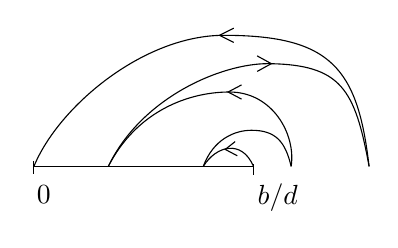
\begin{tikzpicture}[x=.90cm,y=.90cm]
\draw (0,0) -- (3.1,0);
\draw (0,-.10) -- (0,.08);
\draw (3.1,-.12) -- (3.1,.04);
\node[below] at (.14,-.13) {$0$};
\node[below right] at (3.02,-.10) {$b/d$};
\draw (0,0) .. controls (.35,.85) and (1.55,1.85) .. (2.68,1.85)
  .. controls (4.2,1.85) and (4.57,1.38) .. (4.73,0);
\draw (1.05,0) .. controls (1.52,.98) and (2.65,1.45) .. (3.30,1.45)
  .. controls (4.34,1.44) and (4.53,1.09) .. (4.73,0);
\draw (1.05,0) .. controls (1.45,.78) and (2.18,1.05) .. (2.76,1.05)
  .. controls (3.37,1.05) and (3.70,.45) .. (3.63,0);
\draw (2.39,0) .. controls (2.53,.38) and (2.83,.51) .. (3.07,.51)
  .. controls (3.42,.51) and (3.55,.34) .. (3.63,0);
\draw (2.39,0) .. controls (2.57,.29) and (2.93,.39) .. (3.10,0);
\draw (2.82,1.95) -- (2.62,1.85) -- (2.82,1.75);
\draw (3.15,1.56) -- (3.35,1.45) -- (3.15,1.34);
\draw (2.93,1.15) -- (2.74,1.05) -- (2.93,.95);
\draw (2.84,.35) -- (2.70,.24) -- (2.87,.15);
\end{tikzpicture}}\endgroup\par
\smallskip Внутренние дуги частично перекрываются. Направление четвёртой дуги сверху не установлено.}
\end{GelfandAdjacentEvidence}
\begin{GelfandAdjacentEvidence}{GELFAND-P000509}{3}


из разл. в непр. дробь
\[
\frac bd=\frac{b_m}{d_m},\quad\frac{b_{m-1}}{d_{m-1}},\quad
\ldots,\quad\frac{b_0}{d_0}=\frac01
\]
\[
g_k=\begin{pmatrix}
b_k&(-1)^{k-1}b_{k-1}\\
d_k&(-1)^{k-1}d_{k-1}
\end{pmatrix}\in SL(2,\mathbb Z).
\qquad\text{(выб. знаки).}
\]
\[
\begin{aligned}
\int_0^{b/d}\varphi(z)\,dz
&=\sum_{k=0}^m\int_{b_{k-1}/d_{k-1}}^{b_k/d_k}\Phi(z)\,dz\\
&=\sum_{k=1}^m\int_{g_k(0)}^{g_k(i\infty)}\varphi(z)\,dz\\
&=\sum_{k=1}^m\int_0^{i\infty}\varphi(z)
  \bigl(d_kz+(-1)^{k-1}d_{k-1}\bigr)^w\,dz.
\end{aligned}
\]
\SourceFigure{GELFAND-P000509}{decomposition-lower-index}{В первой сумме написано $k=0$. В следующих двух написано $k=1$.}
\end{GelfandAdjacentEvidence}
\begin{GelfandAdjacentEvidence}{GELFAND-P000509}{4}

Это целочисл. лин. комб. $\tau_k(\varphi)$.

Резюме:
\[
P\left(\frac bd\right)=\sum F(d_k,d_{k-1})
\]
$F$ — многочлен (форма) степ. $w$

Отсюда арифметический хар.
\[
P\left(\frac bd\right)=\sum_{k=0}^w A_k\left(\frac bd\right)\tau_k(\varphi)
\]
\hfill — выделение иррациональностей\par

При этом выраж. аддит. не очевидна...
\SourceFigure{GELFAND-P000509}{bottom-abbreviation}{Сокращение перед «аддит.» читается «выраж.».}
\end{GelfandAdjacentEvidence}


\[
\begin{aligned}
k\text{ — чётно}&\quad\Rightarrow\quad\tau_k(\varphi)\ \text{чисто мнимые}\\
k\text{ — нечётно}&\quad\Rightarrow\quad\tau_k(\varphi)\ \text{вещественно}
\end{aligned}
\]


\Needspace{7\baselineskip}
\begin{GelfandAdjacentEvidence}{GELFAND-P000510}{1}
\SourcePage{GELFAND-P000510}{unlabelled}
\Unclear{GELFAND-P000510}{upper-right-label}{Знак в правом верхнем углу имеет две стойки и соединительный штрих. Возможны «II» и «И».}
\end{GelfandAdjacentEvidence}
\begin{GelfandAdjacentEvidence}{GELFAND-P000510}{2}


\uuline{Предложение}.
\[
\exists\ \omega^+,\omega^-\in\mathbb C,\qquad
\left(\frac{\tau_0}{\omega^+},\frac{\tau_2}{\omega^+},\ldots,\frac{\tau_w}{\omega^+}\right),
\quad\left(\frac{\tau_1}{\omega^-},\ldots,\frac{\tau_{w-1}}{\omega^-}\right)\quad-
\]
— алгебраические (из поля, в к-ром лежат коэффициенты $\Phi$)

\uline{Док-во}.

\uline{Линейные ур-я для \mbox{$\tau_k(\Phi)$}.}

а) \uline{Эйхлер} — \uline{Шимура}; зависят лишь от $w$:
\[
SL(2,\mathbb Z)/(\pm1).\qquad
\text{Рассм. }\ s=\begin{pmatrix}0&1\\-1&0\end{pmatrix},
\quad t=\begin{pmatrix}1&-1\\1&0\end{pmatrix}
\quad\text{(образующие).}
\]
\SourceFigure{GELFAND-P000510}{generator-diagrams}{%
\begingroup\color{black}\GelfandFitDiagram{\begin{tikzpicture}
\node at (-.55,0.57) {$s$};
\draw[->] (0,0) -- (0,1);
\draw[->] (.37,1.05) -- (.37,.12);
\node[anchor=west] at (.62,.55) {мен. ориент.};
\node at (-.55,-.92) {$t$};
\draw[->] (0,-1.40) -- (.06,-.36);
\draw[->] (.87,-1.18) -- (.94,-.30);
\draw[->] (.88,-.97) .. controls (.58,-.69) and (.29,-.84) .. (.09,-1.06);
\end{tikzpicture}}\endgroup}
\end{GelfandAdjacentEvidence}
\begin{GelfandAdjacentEvidence}{GELFAND-P000510}{3}

\[
\left(\int_0^{i\infty}+\int_{s(0)}^{s(i\infty)}\right)\Phi(z)\,dz
=0=\left(\int_0^{i\infty}+\int_{t(0)}^{\ldots}+\ldots\right)
\]
\[
\underline{\tau_k(\Phi)+(-1)^k\tau_{w-k}(\varphi)=0}
\qquad\text{(и следств. функц. ур-я)}
\]
\[
\int_0^{i\infty}\varphi(z)
\left[z^k+z^{w-k}(z-1)^k+(-1)^k(z-1)^{w-k}\right]\,dz=0.
\]
Это и даёт иск. лин. ур-е отн. $\tau_k$.
\[
S_{w+2}=\text{$R$-пр-во форм $\varphi$ с вещ. коэфф.}
\]
\[
S_{w+2}\longrightarrow R
\]
\SourceFigure{GELFAND-P000510}{period-parity-map}{%
\begingroup\color{black}\GelfandFitDiagram{\begin{tikzpicture}
\node (form) at (0,0) {$\varphi$};
\node[anchor=west] (even) at (.76,.52) {$\dfrac1i(\tau_0(\Phi),\tau_2(\varphi),\ldots)$};
\node[anchor=west] (odd) at (.76,-.59) {$(\tau_1(\varphi),\ldots,\tau_{w-1}(\varphi))$};
\draw[->] (form.east) -- (even.west);
\draw[->] (form.east) -- (odd.west);
\end{tikzpicture}}\endgroup}
\end{GelfandAdjacentEvidence}
\begin{GelfandAdjacentEvidence}{GELFAND-P000510}{4}


В пр-вах периодов выд. подпр-ва, зад. ур-ями.
\SourceFigure{GELFAND-P000510}{solution-space-map}{%
\(\displaystyle
S_{w+2}
\left.\begin{array}{cc}\nearrow&S^+\\\searrow&S^-\end{array}\right\}
\underset{\mathrm{def}}{=}
\)\par\smallskip
пр-ва решений ур-й Sh.-Eich.}
\end{GelfandAdjacentEvidence}
\begin{GelfandAdjacentEvidence}{GELFAND-P000510}{5}


\uuline{Теорема}.
\[
\begin{aligned}
\text{а)}\quad&S_{w+2}\overset{\sim}{\longrightarrow}S^-\\
\text{б)}\quad&S_{w+2}\hookrightarrow S^+\qquad
\text{влож.}\quad\operatorname{codim}1.
\end{aligned}
\]

\uuline{Теорема}.
\SourceFigure{GELFAND-P000510}{hecke-period-map}{%
\begingroup\color{black}\GelfandFitDiagram{\begin{tikzpicture}
\node (source) at (0,0) {$S_{w+2}$};
\node (target) at (1.95,0) {$S^-$};
\draw[->] (source.east) -- node[above] {$\sim$} (target.west);
\node at (0,-.66) {$T_p$};
\node[draw,ellipse,inner sep=2pt] at (1.95,-.66) {$T_p^-$};
\node[anchor=west] at (2.65,-.66) {(оп. Гекке).};
\node[anchor=north] at (1.95,-.98) {матрица из $\mathbb Z[\lambda_p]$};
\end{tikzpicture}}\endgroup}
\end{GelfandAdjacentEvidence}
\begin{GelfandAdjacentEvidence}{GELFAND-P000510}{6}


Здесь
\[
(\Phi\mid T_p)(z)=p^{w+1}\varphi(pz)
-p^{-1}\sum_{k=0}^{p-1}\varphi\left(\frac{z+k}{p}\right)
\]
\SourceFigure{GELFAND-P000510}{hecke-minus}{Перед $p^{-1}\sum$ написан знак минус.}
\end{GelfandAdjacentEvidence}
\begin{GelfandAdjacentEvidence}{GELFAND-P000510}{7}

Соб. ф-и опер. Гекке $\Leftrightarrow$
[Зачёркнуто: \Incomplete{GELFAND-P000510}{hecke-cancellation}{Чтение под густой правкой не установлено.}
\end{GelfandAdjacentEvidence}
]
разлаг. в Эйл. произвед.

$T_p^-$ — запись в терм. периодов (лин. форма однозн. опред.)

\uline{Приложение}.
\[
\begin{aligned}
w&=10,\qquad S_{12}=R\cdot e^{2\pi iz}
 \prod_{n=1}^\infty(1-e^{2\pi inz})^{24}\\
 &=R\left(\sum_{n=1}^\infty\tau(n)e^{2\pi inz}\right)
\end{aligned}
\]
\hfill (ф-я Рамануджана)\par

\uwave{Тожд. Рамануджана}
\[
\tau(n)\equiv\sum_{d\mid n}d^{11}\pmod{691}
\]


\Needspace{7\baselineskip}
\begin{GelfandAdjacentEvidence}{GELFAND-P000511}{1}
\SourcePage{GELFAND-P000511}{unlabelled}
\uuline{Меры}.
\[
\begin{aligned}
P^+(x)&=\frac{i}{\omega^+}\operatorname{Im}\int_x^{i\infty}\varphi(z)\,dz,\\
P^-(x)&=\frac{1}{\omega^-}\operatorname{Re}\int_x^{i\infty}\Phi(z)\,dz
\end{aligned}
\]
\[
\mu_\varphi^\pm\bigl(a+(p^{m+1})\bigr)
\underset{\mathrm{def}}{=}
\varrho^{-m}P^\pm\left(\frac{a}{p^{m+1}}\right)
-p^w\varrho^{-(m+1)}P^\pm\left(\frac{a}{p^m}\right)
\]
\Unclear{GELFAND-P000511}{measure-overwriting}{В последнем члене $P$ и показатель при $p$ переписаны. Условно прочитано $P^\pm(a/p^m)$.}
\end{GelfandAdjacentEvidence}
\begin{GelfandAdjacentEvidence}{GELFAND-P000511}{2}

меры с алг. знач. и можно пополнять.
\Unclear{GELFAND-P000511}{measure-note}{Последний глагол условно прочитан «пополнять». Возможно «пополнить».}
\end{GelfandAdjacentEvidence}
\begin{GelfandAdjacentEvidence}{GELFAND-P000511}{3}


\uwave{Рост}. $P^\pm$ им. огранич. знаменатели.
Они могут вылезти из-за $\varrho$.
\[
\varrho^2-\lambda_p\varrho+p^{w+1}=0
\]
\[
\begin{cases}
\varrho_1\cdot\varrho_2=p^{w+1}\\
\varrho_1+\varrho_2=\lambda_p.
\end{cases}
\]
Тип. случай: \uwave{\mbox{$\lambda_p$} вз. пр. с \mbox{$p$}}
$\Rightarrow$ один корень даёт огр. меру, другой растущую!

Неизв. связь [зачёркнуто:
\Incomplete{GELFAND-P000511}{cancelled-middle}{Чтение между «связь» и следующим символом не установлено.}
\end{GelfandAdjacentEvidence}
\begin{GelfandAdjacentEvidence}{GELFAND-P000511}{4}
]
$\lambda_p$ и $p$.

\uline{Интегралы} (пр. Меллина от $p$-ад. хар.)
\[
\ldots\int_{\mathbb Z_p^*}\chi\,d\mu_\Phi^\pm
\]
Манин умеет лишь для хар. конечного пор. $\chi:\mathbb Z_p^*\to K^*$,
$\chi^m=1$ и примитивный.

\uline{Теорема}
\[
\ldots\int_{\mathbb Z_p^*}\chi\,d\mu_\varphi^\pm=\ldots L_\varphi(1,\chi),
\]
где
\[
L_\Phi(s,\chi)=\sum_{n=1}^\infty\chi(n)a_n n^{-s}
\]
\[
\ldots\dot L_\varphi(1,\chi)
=\ldots\int_{R_+^*}\varphi_\chi(z)\,dz,
\qquad\text{где }\Phi_\chi=\sum\chi(n)a_ne^{2\pi inz}.
\]
\Unclear{GELFAND-P000511}{l-dot}{Отдельная точка над $L$ видна в рукописи. Её значение не установлено.}
\end{GelfandAdjacentEvidence}
\begin{GelfandAdjacentEvidence}{GELFAND-P000511}{5}


\uline{О гипотезах Лихтенбаума}: \uwave{о связи \mbox{$K$}-групп, алг. полей с
\mbox{$\zeta$}-ф-ми в цел. точках.}
\[
\sum_{n=1}^\infty\frac{1}{n^2}=\frac{\pi^2}{6},\qquad
\underset{\text{Впервые есть гипотеза}}{%
\sum_{n=1}^\infty\frac{1}{n^3}=2\pi^2\lvert K_4\mathbb Z\rvert\cdot e_5(\alpha_5)}
\]
$\alpha_5$ — образующая $K_5\mathbb Z$. (своб. части)

$e_5$ — гомом. в вещ. числа (нек-рый)

Не док., что $\displaystyle\sum_1^\infty\frac{1}{n^3}$ трансценд.
Пост. Эйлера тоже не док.

\Incomplete{GELFAND-P000511}{cancelled-bottom}{Текст внутри прямоугольника густо зачёркнут. Чтение не установлено.}
\end{GelfandAdjacentEvidence}



\Needspace{7\baselineskip}
\begin{GelfandAdjacentEvidence}{GELFAND-P000512}{1}
\SourcePage{GELFAND-P000512}{unlabelled}
\Unclear{GELFAND-P000512}{upper-right-edge}{У правого верхнего края видны обрезанные штрихи. Чтение не установлено.}
\end{GelfandAdjacentEvidence}
\begin{GelfandAdjacentEvidence}{GELFAND-P000512}{2}


\uuline{24.9.73.}\qquad\uuline{Сем. Гельфанда.}

\uwave{Пинкус;}\quad
\uline{Дуглас, Кобурн, Вилнейер и Зингер;}\quad
\uwave{Хелтон и Роджер Хау. (Howe)}
\Unclear{GELFAND-P000512}{upper-names}{Фамилия после «Кобурн» условно прочитана «Вилнейер». Средние буквы слиты.}
\end{GelfandAdjacentEvidence}
\begin{GelfandAdjacentEvidence}{GELFAND-P000512}{3}


(интересные работы по функц. анализу).

\uline{Теорема} (\uwave{Helton, How}). близко к раб. Крейна, Гохберга, Симоненко и т. д.

Пусть $B$ — билин. форма от 2-х многочленов
[вставлено над строкой: от 2 перем.], причем
\[
B(P_1(Q),P_2(Q))=0,
\]
если $P_1(z),P_2(z)$ — полин. от 1-го пер. $z$,
а $Q$ — полин. от любого числа перем. Тогда
\[
B(R,S)=L(\{R,S\}),\qquad \{R,S\}\ \text{— скобка Пуассона}
\]
\uwave{\mbox{$L$} — лин. форма.}
\SourceFigure{GELFAND-P000512}{two-variable-insertion}{Вставка «от 2 перем.» обведена и отведена к месту после слова «многочленов».}
\end{GelfandAdjacentEvidence}
\begin{GelfandAdjacentEvidence}{GELFAND-P000512}{4}


\begin{center}— · —\end{center}
Пусть $U,V$ — самосопр. и такие, что они коммутируют mod ядерных.
Тогда
\[
\operatorname{Tr}\{[R(U,V),S(U,V)]\}=\iint\{R,S\}\,d\sigma
\]
$R,S$ — многочлены, порядок в них $U$ и $V$ безразличен.

\begin{center}— · —\end{center}
\uline{Кн.}\quad\uuline{Douglas'а}\quad\uwave{Banach algebras technique.}

$\Rightarrow$ в $p$-адич. случае вместо дифф. операторов нужны прав. подобранные норм. кольца.

\begin{center}— · —\end{center}
\uline{Кириллов.}

\uline{L. Brown, R. Douglas, P. Fillmore.}

\uline{Расширения бан. алгебр (нетрадиц. типа).}

$\mathcal K$ — алг. комп. операторов в сеп. гильб. пр-ве.

\uline{Опр. 1.}
\[
0\to\mathcal K\to\mathcal A\to C(X)\to0,\qquad X\ \text{— компакт}
\]
Расш. обр. группу $\operatorname{Ext}(X)=\operatorname{Ext}_1(X)$.

\uline{Другое определение даёт ту же группу:}

\uline{Опр. 2.}
\SourceFigure{GELFAND-P000512}{embedding-bracket}{%
\begingroup\color{black}\GelfandFitDiagram{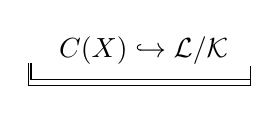
\begin{tikzpicture}
\node[inner xsep=8pt] (embedding) {$C(X)\hookrightarrow\mathcal L/\mathcal K$};
\draw ([xshift=-2pt,yshift=4pt]embedding.south west) |-
 ([yshift=-2pt]embedding.south east) -- ++(0,5pt);
\draw ([xshift=-3pt,yshift=4pt]embedding.south west) |-
 ([yshift=-4pt]embedding.south east) -- ++(0,7pt);
\end{tikzpicture}}\endgroup}
\end{GelfandAdjacentEvidence}
\begin{GelfandAdjacentEvidence}{GELFAND-P000512}{5}


1) рассм. все влож.

2) вложе., отлич. на унит. опер., отождествл. (ун. экв. $UAU^{-1}$).

3) Вложе. вида $C(X)\to\mathcal L\to\mathcal L/\mathcal K$ счит. трив.

Классы эквив. тогда обр. группу.
\SourceFigure{GELFAND-P000512}{parallel-embeddings}{%
\begingroup\color{black}\GelfandFitDiagram{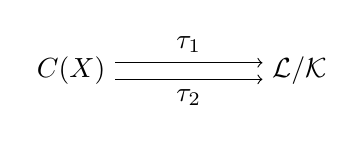
\begin{tikzpicture}
\node (functions) at (0,0) {$C(X)$};
\node (quotient) at (2.9,0) {$\mathcal L/\mathcal K$};
\draw[->] ([yshift=3pt]functions.east) -- node[above] {$\tau_1$} ([yshift=3pt]quotient.west);
\draw[->] ([yshift=-3pt]functions.east) -- node[below] {$\tau_2$} ([yshift=-3pt]quotient.west);
\end{tikzpicture}}\endgroup}
\end{GelfandAdjacentEvidence}
\begin{GelfandAdjacentEvidence}{GELFAND-P000512}{6}

$\tau_1\oplus\tau_2$ уже в $H_1\oplus H_2\cong H$

Функтор
\SourceFigure{GELFAND-P000512}{functor-arrow}{%
\begingroup\color{black}\GelfandFitDiagram{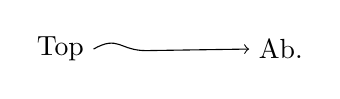
\begin{tikzpicture}
\node (top) at (0,0) {\uwave{Top}};
\node (ab) at (2.8,0) {\uwave{Ab.}};
\draw[->] (top.east) .. controls (.74,.18) and (.75,-.02) .. (1.09,-.02) -- (ab.west);
\end{tikzpicture}}\endgroup}
\end{GelfandAdjacentEvidence}
\begin{GelfandAdjacentEvidence}{GELFAND-P000512}{7}


\uline{Осн. результат:} функтор $\operatorname{Ell}(X)$ сводится к
$\operatorname{Ext}(X)$ (отв. на вопрос Атьи).
\[
\operatorname{Ext}_{1-n}(X)=
\operatorname{Ext}\left(
\underset{\substack{\vert\\\text{\mbox{$n$}-кр. надстройка}}}{S^nX}
\right)
\]
\SourceFigure{GELFAND-P000512}{suspension-pointer}{Под $S^nX$ виден короткий штрих к подписи.}
\end{GelfandAdjacentEvidence}



\Needspace{7\baselineskip}
\begin{GelfandAdjacentEvidence}{GELFAND-P000513}{1}
\SourcePage{GELFAND-P000513}{14}
\uuline{Т. 1.} Точная послед.
\[
\operatorname{Ext}_1(A)\to\operatorname{Ext}_1(X)\to
\operatorname{Ext}_1(X/A)\to\operatorname{Ext}_0(A)\to\ldots
\]
$A\subset X$

\uuline{Т. 2.} Есть спаривание
\[
K^1\times\operatorname{Ext}_1\to\operatorname{Ext}_0
\]
\[
K^1(X\times Y)\times\operatorname{Ext}_1(X)\to K^0(Y)
\]
\sout{Функтор \mbox{$\operatorname{Ext}_1$} вычислен для всех}
\Incomplete{GELFAND-P000513}{cancelled-upper-end}{Конец зачёркнутой строки не читается.}
\end{GelfandAdjacentEvidence}
\begin{GelfandAdjacentEvidence}{GELFAND-P000513}{2}

\Unclear{GELFAND-P000513}{cancelled-upper-word}{Под зачёркиванием условно читается «вычислен».}
\end{GelfandAdjacentEvidence}
\begin{GelfandAdjacentEvidence}{GELFAND-P000513}{3}


\SourceFigure{GELFAND-P000513}{ext-underbracket}{%
\begingroup\color{black}\GelfandFitDiagram{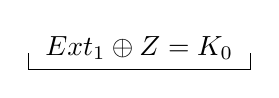
\begin{tikzpicture}
\node[inner xsep=6pt] (identity) {$\operatorname{Ext}_1\oplus Z=K_0$};
\draw ([yshift=6pt]identity.south west) |- (identity.south east) -- ++(0,6pt);
\end{tikzpicture}}\endgroup}
\end{GelfandAdjacentEvidence}
\begin{GelfandAdjacentEvidence}{GELFAND-P000513}{4}

для симплиц. комплексов.
\Unclear{GELFAND-P000513}{ext-operation}{Знак перед $Z$ густо наведён. Условно набран как $\oplus$. Возможно $\otimes$.}
\end{GelfandAdjacentEvidence}
\begin{GelfandAdjacentEvidence}{GELFAND-P000513}{5}


\uline{Пример расширения}.
\[
0\to\mathcal K\to C^*(\text{„}ax+b\text{”})\to C(\infty)\to0
\]
\[
\operatorname{Ext}(\infty)=Z+Z.
\]
Какова эта пара чисел для конкр. опер.?

\begin{center}— · —\end{center}
\sout{\mbox{$X=S^1$}}
\SourceFigure{GELFAND-P000513}{cancelled-torus}{Слева зачёркнуто $X=S^1$.}
\end{GelfandAdjacentEvidence}
\begin{GelfandAdjacentEvidence}{GELFAND-P000513}{6}

\[
X=\mathbb T=S^1
\]
\SourceFigure{GELFAND-P000513}{torus-generator}{%
\begingroup\color{black}\GelfandFitDiagram{\begin{tikzpicture}
\node (circle) at (0,0) {$C(\mathbb T)$};
\node (quotient) at (2.7,0) {$\mathcal L/\mathcal K$};
\draw[->] (circle.east) -- (quotient.west);
\node[anchor=north west,align=left] at (circle.south west)
  {порожд. $z$\\как алг. с инвол.};
\end{tikzpicture}}\endgroup}
\end{GelfandAdjacentEvidence}
\begin{GelfandAdjacentEvidence}{GELFAND-P000513}{7}


Пусть $T$ — образ $z$.
\[
TT^*=1\bmod\mathcal K
\]
\uwave{с точн. до унит. эквив. и \mbox{$\bmod\ 1+\mathcal K$}.}

\uline{Ответ:}\quad\uuline{индекс}\quad(классифик.).

\begin{center}— · —\end{center}
\uline{Теор.}
\[
\left\{\underset{\substack{\vert\\\text{норм.}}}{N}+\mathcal K\right\}
\]
— замкн. по норме во всех опер.,
\SourceFigure{GELFAND-P000513}{normal-pointer}{Под $N$ подпись «норм.» соединена с буквой коротким штрихом.}
\end{GelfandAdjacentEvidence}
\begin{GelfandAdjacentEvidence}{GELFAND-P000513}{8}


а \sout{\mbox{$N_1N_2=N_2N_1$}}
пары $\{N_1+K_1,\ N_2+K_2\}$ с усл. $N_1N_2=N_2N_1$
[вставлено слева в обводке: незамкнуто] в мн-ве всех пар такого вида.
\SourceFigure{GELFAND-P000513}{pair-revisions}{Равенство зачёркнуто перед «пары». Слева обведённая вставка.}
\end{GelfandAdjacentEvidence}
\begin{GelfandAdjacentEvidence}{GELFAND-P000513}{9}

\Unclear{GELFAND-P000513}{cancelled-notclosed}{Под обводкой зачёркнуто слово, условно прочитанное «незамкнуто».}
\end{GelfandAdjacentEvidence}


\uuline{След. раз:}\quad\uwave{докл. Фукса;}\quad\uwave{предст. по Мищенко}.

\uuline{Фукс.}\qquad\uline{Quillen}\qquad\uwave{Higher algebraic K-theory I}

(Proc. of symp. on $K$-theory)

\uline{Introduction.} $M$ — категория (абелева либо спец. аддитивная).
Определяются $K_i(M)$.

\uline{Построения}

$QM$ — катег. частных $\Rightarrow$ классиф. пр-во $BQM$ $\Rightarrow$
\[
\Rightarrow\quad K_i(M)=\pi_{i+1}(BQM).
\]

\uline{Essential part.}

Симпл. объект в категории $S$ — контравар. функтор $\mathrm{Ord}\to S$,
где $\mathrm{Ord}$ — кан. категория из неотриц. целых чисел.


\Needspace{7\baselineskip}
\begin{GelfandAdjacentEvidence}{GELFAND-P000514}{1}
\SourcePage{GELFAND-P000514}{unlabelled}
\[
\mathrm{Ord}^{\circ}\longrightarrow S
\]
\Unclear{GELFAND-P000514}{top-functor}{Над $\mathrm{Ord}$ стоит маленький овал. Условно набран как $\circ$. Возможны $o$ и $0$.}
\end{GelfandAdjacentEvidence}
\begin{GelfandAdjacentEvidence}{GELFAND-P000514}{2}


(Функтор всегда означает ковар. функтор).

$\mathrm{Ord}$\quad объекты — $0,1,2,3,\ldots$

Морф. [зачёркнуто:
\Incomplete{GELFAND-P000514}{upper-cancellation}{Чтение зачёркнутой записи не установлено.}
\end{GelfandAdjacentEvidence}
\begin{GelfandAdjacentEvidence}{GELFAND-P000514}{3}
]
$p\to q$ наз. монотонно неубыв. отображение
\[
(0,1,\ldots,p)\longrightarrow(0,1,\ldots,q)
\]
Все они предст. в виде композ. морф. 2-х сортов:

\SourceFigure{GELFAND-P000514}{order-maps}{%
\begingroup\color{black}\GelfandFitDiagram{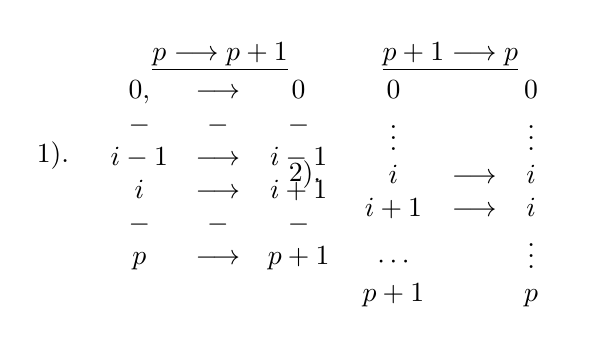
\begin{tikzpicture}
\node[anchor=north west] at (0,0) {$1).\quad
\begin{array}{c}
\underline{p\longrightarrow p+1}\\[2pt]
\begin{array}{@{}ccc@{}}
0,&\longrightarrow&0\\
-&-&-\\
i-1&\longrightarrow&i-1\\
i&\longrightarrow&i+1\\
-&-&-\\
p&\longrightarrow&p+1
\end{array}
\end{array}$};
\node[anchor=north west] at (3.2,0) {$2).\quad
\begin{array}{c}
\underline{p+1\longrightarrow p}\\[2pt]
\begin{array}{@{}ccc@{}}
0&&0\\
\vdots&&\vdots\\
i&\longrightarrow&i\\
i+1&\longrightarrow&i\\
\cdots&&\vdots\\
p+1&&p
\end{array}
\end{array}$};
\end{tikzpicture}}\endgroup}
\end{GelfandAdjacentEvidence}
\begin{GelfandAdjacentEvidence}{GELFAND-P000514}{4}


Для задания симпл. об. дост. указ. посл. объектов
\[
S_0,S_1,S_2,\ldots
\]
и морфизмов
\SourceFigure{GELFAND-P000514}{face-ladder}{%
\begingroup\color{black}\GelfandFitDiagram{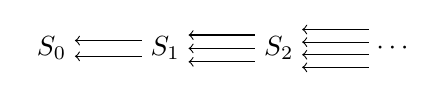
\begin{tikzpicture}[x=.78cm]
\node at (0,0) {$S_0$};
\node at (1.85,0) {$S_1$};
\node at (3.70,0) {$S_2$};
\node at (5.55,0) {$\cdots$};
\foreach \y in {-.10,.10} {\draw[<-] (.38,\y) -- (1.47,\y);}
\foreach \y in {-.17,0,.17} {\draw[<-] (2.23,\y) -- (3.32,\y);}
\foreach \y in {-.24,-.08,.08,.24} {\draw[<-] (4.08,\y) -- (5.16,\y);}
\end{tikzpicture}}\endgroup}
\end{GelfandAdjacentEvidence}
\begin{GelfandAdjacentEvidence}{GELFAND-P000514}{5}

(отвечают вложениям типа 1))

и
\SourceFigure{GELFAND-P000514}{degeneracy-ladder}{%
\begingroup\color{black}\GelfandFitDiagram{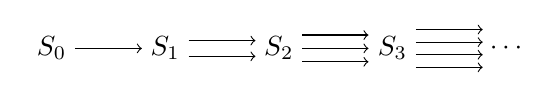
\begin{tikzpicture}[x=.78cm]
\node at (0,0) {$S_0$};
\node at (1.85,0) {$S_1$};
\node at (3.70,0) {$S_2$};
\node at (5.55,0) {$S_3$};
\node at (7.40,0) {$\cdots$};
\draw[->] (.38,0) -- (1.47,0);
\foreach \y in {-.10,.10} {\draw[->] (2.23,\y) -- (3.32,\y);}
\foreach \y in {-.17,0,.17} {\draw[->] (4.08,\y) -- (5.16,\y);}
\foreach \y in {-.24,-.08,.08,.24} {\draw[->] (5.93,\y) -- (7.02,\y);}
\end{tikzpicture}}\endgroup}
\end{GelfandAdjacentEvidence}
\begin{GelfandAdjacentEvidence}{GELFAND-P000514}{6}

(отвеч. отобр. типа 2))

(Соотношения должны быть выполнены).

\hspace*{3em}их легко выписать

$S$ — или кат. мн-в или кат. топ. пр-в.

Но можно: группы; гладк. мн-зия и т.п.

\uuline{Важный пример:} сингу. комплекс топ. пр-ва. $S$ — кат. множеств.

$X$ — топ. пр-во. Обозн. $S_q$ — все сингу. симплексы $X$
\SourceFigure{GELFAND-P000514}{lower-notation}{Сокращение читается «Обозн.».}
\end{GelfandAdjacentEvidence}
\begin{GelfandAdjacentEvidence}{GELFAND-P000514}{7}


(непр. отобр. $\Delta^q\to X$, где
\[
\Delta^q=\{(x_1,\ldots,x_{q+1})\in R^{q+1},\quad x_i\geq0,\quad\sum x_i=1\}.
\]
\SourceFigure{GELFAND-P000514}{singular-parenthesis}{Перед «непр. отобр.» стоит открывающая скобка. Перед следующей формулой парная скобка не видна.}
\end{GelfandAdjacentEvidence}
\begin{GelfandAdjacentEvidence}{GELFAND-P000514}{8}


\[
\exists\ \delta_i:\Delta^{q-1}\longrightarrow\Delta^q
\]
канонич. отобр. на $i$-ю грань (верш. упоряд.)
\Unclear{GELFAND-P000514}{lower-face-symbol}{Буква с индексом $i$ условно набрана как $\delta_i$. Возможно $\gamma_i$.}
\end{GelfandAdjacentEvidence}
\begin{GelfandAdjacentEvidence}{GELFAND-P000514}{9}


Син. симпл. — композиция
\[
\Delta^{q-1}\longrightarrow\Delta^q\longrightarrow X
\]
\Unclear{GELFAND-P000514}{lower-singular-abbreviation}{Начальное сокращение условно прочитано «Син.». Возможна другая последняя буква.}
\end{GelfandAdjacentEvidence}
\begin{GelfandAdjacentEvidence}{GELFAND-P000514}{10}


Получ. $q+1$ отображение
\SourceFigure{GELFAND-P000514}{face-family}{%
\begingroup\color{black}\GelfandFitDiagram{\begin{tikzpicture}
\node at (0,0) {$S_q$};
\node at (2.05,0) {$S_{q-1}$};
\draw[->] (.50,.19) -- (1.45,.19);
\node at (.96,0) {$\cdots$};
\draw[->] (.50,-.19) -- (1.45,-.19);
\node[anchor=west] at (2.52,0) {(грани).};
\end{tikzpicture}}\endgroup}
\end{GelfandAdjacentEvidence}
\begin{GelfandAdjacentEvidence}{GELFAND-P000514}{11}


\SourceFigure{GELFAND-P000514}{degeneracy-family}{%
\begingroup\color{black}\GelfandFitDiagram{\begin{tikzpicture}
\node at (0,0) {$S_q$};
\node at (2.05,0) {$S_{q+1}$};
\draw[->] (.50,.19) -- (1.45,.19);
\node at (.96,0) {$\cdots$};
\draw[->] (.50,-.19) -- (1.45,-.19);
\node[anchor=north] at (.97,-.32) {($q+1$ шт.)};
\end{tikzpicture}}\endgroup}
\end{GelfandAdjacentEvidence}

из $\Delta^{q+1}\longrightarrow\Delta^q$\quad аффинные проекции
($i$-я склеив. $i$-ю верш. с $(i+1)$-й).

\begin{center}— · —\end{center}


\Needspace{7\baselineskip}
\begin{GelfandAdjacentEvidence}{GELFAND-P000515}{1}
\SourcePage{GELFAND-P000515}{15}
\uline{Реализация}.

Пусть $S$ — кат. мн-в или топ. пр-в.

Симпл. об. в кат. мн-в или топ. пр-в относится топ. пр-во.

\uwave{Элементы} [вписано над строкой, в обводке: м-ва] \uwave{\mbox{$S_i$} наз. симплексами}
\SourceFigure{GELFAND-P000515}{set-insertion}{Сокращение «м-ва» в обводке отведено к месту после «Элементы».}
\end{GelfandAdjacentEvidence}
\begin{GelfandAdjacentEvidence}{GELFAND-P000515}{2}


\uwave{Образы стрелок слева направо наз. вырожд. симплексами.}

\uwave{Прочие наз. невырожденными.} \uwave{Стр. справа налево перев. невыр. в невырожденные.}
\SourceFigure{GELFAND-P000515}{nondegenerate-faces}{Рукописная строка читается «Стр. справа налево перев. невыр. в невырожденные».}
\end{GelfandAdjacentEvidence}
\begin{GelfandAdjacentEvidence}{GELFAND-P000515}{3}


Рассм. $\Delta^q\times S_q^0$

\hspace*{3em}невыр. симп. из $S_q$.\qquad ($S_q^0$ — дискр. топ. пр-во).

В $\coprod_q\Delta^q\times S_q^0$ (несвязн. объединение) отождествление.
\[
\Delta^{q-1}\times s,\qquad s\in S_{q-1}^0
\]
отожд. с частью $\Delta^q\times s'$, $s'\in S_q^0$,
когда $s$ — образ $s'$ при отобр. ($i$-м)
\[
S_{q-1}\overset{i}{\longleftarrow}S_q\qquad
\text{($i$-я грань)}
\]
\SourceFigure{GELFAND-P000515}{gluing-membership}{В условии принадлежности после $s$ виден штрих: $s'\in S_q^0$.}
\end{GelfandAdjacentEvidence}
\begin{GelfandAdjacentEvidence}{GELFAND-P000515}{4}


\uline{Получ. топ. пр-во.} \uline{Это клеточное пр-во} (не склеив. внутренности).

Но: точки границы могут склеиться (так что не симплиц. пр-во).

То же прим., если $S$ — топ. пр-ва. Уже не возникает топ. структ.,
т.к. в $\Delta^q\times S_q^0$ топ. прямого произв.
\SourceFigure{GELFAND-P000515}{topological-wording}{Рукописная строка читается «Уже не возникает топ. структ.».}
\end{GelfandAdjacentEvidence}
\begin{GelfandAdjacentEvidence}{GELFAND-P000515}{5}


\uuline{Упр.:} для хорошего топ. пр-ва реализация сингу.
[зачёркнуто: \Incomplete{GELFAND-P000515}{middle-cancellation}{Чтение под зачёркиванием не установлено.}
\end{GelfandAdjacentEvidence}
\begin{GelfandAdjacentEvidence}{GELFAND-P000515}{6}
]
комплекса гомотоп. эквив. $X$.

Для восстан. полиэдра надо принять за $S_i$ афф. отобр. симплексов туда
\SourceFigure{GELFAND-P000515}{polyhedron-abbreviation}{Сокращение перед «полиэдра» читается «восстан.».}
\end{GelfandAdjacentEvidence}
\begin{GelfandAdjacentEvidence}{GELFAND-P000515}{7}

\SourceFigure{GELFAND-P000515}{polyhedron-sketch}{%
\begingroup\color{black}\GelfandFitDiagram{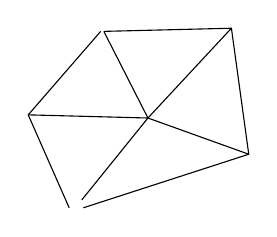
\begin{tikzpicture}[x=.02cm,y=-.02cm]
\draw (64,25)--(145,23)--(156,103)--(51,137);
\draw (42,137)--(16,78)--(62,25);
\draw (92,80)--(64,25);
\draw (92,80)--(145,23);
\draw (92,80)--(156,103);
\draw (92,80)--(50,132);
\draw (92,80)--(16,78);
\end{tikzpicture}}\endgroup}
\end{GelfandAdjacentEvidence}
\begin{GelfandAdjacentEvidence}{GELFAND-P000515}{8}


\uwave{Реализация коммут. с умножением.}
\SourceFigure{GELFAND-P000515}{product-diagrams}{%
\begingroup\color{black}\GelfandFitDiagram{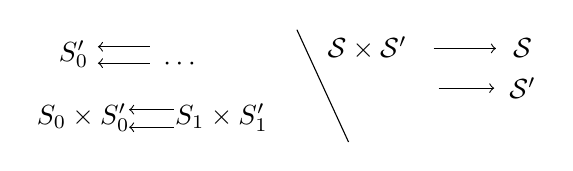
\begin{tikzpicture}[x=.72cm,y=.72cm]
\node at (.25,0) {$S'_0$};
\node at (2.12,-.18) {$\cdots$};
\draw[<-] (.68,.13) -- (1.60,.13);
\draw[<-] (.68,-.16) -- (1.60,-.16);
\node at (.42,-1.12) {$S_0\times S'_0$};
\node at (2.86,-1.12) {$S_1\times S'_1$};
\draw[<-] (1.23,-.98) -- (2.02,-.98);
\draw[<-] (1.23,-1.29) -- (2.02,-1.29);
\draw (4.19,.43) -- (5.10,-1.55);
\node at (5.43,.10) {$\mathcal S\times\mathcal S'$};
\node at (8.17,.10) {$\mathcal S$};
\node at (8.17,-.60) {$\mathcal S'$};
\draw[->] (6.60,.10) -- (7.70,.10);
\draw[->] (6.69,-.60) -- (7.67,-.60);
\end{tikzpicture}}\endgroup}
\end{GelfandAdjacentEvidence}
\begin{GelfandAdjacentEvidence}{GELFAND-P000515}{9}


отсюда
\SourceFigure{GELFAND-P000515}{realization-projections}{%
\begingroup\color{black}\GelfandFitDiagram{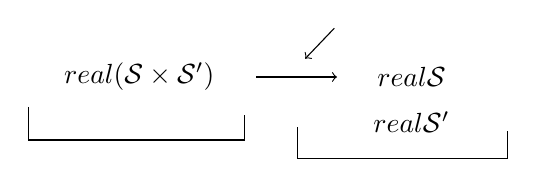
\begin{tikzpicture}[x=.86cm,y=.86cm]
\node at (1.65,0) {$\operatorname{real}(\mathcal S\times\mathcal S')$};
\node at (5.67,0) {$\operatorname{real}\mathcal S$};
\node at (5.67,-.66) {$\operatorname{real}\mathcal S'$};
\draw[->] (3.38,0) -- (4.57,0);
\draw[->] (4.53,.72) -- (4.10,.27);
\draw (.01,-.44) -- (.01,-.93) -- (3.20,-.93) -- (3.20,-.56);
\draw (3.98,-.74) -- (3.98,-1.20) -- (7.09,-1.20) -- (7.09,-.80);
\end{tikzpicture}}\endgroup}
\end{GelfandAdjacentEvidence}
\begin{GelfandAdjacentEvidence}{GELFAND-P000515}{10}


и они составляют
\SourceFigure{GELFAND-P000515}{realization-product-map}{%
\begingroup\color{black}\GelfandFitDiagram{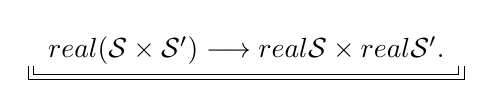
\begin{tikzpicture}
\node[inner xsep=5pt] (product) {$\operatorname{real}(\mathcal S\times\mathcal S')
 \longrightarrow\operatorname{real}\mathcal S\times\operatorname{real}\mathcal S'.$};
\draw ([yshift=3pt]product.south west) |- (product.south east) -- ++(0,3pt);
\draw ([xshift=-2pt,yshift=3pt]product.south west) |-
 ([xshift=2pt,yshift=-2pt]product.south east) -- ++(0,5pt);
\end{tikzpicture}}\endgroup}
\end{GelfandAdjacentEvidence}
\begin{GelfandAdjacentEvidence}{GELFAND-P000515}{11}


\uuline{Утв.} \uwave{Оказ., что оно} — \uuline{гомеоморфизм.}

\uline{Пример.}
\SourceFigure{GELFAND-P000515}{ordered-segment}{%
\begingroup\color{black}\GelfandFitDiagram{\begin{tikzpicture}
\draw (0,0)--(1.2,0);
\draw (0,-.10)--(0,.10);
\draw (1.2,-.10)--(1.2,.10);
\end{tikzpicture}}\endgroup\quad Упор. отрезок.}
\end{GelfandAdjacentEvidence}
\begin{GelfandAdjacentEvidence}{GELFAND-P000515}{12}


$S^0$ — 2 элемента

$S^1$ — 3 элем. (с учётом вырожд.)

$S^p=(p+2)$ элем. $i$-й:
\[
[0,i-1]\longrightarrow0,\qquad[i,p]\longrightarrow1
\]
\Unclear{GELFAND-P000515}{lower-overwritten-exponent}{Верхний знак справа от $S$ густо наведён. Условно набран как $p$. Слева над $S$ виден короткий штрих.}
\end{GelfandAdjacentEvidence}
\begin{GelfandAdjacentEvidence}{GELFAND-P000515}{13}


$S_p\times S_p$
\Unclear{GELFAND-P000515}{product-foot-marks}{Правее произведения видны отдельные слабые штрихи. Чтение не установлено.}
\end{GelfandAdjacentEvidence}


(в следующий раз.)


\Needspace{7\baselineskip}
\begin{GelfandAdjacentEvidence}{GELFAND-P000516}{1}
\SourcePage{GELFAND-P000516}{unlabelled}
\S2. \uline{Классиф. пр-во в категории.}

$C$ — категория (малая). С ней связ. её нерв $NC$ (симпл. объект кат. множеств).
\[
NC_q=\{\text{[?]}\quad X_0\longrightarrow\cdots\longrightarrow X_q\}
\qquad\text{мн-во таких диаграмм}
\]
\Unclear{GELFAND-P000516}{nerve-blot}{После открывающей фигурной скобки перед $X_0$ виден густо переписанный знак. Чтение не установлено.}
\end{GelfandAdjacentEvidence}
\begin{GelfandAdjacentEvidence}{GELFAND-P000516}{2}


\[
\underline{NC_q\longrightarrow NC_{q-1}}
\]

\uline{0-е}
\SourceFigure{GELFAND-P000516}{discard-face}{%
\begingroup\color{black}\GelfandFitDiagram{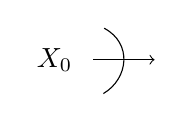
\begin{tikzpicture}[baseline=(object.base)]
\node (object) at (0,0) {$X_0$};
\draw[->] (.49,0) -- (1.27,0);
\draw (.63,.40) .. controls (.99,.21) and (.94,-.24) .. (.62,-.43);
\end{tikzpicture}}\endgroup\qquad (отбросим).}
\end{GelfandAdjacentEvidence}
\begin{GelfandAdjacentEvidence}{GELFAND-P000516}{3}


\uline{\mbox{$q$}-е} — отбрас. $X_q$

\uuline{\mbox{$i$}-е} — композ. $i$ и \mbox{$i+1$}-й стрелок
\SourceFigure{GELFAND-P000516}{composition-face}{%
\begingroup\color{black}\GelfandFitDiagram{\begin{tikzpicture}
\node at (0,0) {$\cdots$};
\node at (1.47,0) {$X_i$};
\node at (3.1,0) {$\cdots$};
\draw[->] (.29,0) -- (1.08,0);
\draw[->] (1.83,0) -- (2.63,0);
\draw[->] (.20,-.25) .. controls (.72,-.80) and (2.04,-.72) .. (2.74,-.23);
\end{tikzpicture}}\endgroup}
\end{GelfandAdjacentEvidence}
\begin{GelfandAdjacentEvidence}{GELFAND-P000516}{4}


\[
\underline{NC_q\longrightarrow NC_{q+1}}
\]
один из $X$ раздваивается и вставл. тожд. морфизм.

\uline{\sout{Нерв.}}\qquad
$\operatorname{Real}NC=BC$ — классиф. пр-во категории.
\Unclear{GELFAND-P000516}{definition-cancellation}{Зачёркнутое слово условно прочитано «Нерв.».}
\end{GelfandAdjacentEvidence}
\begin{GelfandAdjacentEvidence}{GELFAND-P000516}{5}


\uline{Пример:} классиф. пр-во группы $G$ получ. из след. катег.:
\Incomplete{GELFAND-P000516}{group-cancellation}{Чтение под зачёркиванием после двоеточия не установлено.}
\end{GelfandAdjacentEvidence}
\begin{GelfandAdjacentEvidence}{GELFAND-P000516}{6}

\SourceFigure{GELFAND-P000516}{group-category-abbreviation}{После «из» написано «след. катег.».}
\end{GelfandAdjacentEvidence}
\begin{GelfandAdjacentEvidence}{GELFAND-P000516}{7}


1 объект, а морфизмы — \uwave{Элементы \mbox{$G$}.}
\[
NC_q=\underbrace{G\times\cdots\times G}_{q}
\]

\begin{center}— · —\end{center}
$G=Z_2$. Симплексы:

\uwave{Невыр. симп.} — не содержат 1.

По 1 невыр. симп. каждой размерности.

\SourceFigure{GELFAND-P000516}{exercise-margin-mark}{%
\begingroup\color{black}\GelfandFitDiagram{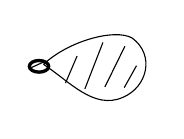
\begin{tikzpicture}[x=.82cm,y=.82cm]
\draw (-.72,.08) .. controls (-.34,.44) and (.38,.64) .. (.65,.49)
  .. controls (1.01,.23) and (.89,-.27) .. (.51,-.43)
  .. controls (.06,-.63) and (-.32,-.18) .. (-.72,.08);
\draw (-.38,-.21) -- (-.20,.21);
\draw (-.08,-.30) -- (.20,.42);
\draw (.23,-.27) -- (.54,.36);
\draw (.53,-.28) -- (.72,.06);
\draw[very thick] (-.79,.05) ellipse (.15 and .09);
\draw (-.91,.03) -- (-.69,.13);
\end{tikzpicture}}\endgroup\par\smallskip Три длинных и один короткий штрих в овале. У левого края тёмное наложение.}
\end{GelfandAdjacentEvidence}
\begin{GelfandAdjacentEvidence}{GELFAND-P000516}{8}

Упр. 2-мерную намот. дважды. Получается $RP_{\infty}$.
\SourceFigure{GELFAND-P000516}{exercise-phrase}{Рукописная фраза читается «2-мерную намот. дважды».}
\end{GelfandAdjacentEvidence}
\begin{GelfandAdjacentEvidence}{GELFAND-P000516}{9}

\SourceFigure{GELFAND-P000516}{exercise-word}{В конце фразы написано «дважды».}
\end{GelfandAdjacentEvidence}
\begin{GelfandAdjacentEvidence}{GELFAND-P000516}{10}


\begin{center}— · —\end{center}
Пусть $M$ — категория, к-рая либо абелева, либо полная подкат. абелевой кат., замкн. отн. взятия расширений. Пусть классы изом. объектов сост. множество. Тогда она эквивалентна малой категории.
\uwave{Категория \mbox{$QM$}.}\quad
$\underline{\operatorname{Ob}(QM)=\operatorname{Ob}(M)}$.

\[
\operatorname{Hom}_{QM}(X',X'')\ \Rightarrow\ \text{диаграммы}
\]
\SourceFigure{GELFAND-P000516}{q-span}{%
\begingroup\color{black}\GelfandFitDiagram{\begin{tikzpicture}
\node at (0,0) {$X'$};
\node at (2.12,0) {$X$};
\node at (3.75,0) {$X''$};
\draw[<-] (.31,0) -- (1.82,0);
\draw[->] (2.42,0) -- (3.41,0);
\draw[->] (.85,-.85) -- (1.25,-.23);
\draw[->] (4.05,-1.04) .. controls (3.41,-.86) and (3.01,-.54) .. (2.93,-.23);
\node[align=left,anchor=north west] at (-.32,-.87) {эпиморфизм\\с ядром};
\node[align=left,anchor=north west] at (3.65,-1.12) {мономорфизм\\с коядром};
\end{tikzpicture}}\endgroup}
\end{GelfandAdjacentEvidence}
\begin{GelfandAdjacentEvidence}{GELFAND-P000516}{11}


Это категория.

\uline{Определение.}
\SourceFigure{GELFAND-P000516}{k-definition}{%
\begingroup\color{black}\GelfandFitDiagram{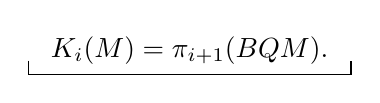
\begin{tikzpicture}
\node[inner xsep=8pt] (formula) {$K_i(M)=\pi_{i+1}(BQM).$};
\draw ([yshift=5pt]formula.south west) |- (formula.south east) -- ++(0,5pt);
\end{tikzpicture}}\endgroup}
\end{GelfandAdjacentEvidence}



\Needspace{7\baselineskip}
\begin{GelfandAdjacentEvidence}{GELFAND-P000517}{1}
\SourcePage{GELFAND-P000517}{unlabelled}
\uline{Продолжение докл. Фукса} (по Марченко).

\uwave{Пример реализации}

$S_q$ состоит из $q+2$ элементов. Интерпр. его как мн-во афф. отобр.
$\Delta^q$ в отрезок $\Delta^1$, согласованных с упорядочением вершин $\Delta^q$ и $\Delta^1$.

Морфизмы $S_{q-1}\leftarrow S_q\to S_{q+1}$ опр. как для сингулярных симплексов пр-ва
$I=\Delta^1$ [вписано над строкой: (сужение на аффинные)], т. е. композицией с вложением и ограничениями.
\SourceFigure{GELFAND-P000517}{affine-insertion}{Вставка «сужение на аффинные» обведена и отведена к месту после формулы.}
\end{GelfandAdjacentEvidence}
\begin{GelfandAdjacentEvidence}{GELFAND-P000517}{2}


Невырожд. симплексы — 2 0-мерных $*\to I$ и 1 одномерный.

$S_q\times S_q$\qquad когда элемент $S_q\times S_q$ невыр.?

Элм. — пара $(\varphi,\psi)$, он невыр., когда нет 2-х вершин в $\Delta^q$,
отображающихся $\varphi$ и $\psi$ [зачёркнуто:
\Incomplete{GELFAND-P000517}{cancelled-sign}{Чтение знака под зачёркиванием не установлено.}
\end{GelfandAdjacentEvidence}
\begin{GelfandAdjacentEvidence}{GELFAND-P000517}{3}
]
в одну [зачёркнуто:
\Incomplete{GELFAND-P000517}{cancelled-word}{Чтение слова под зачёркиванием не установлено.}
\end{GelfandAdjacentEvidence}
\begin{GelfandAdjacentEvidence}{GELFAND-P000517}{4}
] вершину.

\[
S_0\times S_0\quad\text{— 4 элм.}\qquad *\to(0,0),(0,1),(1,0),(1,1)
\]
\[
\begin{gathered}
S_1\times S_1\qquad
\binom{1}{0}\to
\begin{matrix}\varphi&\psi\\0&0\\0&1\end{matrix}
\qquad
\left(\begin{matrix}0&1\\0&1\end{matrix}\ \text{вырожден}\right)\\
\begin{pmatrix}0&0\\1&1\end{pmatrix}
\begin{pmatrix}0&0\\1&0\end{pmatrix}
\begin{pmatrix}0&1\\1&1\end{pmatrix}
\begin{pmatrix}1&0\\1&1\end{pmatrix}
\end{gathered}
\]
\Unclear{GELFAND-P000517}{array-cancellation}{После второго столбца перед «вырожден» зачёркнут штрих, похожий на закрывающую скобку.}
\end{GelfandAdjacentEvidence}
\begin{GelfandAdjacentEvidence}{GELFAND-P000517}{5}

\[
S_2\times S_2\qquad \Delta\to
\begin{matrix}0&0&0&0\\1&0&0&1\\1&1&1&1\end{matrix}
\]
\SourceFigure{GELFAND-P000517}{double-array}{В рукописи четыре столбца без разделителей.}
\end{GelfandAdjacentEvidence}
\begin{GelfandAdjacentEvidence}{GELFAND-P000517}{6}


Реализация $S\times S$.
\SourceFigure{GELFAND-P000517}{realization-square}{%
\begingroup\color{black}\GelfandFitDiagram{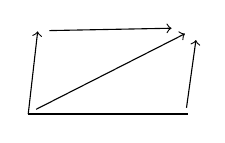
\begin{tikzpicture}
\draw[->] (0,0) -- (.12,1.05);
\draw[->] (.27,1.06) -- (1.82,1.09);
\draw[->] (2.01,.08) -- (2.13,.94);
\draw[->] (.10,.06) -- (1.99,1.02);
\draw (0,0) -- (2.03,0);
\end{tikzpicture}}\endgroup\par\smallskip У правого конца нижней стороны штрихи наложены друг на друга. Направление этой стороны не установлено.}
\end{GelfandAdjacentEvidence}
\begin{GelfandAdjacentEvidence}{GELFAND-P000517}{7}


\uline{Классиф. пр-во категории.}

$C$ — малая кат., $NC$ — нерв категории

$(NC)_q\ (=S_q)$ — все диагр. $C$ вида $X_0\to\ldots\to X_q$

отобр. — взятие композ., отбрс. концов и вставление $\mathrm{id}\,X_j$.
\Unclear{GELFAND-P000517}{endpoint-abbreviation}{Сокращение перед «концов» условно прочитано «отбрс.». Возможно «отброс.».}
\end{GelfandAdjacentEvidence}
\begin{GelfandAdjacentEvidence}{GELFAND-P000517}{8}

\Unclear{GELFAND-P000517}{identity-index}{Индекс у $X$ условно набран как $j$. Возможна прописная $J$.}
\end{GelfandAdjacentEvidence}
\begin{GelfandAdjacentEvidence}{GELFAND-P000517}{9}

\[
BC=\mathrm{Real}\,NC.
\]
Вершины $BC$ — объекты $C$, 1-мерные симплексы — нетождественные морфизмы.
$\Delta$ натягиваются на коммутативные симплексы
\SourceFigure{GELFAND-P000517}{commutative-triangle}{%
\begingroup\color{black}\GelfandFitDiagram{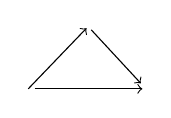
\begin{tikzpicture}
\draw[->] (0,0) -- (.74,.77);
\draw[->] (.80,.75) -- (1.43,.07);
\draw[->] (.08,0) -- (1.45,0);
\end{tikzpicture}}\endgroup}
\end{GelfandAdjacentEvidence}
\begin{GelfandAdjacentEvidence}{GELFAND-P000517}{10}

и т. д.

Барицентрич. подразд. полиэдра высокой степ. — нерв нек-рой категории.
\Unclear{GELFAND-P000517}{subdivision-abbreviation}{Сокращение условно прочитано «подразд.». Последняя буква может читаться как «б».}
\end{GelfandAdjacentEvidence}


\uline{Св-ва:}
\[
B(C\times C')\cong BC\times BC'
\]
\[
f:C\rightsquigarrow C'\quad\Rightarrow\quad Bf:BC\to BC'
\]
Если есть ещё $g:C\to C'$ и естеств. отобр. $f$ в $g$, то
$Bg:BC\to BC'$ связывается с $Bf$ канонической гомотопией.

Пусть $\{0,1\}$ — кат. из 2-х объектов с одним морфизмом $0\to1$

Морфизм функторов $f$ и $g$ — функтор из $C\times\{0,1\}$ в $C'$.


\Needspace{7\baselineskip}
\begin{GelfandAdjacentEvidence}{GELFAND-P000518}{1}
\SourcePage{GELFAND-P000518}{21}
$F:C\times\{0,1\}\to C'$. На концах $f,g$; морф. $0,1$ — естеств. отобр.

Он определяет отобр. — гомотопию, связывающую $f$ с $g$
\[
BC\times I=B(C\times I)\to BC'.
\]

Если $C$ имеет финальный или начальный объект, то $BC$ стягиваемо —\\
— оно конус.

Если $f:C\rightsquigarrow C'$ имеет левый или правый сопряженный, то $Bf$ — гомотопическая эквивалентность.
\[
BC^{\circ}=BC,\qquad B(C\times C')=BC\times BC'.
\]

\uline{Аналог гомотопич. послед. расслоения.}

Пусть $f:X\to Y$ — рассл. Серра. Тогда
\[
\begin{aligned}
\ldots\to\pi_q(X,x)\to\pi_q(Y,f(x))
&\to\pi_{q-1}(f^{-1}(f(x),x)\\
&\to\pi_{q-1}(X,x)\to\ldots
\end{aligned}
\]
\SourceFigure{GELFAND-P000518}{fibre-parentheses}{Скобки набраны как в рукописи. Перед запятой видна одна закрывающая скобка.}
\end{GelfandAdjacentEvidence}
\begin{GelfandAdjacentEvidence}{GELFAND-P000518}{2}


Если $f$ не уд. акс. о накр. гомот., то после замены на эквив. будет ей удовл. и получим послед. Вот конструкция:

Пусть $\widetilde X=\{(x,s),\ x\in X,\ s:I\to Y,\ s(0)=f(x)\}$.

$\widetilde X\underset{\sim}{\supset}X$. Отобр. $\widetilde f:\widetilde X\to Y$ строится так:

$\widetilde f(x,s)=s(1),\qquad\widetilde f|_X=f$ но уже есть акс. накр. гом.

Из-за $\widetilde X\simeq X$ имеем точную послед.
\Unclear{GELFAND-P000518}{homotopy-relation}{Знак между $\widetilde X$ и $X$ условно набран как $\simeq$. В рукописи волнистый и прямой штрихи пересекаются.}
\end{GelfandAdjacentEvidence}
\begin{GelfandAdjacentEvidence}{GELFAND-P000518}{3}

\[
\ldots\to\pi_q(X)\to\pi_q(Y)\to
\pi_{q-1}(\text{гомот. слой})\to\pi_{q-1}(X)\to\ldots
\]

Пусть теперь \underline{$g:C\rightsquigarrow C'$}, тогда есть

$Bg:BC\rightsquigarrow BC'$. Хочется постр. «гомотопич. слой» $Bg$.

Это не сделано, есть суррогат.

Констр. зависит ещё от нек. объекта $Y\in\mathrm{Ob}\,C'$.

Опр. категорию $Y\backslash g$. $\mathrm{Ob}(Y\backslash g)$ — пары $(X,u)$, где
\[
X\in\mathrm{Ob}\,C,\qquad u\in\mathrm{Mor}_{C'}(Y,g(x)).
\]

Морфизм $(X,u)$ в $(X',u')$ — морфизм $\varphi:X\to X'$,
соглас. с $u$ и $u'$. Есть естеств. отображение
\[
B(Y\backslash g)\to\text{гомот. слой }Bg:BC\to BC'
\]
\SourceFigure{GELFAND-P000518}{object-case}{В аргументе $g(x)$ виден строчный $x$. В парах при описании морфизма буквы читаются как прописные $X$ и $X'$.}
\end{GelfandAdjacentEvidence}


\uline{Теорема}. Пусть функтор $g$ таков, что

$\forall v\in\mathrm{Mor}_{C'}(Y,Y')$ возникающее отображение
$Y'\backslash g\overset{v\backslash g}{\longrightarrow}Y\backslash g$
и $B(v\backslash g):B(Y'\backslash g)\to B(Y\backslash g)$ явл. гомот. эквивал.
(что, вообще говоря, неверно). Тогда $B(Y\backslash g)$ — гомот. слой
$BC\overset{Bg}{\rightsquigarrow}BC'$.


\Needspace{7\baselineskip}
\begin{GelfandAdjacentEvidence}{GELFAND-P000519}{1}
\SourcePage{GELFAND-P000519}{unlabelled}
Постр. отобр. $B(Y\backslash g)$ — гомот. слой $Bg$.

Если есть $(X_0,u_0)\leftarrow\cdots\leftarrow(X_\tau,u_\tau)$
(симплекс $B(Y\backslash g)$)
то есть и $X_0\leftarrow\cdots\leftarrow X_\tau$
и нужно знать лишь $Y\to g(X_\tau)$ (по нему восстанавливаются все $u_j$
\SourceFigure{GELFAND-P000519}{unclosed-parenthesis}{В рукописи после этой строки нет закрывающей скобки.}
\end{GelfandAdjacentEvidence}
\begin{GelfandAdjacentEvidence}{GELFAND-P000519}{2}


$X_0\leftarrow\cdots\leftarrow X_\tau$ — симплекс $BC$ размерности $\tau$.
Вместе с $u_\tau$ он опред. симплекс
\[
g(X_0)\leftarrow\cdots\leftarrow g(X_\tau)\overset{u}{\leftarrow}Y
\]
в $BC'$.
\Unclear{GELFAND-P000519}{simplex-index}{Индекс условно набран как $\tau$. Так же набрана буква в обозначениях размерностей.}
\end{GelfandAdjacentEvidence}
\begin{GelfandAdjacentEvidence}{GELFAND-P000519}{3}


Таким обр., по симплексу в $B(Y\backslash g)$ мы определили 2 симплекса — в $BC$ и в $BC'$
размерностей $\tau$ и $\tau+1$ соотв..
Симпл. из $B(Y\backslash g)$ отобр. так: точка пр-ва $BC$
соотв. этой точке (в барицентр. координ.) и прямой путь в симплексе $BC'$, соединяющий $Bg$ от этой точки в $Y$:
\SourceFigure{GELFAND-P000519}{simplex-sketch}{%
\begingroup\color{black}\GelfandFitDiagram{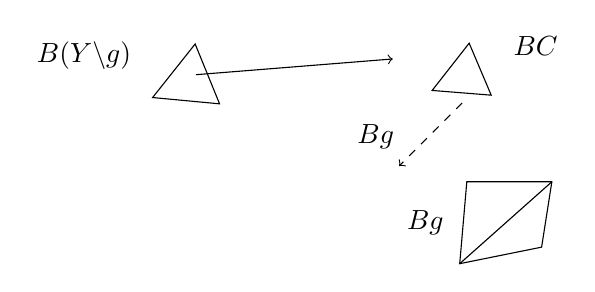
\begin{tikzpicture}[x=1cm,y=1cm]
\node[anchor=east] at (-.15,1.08) {$B(Y\backslash g)$};
\draw (0,.55) -- (.54,1.23) -- (.85,.47) -- cycle;
\draw[->] (.55,.84) -- (3.05,1.04);
\draw (3.55,.64) -- (4.02,1.24) -- (4.30,.58) -- cycle;
\node[anchor=west] at (4.46,1.2) {$BC$};
\draw[dashed,->] (3.93,.48) -- (3.13,-.32);
\node[anchor=east] at (3.19,.05) {$Bg$};
\draw (3.90,-1.56) -- (3.99,-.52) -- (5.07,-.52) -- (4.94,-1.35) -- cycle;
\draw (3.90,-1.56) -- (5.07,-.52);
\node[anchor=east] at (3.82,-1.04) {$Bg$};
\end{tikzpicture}}\endgroup\par\smallskip У левой стороны четырёхугольника после $Bg$ видны наложенные штрихи. Их чтение не установлено.}
\end{GelfandAdjacentEvidence}
\begin{GelfandAdjacentEvidence}{GELFAND-P000519}{4}


Это гомот. экв. $\forall v$ iff вып. условия теоремы.
\SourceFigure{GELFAND-P000519}{sketch-quantifier}{В начале второй строки справа от рисунка читается $\forall v$.}
\end{GelfandAdjacentEvidence}
\begin{GelfandAdjacentEvidence}{GELFAND-P000519}{5}


\uline{Замеч. Фукса}: вероятно $Y\backslash g$ надо опр. как обр. пред. по спектру всех
\underline{$Y\backslash g$} \uline{с р}азличными $Y$.

\uuline{Мищенко.} (\uwave{Представления по Мищенко})

$\Lambda$ — кольцо с инволюцией, $H$ — гильбертово пр-во и 2 предст.
$T_1$ и $T_2$ кольца $\Lambda$ в алгебру огр. опер. в $H$, $F$ — фредгольмов оператор в $H$ и пусть
\[
\forall\lambda\in\Lambda\qquad FT_1(\lambda)-T_2(\lambda)F\in\operatorname{Comp}(H)
\]
Эта система $\{T_1,T_2,F\}$ наз. фредгольмовым предст. $\Lambda$.

Атья рассматривал $\Lambda=C(M)$, $M$ — многообразие (симпозиум в Токио).
\SourceFigure{GELFAND-P000519}{atiyah-parenthesis}{Чтение скобочной записи «симпозиум в Токио».}
\end{GelfandAdjacentEvidence}
\begin{GelfandAdjacentEvidence}{GELFAND-P000519}{6}


\uline{Констр. с этими пред}ставлениями

1) Атья (1970) $\Lambda=C(M)$\qquad
$\forall$ предст. сопост. $\operatorname{index}T\in K_0(M)$

2) $\Lambda=\mathbb Z[\pi]\quad\Rightarrow\quad\forall$ предст. строится
$\xi_T\in K^0(B\pi)$.

3) $\Lambda$ — любое,\qquad
$A=(a_{ij})$ — квадр. форма на $\Lambda^n$\quad $(a_{ij}\in\Lambda)$
\[
A^*=A,\quad\exists A^{-1}\quad\Rightarrow\quad
\text{Строится }\operatorname{sign}_T A\in\mathbb Z.
\]

\Incomplete{GELFAND-P000519}{cancelled-number}{Зачёркнутый номер перед «1)». Возможно «4)».}
\end{GelfandAdjacentEvidence}
\begin{GelfandAdjacentEvidence}{GELFAND-P000519}{7}

1) $\Lambda=C(M)$, $T$ — фредг. предст. $\Lambda$ в $H$,\quad $T=(T_1,T_2,F)$.

$H_i$ — модули над $\Lambda$.\qquad $\operatorname{ind}F$ — число.
Пусть $\eta$ — расслоение,
$\Gamma(\eta)$ — проект. модуль над $C(M)$. Рассмотрим
\end{GelfandAdjacentEvidence}



\Needspace{7\baselineskip}
\begin{GelfandAdjacentEvidence}{GELFAND-P000520}{1}
\SourcePage{GELFAND-P000520}{22}
\[
H_1\otimes_{C(M)}\Gamma(\eta)
\overset{F\otimes 1_\eta}{\longrightarrow}
H_2\otimes_{C(M)}\Gamma(\eta)
\]
\[
\operatorname{ind}(F\otimes1_\eta):K^0(M)\to\mathbb Z,
\quad\text{т.е. элемент }K_0(M)
\]
Это грубовато из-за $\exists$ элем. конечного порядка в $K^0(M)$.

Точнее: $T$ опред. $\operatorname{index}_T:K^0(M\times Y)\to K^0(Y)$;\quad $\forall Y$.
Это уже элемент из $K_0(M)$.

Если $\sigma(A)\in K^0(T^*M)$,\quad $A:H\to H$,\quad т.к. $[f,A]$ —
комп., то есть
\Incomplete{GELFAND-P000520}{cancelled-before-index}{Короткая зачёркнутая группа знаков перед «index» не читается.}
\end{GelfandAdjacentEvidence}
\begin{GelfandAdjacentEvidence}{GELFAND-P000520}{2}

$\operatorname{index}(A)\in K_0(M)$.
\Unclear{GELFAND-P000520}{commutator-connector}{Штрих после коммутатора обведён. Он условно набран как тире.}
\end{GelfandAdjacentEvidence}
\begin{GelfandAdjacentEvidence}{GELFAND-P000520}{3}

Так. эти элем. двойств. друг другу по Пуанкаре
$K^0(T^*M)\underset{\mathcal D}{\sim}K_0(M)$.
Тогда $\operatorname{index}A=\mathcal D(\sigma(A))$

(NB можно стр. \uline{прямой} образ $A$)

2) $\pi$ — произв. дискр. группа, $\Lambda=\mathbb Z[\pi]$ — её групп. кольцо, $B_\pi$ —\\
— классиф. пр-во. $T$ — фредг. предст.: $T=(T_1,F,T_2)$. Надо постр.
$\xi_T\in K(B_\pi)$.

$K(B_\pi)$ понимаем как $[B_\pi,BU]$, но $BU\simeq\mathcal F$ (фредг. опер. [вписано снизу: в $\ell^2$])
\SourceFigure{GELFAND-P000520}{ell-squared-insertion}{«В $\ell^2$» вписано под словами «фредг. опер.».}
\end{GelfandAdjacentEvidence}
\begin{GelfandAdjacentEvidence}{GELFAND-P000520}{4}

\[
B_\pi\ni x\to\Phi_x\in\mathcal F.
\]
Пусть. $\varphi_x:H_1\to H_2$ там, где действовали $F$ из $T$,
$\widetilde B_\pi$ — универс. накр. $B_\pi$, где действует $\pi$.
Возьмём $\widetilde B_\pi\times H_i$ с действием $\pi$ на $\widetilde B_\pi$
стандартно, а на $H_i$ через $T_i$.
Пусть $\widetilde B_\pi$ — клет. комплекс (даже симплициальный).

Постр. $\varphi_x:\widetilde B_\pi\times H_1\to\widetilde B_\pi\times H_2$.
Пусть $[\widetilde B_\pi]^k$ — \mbox{$k$}-мерн. остов $\widetilde B_\pi$.
Выб. по $\sigma_i^0\in[\widetilde B_\pi]^0$ в любой орбите действия
$\pi$ и положим $\Phi_{\sigma_i^0}\overset{\mathrm{def}}{=}F$.
\SourceFigure{GELFAND-P000520}{vertex-membership}{Знак $\in$ касается левой скобки остова.}
\end{GelfandAdjacentEvidence}
\begin{GelfandAdjacentEvidence}{GELFAND-P000520}{5}

Имеем:

а) эквивариантность

б) $\forall x,y\in[\widetilde B_\pi]^0\quad\Rightarrow\quad
\varphi_x-\varphi_y\in\operatorname{Comp}$

Прод. это на $[\widetilde B_\pi]^1$; в силу симплиц. действия $\pi$ можно выбр. по симплексу в $\forall$ орбите и прод. на симплекс как
$p\varphi_1+q\varphi_2$, $p+q=1$ с вып. эквивариантности.
По инд. получим всё сем-во $\varphi_x$. Из эквивар. имеем
\SourceFigure{GELFAND-P000520}{bundle-triangle}{%
\begingroup\color{black}\GelfandFitDiagram{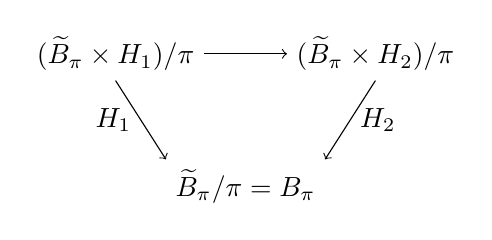
\begin{tikzpicture}[x=1cm,y=1cm]
\node (first) at (-1.65,1.06) {$(\widetilde B_\pi\times H_1)/\pi$};
\node (second) at (1.65,1.06) {$(\widetilde B_\pi\times H_2)/\pi$};
\node (base) at (0,-.62) {$\widetilde B_\pi/\pi=B_\pi$};
\draw[->] (first) -- (second);
\draw[->] (first.south) -- node[left] {$H_1$} (base.north west);
\draw[->] (second.south) -- node[right] {$H_2$} (base.north east);
\end{tikzpicture}}\endgroup}
\end{GelfandAdjacentEvidence}
\begin{GelfandAdjacentEvidence}{GELFAND-P000520}{6}


Но из Кюйпера $(\widetilde B_\pi\times H_i)/\pi\approx B_\pi\times H_i$.
\SourceFigure{GELFAND-P000520}{kuiper-name}{Фамилия в рукописи читается «Кюйпера».}
\end{GelfandAdjacentEvidence}

После отождествл. имеем $B_\pi\times H_1\to B_\pi\times H_2$,
задающее $\varphi_x:H_1\to H_2$.


\Needspace{7\baselineskip}
\begin{GelfandAdjacentEvidence}{GELFAND-P000521}{1}
\SourcePage{GELFAND-P000521}{unlabelled}
\uuline{15/\mbox{$\overline{\underline{X}}$}-73}\qquad \uline{Сем. Гельфанда.}

\uuline{Рудаков.}\qquad
\uwave{О представлениях бесконечномерных алгебр Ли.}

Рассм. $W_n$ — алг. Ли форм. вект. полей
([вписано снизу: непр.] дифф. кольца $k[[x_1,\ldots,x_n]]$).
\SourceFigure{GELFAND-P000521}{continuous-insertion}{Обведённое «непр.» вписано снизу перед «дифф.».}
\end{GelfandAdjacentEvidence}
\begin{GelfandAdjacentEvidence}{GELFAND-P000521}{2}

\[
\left(\sum_{i=1}^{n}a_i(x_1,\ldots,x_n)\frac{\partial}{\partial x_i}\right)
\]
\[
W_n=\mathcal L\supset \text{[зачёркнуто]}\;M\supset M'.
\]
\Unclear{GELFAND-P000521}{upper-chain-cancel}{Под зачёркиванием перед $M$ видны нижние петли. Возможно, это также $M$.}
\end{GelfandAdjacentEvidence}
\begin{GelfandAdjacentEvidence}{GELFAND-P000521}{3}

[под $M$: подалг.]
\Incomplete{GELFAND-P000521}{upper-subalgebra-cancel}{Под «подалг.» зачёркнутые слова не читаются.}
\end{GelfandAdjacentEvidence}
\begin{GelfandAdjacentEvidence}{GELFAND-P000521}{4}

[под $M'$:] идеал конечн. коразм. в $M$.

Пусть дано предст. 
\[
M/M'\longrightarrow\text{предст. }M
\underset{\text{индуц.}}{\longrightarrow}\text{представл. }\mathcal L.
\]

\uline{Теор.}: все неприв. предст. $W_n$ получ. так, кроме конечного числа исключений.

Пр-ва \uwave{счетномерные} дискретные (без топ.). $E$

[под словом «счетномерные»: (вект. пр-ва)]

Предст. $\varrho:\mathcal L\longrightarrow\operatorname{Aut}E$, причём
\[
x\in E,\ \exists V\subset\mathcal L\qquad \varrho(v)x=0.
\qquad\text{(лок. пост. ф-и).}
\]
[под $V$: окр. $0$]
\SourceFigure{GELFAND-P000521}{representation-argument}{В скобках у $\varrho$ написано строчное $v$, а в условии слева прописное $V$.}
\end{GelfandAdjacentEvidence}
\begin{GelfandAdjacentEvidence}{GELFAND-P000521}{5}


Фильтрации окр. нуля
\[
\mathcal L=\mathcal L_{-1}\supset\mathcal L_0\supset\ldots
\supset\mathcal L_k\supset\ldots
\]
\[
\mathcal L_k=\left\{\sum a_i\frac{\partial}{\partial x_i}\
\text{[зачёркнуто]},\ \text{степ. }a_i\geqslant k+1\right\}.
\]
\Incomplete{GELFAND-P000521}{filtration-cancel}{Зачёркнутая запись между производной и запятой не читается.}
\end{GelfandAdjacentEvidence}
\begin{GelfandAdjacentEvidence}{GELFAND-P000521}{6}


\uline{Утвержд.}: рассм. непр. предст. $\mathcal L_0/\mathcal L_k$
и неприв. предст. (и индуцир. представления).

\uwave{Исключения:} в \uline{сопр. пр-вах к} пр-вам замкнутых форм

Пусть есть предст. алг. $\mathcal L$.
\[
x\in E;\quad p(x)=\{\min p:\mathcal L_p x=0\}
\]
($\exists$ ли огр. непр. представл.).

Рассм.
\[
\bar p(E)=\min_{\substack{x\in E,\ x\ne0}}p(x).
\]
\[
E_0=\{x\in E,\ p(x)=\bar p(E)\}\text{ — }\mathcal L_0\text{-подмодуль}.
\]
Если $\bar p(E)>1$, то предст. индуцировано: $E=\operatorname{Ind}(E_0)$
\Unclear{GELFAND-P000521}{induction-bound}{Цифра обведена. Нижний штрих похож на основание $1$, но из-за наложения штрихов чтение условно.}
\end{GelfandAdjacentEvidence}


\begin{center}— · —\end{center}
\uline{Исключения}:
\[
\Omega^p\text{ — форм. формы степ. }p,\qquad
d\Omega^p\text{ — точные формы,}
\]
\[
(d\Omega^p)^*\text{ — сопр. пр-во (с топологией ест.)}
\]
\begin{center}— · —\end{center}
Для гамильтоновых тоже есть соотв. результаты.
\begin{center}— · —\end{center}


\Needspace{7\baselineskip}
\begin{GelfandAdjacentEvidence}{GELFAND-P000522}{1}
\SourcePage{GELFAND-P000522}{23}
\uline{Кириллов.}\qquad \uline{Похожий результ. о группе}

Не доказана, но хорошо известна

$M$ — мн-зие, $\operatorname{Diff}M$ — гр. диффеом.
\Unclear{GELFAND-P000522}{manifold-abbreviation}{Сокращение читается «мн-зие». Вероятно, имеется в виду «многообразие».}
\end{GelfandAdjacentEvidence}
\begin{GelfandAdjacentEvidence}{GELFAND-P000522}{2}


опис. те предст., к-рые имеют конечн. функц. размерность.
\[
\operatorname{Diff}M\supset H_{x_1,\ldots,x_n}
\]
[под $H_{x_1,\ldots,x_n}$:] ост. на месте $x_1,\ldots,x_n$.

Рассм. непр. предст. $H/H_0$ и индуц.

[справа:] $H_0$ сохр. инфин. окр. пор. $n$.

\uuline{Фукс.} (continuation).

$f:C\longrightarrow C'$ функтор

[под $C$, $C'$:] малые кат.
\[
Y\in\operatorname{Ob}C',\qquad Y\backslash f
\]
\[
\operatorname{Ob}(Y\backslash f)=
\{(X,u),\ X\in\operatorname{Ob}C,\ u:Y\longrightarrow f(X)\}.
\]
\[
v:Y\longrightarrow Y'\quad\rightsquigarrow\quad
v\backslash f:Y'\backslash f\longrightarrow Y\backslash f
\]
$\exists$ ест. отобр.
\[
B(Y\backslash f)\longrightarrow
\text{гомот. слой отобр. }Bf:BC\longrightarrow BC'
\]
над точкой $Y\in BC'$.

\[
\longleftarrow\ \cdot\ \longrightarrow
\]
\uuline{новая катег.} пар $(X,u)$, где $X\in\operatorname{Ob}C$,
$u:f(X)\longrightarrow Y$
\SourceFigure{GELFAND-P000522}{dual-comma-box}{%
\begingroup\color{black}\GelfandFitDiagram{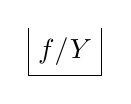
\begin{tikzpicture}
\node (dual) at (0,0) {$f/Y$};
\draw (dual.north west) -- (dual.south west) -- (dual.south east) -- (dual.north east);
\end{tikzpicture}}\endgroup}
\end{GelfandAdjacentEvidence}
\begin{GelfandAdjacentEvidence}{GELFAND-P000522}{3}

другая модель гомот. слоя.

Теор. тоже верна (\uuline{дуальная})

\uline{Теорема A.} Это усл. вып., если все катег. $Y\backslash f$ стягиваемы
(т.е.
\Incomplete{GELFAND-P000522}{theorem-a-cancel}{Слово после «т.е.» зачёркнуто. Чтение не установлено.}
\end{GelfandAdjacentEvidence}
\begin{GelfandAdjacentEvidence}{GELFAND-P000522}{4}

имеют стягиваемые классиф. пр-ва). Тогда вып. и заключение
(в частности, точн. гомот. посл.) $\Rightarrow$
$Bf:BC\longrightarrow BC'$ индуц. изом. гомот. групп.

\begin{center}— · —\end{center}
\uuline{\mbox{$K_i(M)$}}

$M$ — полная подкатег. аб. катег. $A$, замкн. отн. расширений, т.е. из
\[
0\longrightarrow X'\longrightarrow X\longrightarrow X''\longrightarrow0,
\quad X',X''\in\operatorname{Ob}M
\quad\Rightarrow\quad X\in\operatorname{Ob}M.
\]
Если морфизм $i:X'\longrightarrow X$ (из $M$) включ. в короткую точн. посл.,
то он наз. допустимым мономорфизмом.
\SourceFigure{GELFAND-P000522}{exact-sequence-insertion}{%
\begingroup\color{black}\GelfandFitDiagram{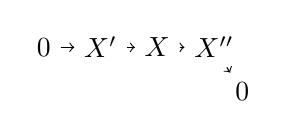
\begin{tikzpicture}[x=.8cm,y=.8cm]
\node (zero) at (0,0) {$0$};
\node (sub) at (.9,0) {$X'$};
\node (middle) at (1.8,0) {$X$};
\node (quotient) at (2.7,0) {$X''$};
\node (end) at (3.15,-.7) {$0$};
\draw[->] (zero) -- (sub);
\draw[->] (sub) -- (middle);
\draw[->] (middle) -- (quotient);
\draw[->] (quotient) -- (end);
\end{tikzpicture}}\endgroup\par\smallskip Последний знак в правой приписке условно прочитан как нуль.}
\end{GelfandAdjacentEvidence}
\begin{GelfandAdjacentEvidence}{GELFAND-P000522}{5}

(точн. поним. в $A$)

Двойств. опр.: если морф. $p:X\longrightarrow X''$ вкл. в кор. точн. посл.,
то назыв. доп. эпиморфизмом.

\SourceFigure{GELFAND-P000522}{pullback-diagram}{%
\begingroup\color{black}\GelfandFitDiagram{\begin{tikzpicture}[x=1cm,y=1cm]
\node (pullback) at (0,1.65) {$Y\times_X Z$};
\node (upper) at (2.1,1.65) {$Y$};
\node (lower) at (0,0) {$Z$};
\node (base) at (2.1,0) {$X$};
\draw[->] (pullback) -- (upper);
\draw[->] (pullback) -- (lower) node[midway,inner sep=0pt] {$\ast$};
\draw[->] (upper) -- node[right] {доп. эпим.} (base);
\draw[->] (lower) -- node[above] {произв.} node[below] {морф.} (base);
\node[anchor=west] at (4.1,0) {$(M)$};
\end{tikzpicture}}\endgroup}
\end{GelfandAdjacentEvidence}


Тогда $Y\times_X Z\in\operatorname{Ob}M$
и $\mathord{\ooalign{\hfil$\downarrow$\hfil\cr\hfil$\scriptstyle\ast$\hfil\cr}}$
— доп. эпим..


\Needspace{7\baselineskip}
\begin{GelfandAdjacentEvidence}{GELFAND-P000523}{1}
\SourcePage{GELFAND-P000523}{unlabelled}
По $M$ строим катег. $QM$:
\[
\operatorname{Ob}M=\operatorname{Ob}QM.
\]
\[
\operatorname{Mor}_{QM}(X_1,X_2)=
\left\{X_1\overset{\text{д.э.}}{\longleftarrow}X
\overset{\text{д.м.}}{\longrightarrow}X_2\right\}.
\]
Опр. эквив. очев. образом.

([зачёркнуто] $X_1$ — допуст. подфактор $X_2$)
\Incomplete{GELFAND-P000523}{subquotient-cancel}{Зачёркнутая запись перед $X_1$ не читается.}
\end{GelfandAdjacentEvidence}
\begin{GelfandAdjacentEvidence}{GELFAND-P000523}{2}


\uwave{Опр. композиции:}
\SourceFigure{GELFAND-P000523}{composition-corrections}{%
\begingroup\color{black}\GelfandFitDiagram{\begin{tikzpicture}[x=1.3cm,y=1cm,every node/.style={inner sep=2pt}]
\node (one) at (0,0) {$X_1$};
\node (left) at (1,0) {$X$};
\node (two) at (2,0) {$X_2$};
\node (right) at (3,0) {$X'$};
\node (three) at (4,0) {$X_3$};
\node (pb) at (2,-1.04) {$X_4$};
\draw[->] (left) -- node[above] {\scriptsize д.э.} (one);
\draw[->] (left) -- node[above] {\scriptsize д.м.} (two);
\draw[->] (right) -- node[above] {\scriptsize д.э.} (two);
\draw[->] (right) -- node[above] {\scriptsize д.м.} (three);
\draw[->] (pb) -- node[below left] {\scriptsize д.э.} (left);
\draw[->] (pb) -- node[below right] {\scriptsize д.м.} (right);
\end{tikzpicture}}\endgroup\par\smallskip
$X_4=X\underset{X_2}{\times}X'$.\par\smallskip В нижней вершине и в формуле произведения индекс $4$ написан поверх прежнего знака. Прежний знак не читается. У нижнего конца левой наклонной стрелки виден короткий штрих.}
\end{GelfandAdjacentEvidence}
\begin{GelfandAdjacentEvidence}{GELFAND-P000523}{3}


и надо взять
\[
X_1\overset{\text{д.э.}}{\longleftarrow}X_4
\overset{\text{д.м.}}{\longrightarrow}X_3.
\]
По определению
\[
K_i(M)=\pi_{i+1}(BQM,0),
\]
где $0$ — произвольный из 0-х объектов категории $M$.

Классы изом. объектов $M$ должны образ. множество.

\Incomplete{GELFAND-P000523}{particular-case-cancel}{Зачёркнутая запись перед «Частный случай» не читается.}
\end{GelfandAdjacentEvidence}
\begin{GelfandAdjacentEvidence}{GELFAND-P000523}{4}

\uline{Частный случай:} (основной).

$A$ — произв. кольцо, $PA$ — кат. кон.-порожд. левых проект. $A$-модулей.
\SourceFigure{GELFAND-P000523}{definition-bracket}{%
\begingroup\color{black}\GelfandFitDiagram{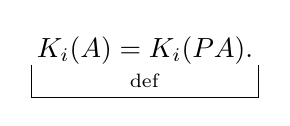
\begin{tikzpicture}
\node (definition) {$K_i(A)=K_i(PA)$.};
\node[font=\scriptsize] at (0,-.38) {$\mathrm{def}$};
\draw (-1.44,-.18) -- (-1.44,-.59) -- (1.44,-.59) -- (1.44,-.18);
\end{tikzpicture}}\endgroup}
\end{GelfandAdjacentEvidence}
\begin{GelfandAdjacentEvidence}{GELFAND-P000523}{5}


\sout{Св-ва некотор. \mbox{$K$}-функтора.}
\Unclear{GELFAND-P000523}{cancelled-k-heading}{Зачёркнутое сокращение между «Св-ва» и буквой K условно прочитано «некотор.».}
\end{GelfandAdjacentEvidence}
\begin{GelfandAdjacentEvidence}{GELFAND-P000523}{6}


\[
\underset{\longrightarrow}{\lim}\operatorname{GL}(n,A)=\operatorname{GL}(A).
\]
\[
B\operatorname{GL}(A)
\]
Строим $B_+\operatorname{GL}(A)$ со св-вами

1) оно $H$-пр-во,

2) $B\operatorname{GL}(A)\longrightarrow B_+\operatorname{GL}(A)$

3) гомот. слой ацикличен

4) сурж. отобр. $\pi_1$.

\[
K_i(A)=\pi_{i+1}(B_+\operatorname{GL}(A))
\text{ — старое опред. (Квиллена)}
\]
\SourceFigure{GELFAND-P000523}{old-index-as-written}{Индекс $i+1$ в этой формуле набран по рукописи.}
\end{GelfandAdjacentEvidence}
\begin{GelfandAdjacentEvidence}{GELFAND-P000523}{7}


\Unclear{GELFAND-P000523}{apparent-cancel}{Перед «По-видимому» зачёркнута запись, возможно начатое «По».}
\end{GelfandAdjacentEvidence}
\begin{GelfandAdjacentEvidence}{GELFAND-P000523}{8}

По-видимому $BQPA$ это $B_+\operatorname{GL}(A)$. Это не так, но есть отобр.
\[
B\operatorname{GL}(A)\longrightarrow BQPA.
\]
Пусть $S_n$ — своб. $A$-мод. с $n$ образ..
\[
S_n\in\operatorname{Ob}(PA)=\operatorname{Ob}(QPA).
\]
Элем. группы $\operatorname{GL}(n,A)$ — это автом. $S_n\longrightarrow S_n$.
Это позв. опр. функтор
\[
\operatorname{GL}(n,A)\rightsquigarrow PA.
\]
[под $\operatorname{GL}(n,A)$:] соотв. кат. (единст. об.)
\[
\text{об.}\longrightarrow S_n
\]
\SourceFigure{GELFAND-P000523}{pa-vertical-note}{$\Vert$\quad автом. в $PA$ явл. морф. в $QPA$}
\end{GelfandAdjacentEvidence}


Функтор $\operatorname{GL}(n,A)\longrightarrow QPA$.


\Needspace{7\baselineskip}
\begin{GelfandAdjacentEvidence}{GELFAND-P000524}{1}
\SourcePage{GELFAND-P000524}{24}
Отсюда получ. отобр. классиф. пр-в
\[
B\operatorname{GL}(n,A)\longrightarrow BQPA
\]
Остаётся пред. переход. (они не согласованы).
\[
\begin{aligned}
QPA&\longrightarrow QPA\\
X&\longrightarrow X\oplus A
\end{aligned}
\qquad\text{явл. гомотопич. эквивал.}
\]
Диагр.
\SourceFigure{GELFAND-P000524}{stabilization-square}{%
\begingroup\color{black}\GelfandFitDiagram{\begin{tikzpicture}[x=1cm,y=1cm]
\node (a) at (0,1.22) {$B\operatorname{GL}(n,A)$};
\node (b) at (2.9,1.22) {$BQPA$};
\node (c) at (0,0) {$B\operatorname{GL}(n+1,A)$};
\node (d) at (2.9,0) {$BQPA$};
\draw[->] (a) -- (b);
\draw[->] (c) -- (d);
\draw[->] (a) -- (c);
\draw[->] (b) -- (d);
\node (commutes) at (4.62,.63) {\small коммут.};
\draw[<-] (commutes.south west) -- (commutes.south east);
\end{tikzpicture}}\endgroup}
\end{GelfandAdjacentEvidence}

и отсюда предел и отобр.
\[
B\operatorname{GL}(A)\longrightarrow BQPA
\]


\Needspace{7\baselineskip}
\begin{GelfandAdjacentEvidence}{GELFAND-P000525}{1}
\SourcePage{GELFAND-P000525}{unlabelled}
\uline{22.10.73}\qquad\uline{Сем. Гельфанда.}

\Incomplete{GELFAND-P000525}{speaker-cancellation}{Зачёркнутая запись перед «Гельфанд» не читается.}
\end{GelfandAdjacentEvidence}
\begin{GelfandAdjacentEvidence}{GELFAND-P000525}{2}

\uline{Гельфанд.} \uwave{Реклама раб. по нелин. теории рассеяния.} (Straus)
\SourceFigure{GELFAND-P000525}{straus-spelling}{Фамилия в скобках написана «Straus».}
\end{GelfandAdjacentEvidence}
\begin{GelfandAdjacentEvidence}{GELFAND-P000525}{3}

\[
U(t)U(s)=U(t+s),
\]
Связь $U(t)f$ при $t\longrightarrow\pm\infty$

Типичные черты: $E(U(t)f)=E(f)$; $E$ — нек-рый ф-л

$\exists$ более прост. группа $U_0(t)$, такая что
\[
E\bigl(U(t)f-U_0(t)f_{\pm}\bigr)\underset{t\to\pm\infty}{\longrightarrow}0
\qquad(\exists f_{\pm})
\]
$S$ — связь $f_+$ и $f_-$.

Примеры: волн. ур-е
\[
u_{tt}-\Delta u+u+|u|^2u=0;
\]
\Unclear{GELFAND-P000525}{wave-sign}{Знак перед лапласианом обведён. По горизонтальному штриху условно прочитан минус.}
\end{GelfandAdjacentEvidence}
\begin{GelfandAdjacentEvidence}{GELFAND-P000525}{4}

\SourceFigure{GELFAND-P000525}{kdv-time-index}{%
\begingroup\color{black}\GelfandFitDiagram{\begin{tikzpicture}[x=1cm,y=1cm]
\node (equation) at (0,0) {$u_\tau+u_{xxx}+uu_x=0$};
\node (label) at (3.25,.85) {\small ур-е де Фриса};
\draw[->] (label.south west) to[out=205,in=5] (equation.east);
\end{tikzpicture}}\endgroup\par\smallskip Первый нижний индекс условно набран как $\tau$ по форме штриха. Он отличается от $tt$ в строке выше.}
\end{GelfandAdjacentEvidence}
\begin{GelfandAdjacentEvidence}{GELFAND-P000525}{5}

\begin{center}— $\bullet$ —\end{center}

\uline{Кириллов.}

1. \uwave{Раб. Костанта.}

$M$ — симплектич. мн-зие (зад. невыр. замкн. 2-форма $\omega$).

$TM$ — рассл. над $M$ со структ. гр. $\operatorname{Sp}(2n,\mathbb R)$. Она неодносвязна.

Топологич.
\SourceFigure{GELFAND-P000525}{covering-diagram}{%
\begingroup\color{black}\GelfandFitDiagram{\begin{tikzpicture}[x=1cm,y=1cm]
\node (sp) at (0,1.05) {$\operatorname{Sp}(2n,\mathbb R)$};
\node[anchor=west] at (sp.east) {$\approx U(n)$};
\node (cover) at (0,0) {$M(2n,\mathbb R)$};
\node[anchor=west] at (1.7,0) {\small (2-листное накр.)};
\draw[->] (cover) -- (sp);
\end{tikzpicture}}\endgroup}
\end{GelfandAdjacentEvidence}
\begin{GelfandAdjacentEvidence}{GELFAND-P000525}{6}

Иногда структ. гр. поднимается до
\Incomplete{GELFAND-P000525}{covering-cancellation}{Зачёркнутый знак перед $M(2n,\mathbb R)$ не читается.}
\end{GelfandAdjacentEvidence}
\begin{GelfandAdjacentEvidence}{GELFAND-P000525}{7}

$M(2n,\mathbb R)$.

Тогда на $M$ строится спинорное расслоение (если $C_1$ делится на 2).

$M$ имеет спец.
\Incomplete{GELFAND-P000525}{representation-cancellation}{Зачёркнутое слово перед «предст. $T$» не читается.}
\end{GelfandAdjacentEvidence}
\begin{GelfandAdjacentEvidence}{GELFAND-P000525}{8}

предст. $T$, наз. спинорным (или же предст. Вейля)

Ал. $\{p_1,\ldots,p_n,q_1,\ldots,q_n\}$ и соотн.
\[
p_iq_j-q_jp_i=\delta_{ij}
\]
\SourceFigure{GELFAND-P000525}{algebra-abbreviation}{В начале строки читается сокращение «Ал.».}
\end{GelfandAdjacentEvidence}

(если $+$, то спин. предст. ортог. группы).

$\operatorname{Sp}(2n,\mathbb R)$ лин. меняет $p$ и $q$.

Реализ.
$p_i\longrightarrow\frac{\partial}{\partial x_i}$,
$q_i\longrightarrow x_i$ в $L^2(\mathbb R^n)$.

Автом. алг. $\Longrightarrow$ автом. алг. огр. операторов.
Но все они внутренние: $A\longrightarrow UAU^{-1}$
($U$ с точн. до множ.) $\Rightarrow$ проективное представление.
Множители сводятся к $\pm1$.
Предст. делается однозн. на 2-листном накрытии.


\Needspace{7\baselineskip}
\begin{GelfandAdjacentEvidence}{GELFAND-P000526}{1}
\SourcePage{GELFAND-P000526}{28}
2. \uwave{[зачёркнуто] \mbox{$p$}-адич. меры}.
\Incomplete{GELFAND-P000526}{title-cancellation}{Зачёркнутый фрагмент заголовка не прочитан.}
\end{GelfandAdjacentEvidence}
\begin{GelfandAdjacentEvidence}{GELFAND-P000526}{2}


$p$-адич. меры; $\mathbb Z_p$ — целые;
\Incomplete{GELFAND-P000526}{integers-cancellation}{Зачёркнутая запись после «целые» не читается.}
\end{GelfandAdjacentEvidence}
\begin{GelfandAdjacentEvidence}{GELFAND-P000526}{3}


Рассм. $C(\mathbb Z_p,K)$, $K$ — расш. $p$-адич. поля (конечное)

(непр. ф-и со зн. в $K$)
\[
\operatorname{Hom}\bigl(C(\mathbb Z_p,K),\mathbb Q_p\bigr)
=C(\mathbb Z_p,K)'=M(\mathbb Z_p,K)
\]
(меры с $p$-адич. знач.)
\SourceFigure{GELFAND-P000526}{dual-codomain}{Второй аргумент $\operatorname{Hom}$ читается как $\mathbb Q_p$.}
\end{GelfandAdjacentEvidence}
\begin{GelfandAdjacentEvidence}{GELFAND-P000526}{4}


На мерах есть свёртка
\SourceFigure{GELFAND-P000526}{convolution-bracket}{%
\begingroup\color{black}\GelfandFitDiagram{\begin{tikzpicture}
\node[inner sep=0pt,font=\small] (left) at (0,0) {$\displaystyle\int f\,d(\mu*\nu)=\int$};
\node[inner sep=0pt,font=\small,anchor=west] (inner) at ([xshift=2pt]left.east)
 {$\displaystyle\left(\int f(x+y)\,d\mu(x)\right)$};
\node[inner sep=0pt,font=\small,anchor=west] (right) at ([xshift=2pt]inner.east) {$d\nu(y)$};
\draw (inner.south west) -- ++(0,-.11) -| (inner.south east);
\node[font=\small,anchor=north,yshift=-2mm] at (inner.south) {непр. ф-я};
\end{tikzpicture}}\endgroup}
\end{GelfandAdjacentEvidence}
\begin{GelfandAdjacentEvidence}{GELFAND-P000526}{5}


\uline{Теорема 1.}
\Incomplete{GELFAND-P000526}{theorem-one-cancellation}{Зачёркнутая запись после «Теорема 1» не прочитана.}
\end{GelfandAdjacentEvidence}
\begin{GelfandAdjacentEvidence}{GELFAND-P000526}{6}

$K$-алгебра мер $M(\mathbb Z_p,K)=K[[T]]$.
\[
\left\|\sum a_kT^k\right\|=\sup_k|a_k|
\qquad\text{(ряды с конечн. нормой)}
\]
Форм. ряды получ. из неогр. мер.

\uline{Теорема 2.} Рассм. $M(\mathbb Z_p^*,K)=(p-1)K[[T]]$.

Неогр. меры — конечно-адд. на элем. мн-вах (сопр к лок. пост. ф-ям).

\uuline{Док-во} теор. 1.
\[
\mu\longrightarrow\sum a_kT^k,\qquad
\text{где }a_k=\int_{\mathbb Z_p}\frac{x(x-1)\cdots(x-k+1)}{k!}\,d\mu(x)
\]
\[
\sum a_kT^k=\int_{\mathbb Z_p}(1+T)^x\,d\mu(x).
\]
отсюда след., что свёртка мер $\longrightarrow$ произв. рядов.

\SourceFigure{GELFAND-P000526}{shaded-quadrilateral}{%
\begingroup\color{black}\GelfandFitDiagram{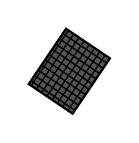
\begin{tikzpicture}[rotate=-34,scale=.73]
\fill[black!67] (0,0) rectangle (.92,1.16);
\foreach \x in {.05,.16,...,.89}
  \draw[line width=.45pt] (\x,0) -- (\x,1.16);
\foreach \y in {.07,.18,...,1.1}
  \draw[line width=.5pt] (0,\y) -- (.92,\y);
\draw[thick] (0,0) rectangle (.92,1.16);
\end{tikzpicture}}\endgroup\par\smallskip Наклонный заштрихованный четырёхугольник между формулами. Назначение неясно.}
\end{GelfandAdjacentEvidence}
\begin{GelfandAdjacentEvidence}{GELFAND-P000526}{7}

\[
1+T=e^\tau\qquad\text{($\tau$ — форм. перем.)}
\qquad\int_{\mathbb Z_p}e^{\tau x}\,d\mu(x)=\widetilde{\mu}(\tau)
\]
(переписать анализ!)

$\tau$ можно счит. числом.
\[
\tau=\ln(1+T)=T-\frac12T^2+\frac13T^3-\ldots
\]
Неясно, какой запас ф-й получится (после замены должен получ. ряд с целыми коэфф.)

\uuline{Пример}
([зачёркнуто])
\uwave{(Картье) в изл. Гельфанда}
\Incomplete{GELFAND-P000526}{example-cancellation}{Фрагмент в первых скобках после «Пример» зачёркнут и не читается.}
\end{GelfandAdjacentEvidence}
\begin{GelfandAdjacentEvidence}{GELFAND-P000526}{8}


Рассм.
\[
\ln(1-a)=a+\frac{a^2}{2}+\frac{a^3}{3}+\ldots
\qquad\text{и }a=2\in\mathbb Z_2.
\]
\SourceFigure{GELFAND-P000526}{logarithm-signs}{После знака равенства в рукописи стоит $a$, затем знаки плюс.}
\end{GelfandAdjacentEvidence}
\begin{GelfandAdjacentEvidence}{GELFAND-P000526}{9}

Ряд сходится [вписано снизу: и равен] $\ln(-1)$.
\SourceFigure{GELFAND-P000526}{log-equality-insertion}{Обведённая вставка «и равен» направлена к строке выше.}
\end{GelfandAdjacentEvidence}
\begin{GelfandAdjacentEvidence}{GELFAND-P000526}{10}

\[
\ln[(-1)^2]=2\ln(-1)=0\quad\Rightarrow\quad\ln(-1)=0.
\]
отсюда ряд сходится к 0
\[
2+\frac{2^2}{2}+\frac{2^3}{3}+\frac{2^4}{4}+\frac{2^5}{5}
+\ldots+\frac{2^n}{n}+\ldots=0
\]
\[
S_n=2+\frac{2^2}{2}+\frac{2^3}{3}+\ldots+\frac{2^n}{n}
\qquad\text{при большом $n$ делится на }2^k
\]
$2$, $4$, $\dfrac{20}{3}$, $\dfrac{32}{3}$ и т. д.
\begin{center}— $\cdot$ —\end{center}

\uline{Теорема.}
\[
\|\mu\|=\sup_k|a_k|\qquad(\approx\text{ Планшереля})
\]
\[
\|\mu\|\underset{\mathrm{def}}{=}\sup_{|f|\leq1}\left|\int f\,d\mu\right|
\]
Из ф-лы $\|\mu\|\geq\sup_k|a_k|$

Надо пров.
\[
\begin{gathered}
|f|\leq1\quad\Rightarrow\quad f(x)=\sum c_kP_k(x),\qquad |c_k|\leq1,\\
P_k(x)=\frac{x(x-1)\cdots(x-k+1)}{k!}
\end{gathered}
\]
(\uline{Док-во}: приблиз. многочленами и применяем теор.)
\[
c_k=\sum_{i=0}^k(-1)^{i+k}C_k^if(i)=\Delta^kf(0)
\qquad\text{(ф-ла Тейлора)}
\]
\[
\begin{aligned}
X^{\tikz[baseline=(degree.base)]{\node[draw,circle,inner sep=.4pt] (degree) {$\scriptstyle k$};}}
&=x(x-1)\cdots(x-k+1),\\
\Delta X^{\tikz[baseline=(degree.base)]{\node[draw,circle,inner sep=.4pt] (degree) {$\scriptstyle k$};}}
&=kx^{\tikz[baseline=(degree.base)]{\node[inner sep=.5pt] (degree) {$\scriptstyle k-1$};
 \draw (degree.center) ellipse (.22 and .11);}},
\qquad\text{где }\Delta f(x)=f(x+1)-f(x).
\end{aligned}
\]
\Unclear{GELFAND-P000526}{falling-variable}{Первые две буквы с обведённым индексом условно набраны как $X$, а буква после множителя $k$ — как $x$.}
\end{GelfandAdjacentEvidence}



\Needspace{7\baselineskip}
\begin{GelfandAdjacentEvidence}{GELFAND-P000527}{1}
\SourcePage{GELFAND-P000527}{unlabelled}
\[
f(x)=\sum_{k=0}^{\infty}\frac{1}{k!}
X^{\tikz[baseline=(degree.base)]{\node[draw,circle,inner sep=.4pt] (degree) {$\scriptstyle k$};}}
\cdot f^{\tikz[baseline=(degree.base)]{\node[inner sep=.4pt] (degree) {$\scriptstyle(k)$};
  \draw (degree.center) ellipse (.20 and .13);}}(0),
\qquad
\text{где } f^{\tikz[baseline=(degree.base)]{\node[inner sep=.4pt] (degree) {$\scriptstyle(k)$};
  \draw (degree.center) ellipse (.20 and .13);}}(x)=(\Delta^k f)(x)
\]
\SourceFigure{GELFAND-P000527}{series-notation}{В первом произведении буква с обведённым $k$ читается как $X$. Оба показателя $(k)$ у $f$ тоже обведены.}
\end{GelfandAdjacentEvidence}
\begin{GelfandAdjacentEvidence}{GELFAND-P000527}{2}


\uline{Утв.}: $\forall$ непр. ф-и
\Incomplete{GELFAND-P000527}{top-cancellation}{Слово перед «ряд» зачёркнуто и не читается.}
\end{GelfandAdjacentEvidence}
\begin{GelfandAdjacentEvidence}{GELFAND-P000527}{3}

ряд Маклорена равном. сходится, причём,
\[
\max|f|=\max|a_k|.
\]
\Unclear{GELFAND-P000527}{modulus-stroke}{Перед $f$ в рукописи толстый штрих. Он условно набран как одна черта модуля.}
\end{GelfandAdjacentEvidence}
\begin{GelfandAdjacentEvidence}{GELFAND-P000527}{4}


\uwave{След. раз Кириллов (ещё 3 мин.) и Мищенко.}

\uuline{Фукс}. (продолжение).

$M$ — адд. полн. подкат. аб., замкн. отн. расширений
\[
QM:\qquad \operatorname{Ob}QM=\operatorname{Ob}M.
\]
\SourceFigure{GELFAND-P000527}{qm-span}{%
\begingroup\color{black}\GelfandFitDiagram{\begin{tikzpicture}[x=1cm,y=1cm]
\node (left) at (0,0) {$X$};
\node (middle) at (2,0) {$X''$};
\node (right) at (4,0) {$X'$};
\draw[->] (middle) -- node[below] {\small доп. э.} (left);
\draw[->] (middle) -- node[below] {\small доп. м.} (right);
\end{tikzpicture}}\endgroup}
\end{GelfandAdjacentEvidence}
\begin{GelfandAdjacentEvidence}{GELFAND-P000527}{5}

\[
\pi_i(BQM)
\]
$BQM$ гомол. эквив. $B\operatorname{GL}(\infty,A)$

\uline{Опред.} \uline{гр. Гротендика категории \mbox{$M$}.}
\uline{Образ.} — \uwave{объекты \mbox{$M$}}, соотнош.
\[
0\to X'\to X\to X''\to0,\qquad\Rightarrow\quad X=X'+X''
\]
Гр. коммут., т.к. $\exists\ X=X'\oplus X''$.

\uuline{Теорема:}
\[
\underset{\substack{\Vert\\\pi_1(BQM,0)}}{K_0(M)}\cong
\text{гр. Гротендика кат. }M.
\]
Нульмерн. остов $=\operatorname{Ob}(M)$

1-мерн. остов — морфизмы $QM$

$\forall X$ опр. петля
\SourceFigure{GELFAND-P000527}{loop-figure}{%
\begingroup\color{black}\GelfandFitDiagram{\begin{tikzpicture}[x=1cm,y=1cm]
\node (zero) at (0,0) {$0$};
\node (x) at (2.15,.83) {$X$};
\draw[->] (zero) to[bend left=30] node[above left] {\small доп. м.} (x);
\draw[->] (x) to[bend left=32] node[below right] {\small $($доп. эп.$)^{-1}$} (zero);
\node at (3.9,.15) {$\zeta_X$.};
\end{tikzpicture}}\endgroup}
\end{GelfandAdjacentEvidence}
\begin{GelfandAdjacentEvidence}{GELFAND-P000527}{6}


Если в $M$ есть точн. посл. (кор.) $0\to X'\to X\to X''\to0$,
то
\[
\zeta_X\sim\zeta_{X'}\cdot\zeta_{X''}.
\]
\Unclear{GELFAND-P000527}{loop-notation}{Буква в обозначении петли условно набрана как $\zeta$.}
\end{GelfandAdjacentEvidence}
\begin{GelfandAdjacentEvidence}{GELFAND-P000527}{7}


\SourceFigure{GELFAND-P000527}{lower-diagram}{%
\begingroup\color{black}\GelfandFitDiagram{\begin{tikzpicture}[x=1cm,y=1cm,every node/.style={inner sep=1.6pt}]
\node (left) at (0,2.38) {$X'$};
\node (middle) at (2.45,2.52) {$X$};
\node (right) at (4.97,2.6) {$X''$};
\node at (2.54,-.04) {$0$};
\draw[->] (left) -- node[above] {\small д.м.} (middle);
\draw[->] (right) -- node[above] {\small д.э.$^{-1}$} (middle);
\draw[black!60,thin] (.24,2.1) -- (1.1,2.53);
\draw[black!60,thin] (.36,1.85) -- (1.66,2.46);
\draw[black!60,thin] (.46,1.63) -- (2.03,2.45);
\draw[black!60,thin] (.76,1.28) -- (2.23,2.02);
\draw[black!60,thin] (1.05,.89) -- (2.08,1.38);
\draw[black!60,thin] (1.23,.59) -- (2.22,1.04);
\draw[black!60,thin] (1.34,.43) -- (2.4,.65);
\draw[black!60,thin] (1.46,.27) -- (2.5,.5);
\draw[->] (1.42,.18) to[out=160,in=265]
  node[pos=.48,left] {\small д.м.} (.46,1.73);
\draw[->] (1.47,.37) to[out=135,in=300]
  node[pos=.64,right] {\small д.э.$^{-1}$} (.71,1.94);
\draw[->] (2.49,.36) to[out=124,in=221]
  node[pos=.45,left] {\small д.м.} (2.39,1.91);
\draw[->] (2.64,.56) to[out=51,in=300]
  node[pos=.65,right] {\small д.э.$^{-1}$} (2.62,1.93);
\draw[->] (3.43,.51) to[out=50,in=194]
  node[pos=.63,above left] {\small д.м.} (4.54,1.5);
\draw[->] (3.53,.28) to[out=18,in=227]
  node[pos=.57,below right] {\small $($д.э.$)^{-1}$} (4.68,1.26);
\end{tikzpicture}}\endgroup\par\smallskip Нижние концы дуг оставлены раздельными, как на рисунке. Тонкими линиями показана наклонная штриховка.}
\end{GelfandAdjacentEvidence}

и вспоминаем про 2-симплексы.

\begin{center}— $\bullet$ —\end{center}


\Needspace{7\baselineskip}
\begin{GelfandAdjacentEvidence}{GELFAND-P000528}{1}
\SourcePage{GELFAND-P000528}{unlabelled}
\uline{29/\mbox{$\overline{\underline{X}}$}-73г.}\qquad\uline{Сем. Гельфанда.}

\uuline{А.А. Кириллов.}

Есть симплектическое мн-зие $M$
\SourceFigure{GELFAND-P000528}{upper-sketch}{%
\begingroup\color{black}\GelfandFitDiagram{\begin{tikzpicture}[x=1cm,y=1cm]
\draw (.94,1.64) .. controls (1.74,1.89) and (2.05,1.57) .. (2.64,1.52)
  .. controls (3.17,1.46) and (3.64,1.25) .. (3.67,.78)
  .. controls (3.78,.28) and (3.05,.02) .. (2.46,.13)
  .. controls (1.99,.28) and (1.58,.12) .. (1.13,.12)
  .. controls (.58,.12) and (.02,.34) .. (.08,.73);
\draw[densely dotted] (.08,.73) .. controls (.10,1.20) and (.44,1.53) .. (.94,1.64);
\draw[rotate around={25:(1.13,.91)}] (1.13,.91) ellipse (.33 and .25);
\draw[rotate around={17:(1.65,1.00)}] (1.65,1.00) ellipse (.42 and .32);
\draw[rotate around={18:(2.16,.96)}] (2.16,.96) ellipse (.33 and .25);
\draw (1.97,1.19) .. controls (2.07,1.28) and (2.20,1.32) .. (2.29,1.29);
\end{tikzpicture}}\endgroup}
\end{GelfandAdjacentEvidence}
\begin{GelfandAdjacentEvidence}{GELFAND-P000528}{2}


\SourceFigure{GELFAND-P000528}{covering-map}{%
\begingroup\color{black}\GelfandFitDiagram{\begin{tikzpicture}
\node (sp) at (0,1.0) {$\operatorname{Sp}(2n,\mathbb R)$};
\node (cover) at (0,0) {$M(n,\mathbb R)$};
\node[anchor=west] at (1.47,0) {\small (2-листное накр.)};
\draw[->] (cover) -- (sp);
\end{tikzpicture}}\endgroup}
\end{GelfandAdjacentEvidence}
\begin{GelfandAdjacentEvidence}{GELFAND-P000528}{3}

лок. можно считать
\[
\omega=\sum_{k=1}^n dp_k\wedge dq_k
\]
Ф-и перехода (в $TM$) $g_{ij}\in\operatorname{Sp}(2n,\mathbb R)$

Пусть они в 2-листном накрытии $M(2n,\mathbb R)$
\SourceFigure{GELFAND-P000528}{covering-notation}{В строке написано $M(2n,\mathbb R)$. В схеме выше и во вставке ниже написано $M(n,\mathbb R)$.}
\end{GelfandAdjacentEvidence}
\begin{GelfandAdjacentEvidence}{GELFAND-P000528}{4}


\textbf{Спинорное представление} [вписано снизу: $M(n,\mathbb R)$] в гильб. пр-ве
\Incomplete{GELFAND-P000528}{spinor-cancellation}{Зачёркнутый знак после «пр-ве» не читается.}
\end{GelfandAdjacentEvidence}
\begin{GelfandAdjacentEvidence}{GELFAND-P000528}{5}

индуц. гильбертово расслоение $HM$ над $M$
\SourceFigure{GELFAND-P000528}{spinor-insertion}{Обведённая вставка $M(n,\mathbb R)$ примыкает к слову «представление».}
\end{GelfandAdjacentEvidence}
\begin{GelfandAdjacentEvidence}{GELFAND-P000528}{6}

\[
SM\subset HM\subset S'M
\]
\Unclear{GELFAND-P000528}{schwartz-cancellation}{Зачёркнутый знак перед $S'M$ похож на $H$.}
\end{GelfandAdjacentEvidence}
\begin{GelfandAdjacentEvidence}{GELFAND-P000528}{7}

[под $SM$: быстро убыв.]

Симплектич. преобр. $\leadsto$ опер. в гильб. пр-ве (кан. преобр. с $p_i,q_i$)

Получ. проективное представление
\[
\underbrace{GM}=TM\oplus\mathbb R\times M
\]
[под скобкой:] полин. $\leq2$-й степ. от $p$ и $q$ (Гейзенбергова алг. Ли)
\SourceFigure{GELFAND-P000528}{polynomial-degree}{Перед цифрой $2$ виден знак $\leq$.}
\end{GelfandAdjacentEvidence}
\begin{GelfandAdjacentEvidence}{GELFAND-P000528}{8}


$GM$ действ. на $HM$ соглас. со структур. расслоения.

$RM$, $R_x$ — лагранжевы подпр-ва в $T_xM$ (max разм.)

\uline{А. Шнирельман.}\qquad\uline{О Ферми:} равнораспред. энергии по степ. своб..
\[
\ddot x_k=(x_{k-1}+x_{k+1}-2x_k)+\varepsilon(x_{k-1}-x_k)^2
 +\varepsilon(x_{k+1}-x_k)^2
\]
\SourceFigure{GELFAND-P000528}{dynamics-equation}{В рукописи оба квадратичных члена стоят со знаком плюс.}
\end{GelfandAdjacentEvidence}
\begin{GelfandAdjacentEvidence}{GELFAND-P000528}{9}


\uwave{Реш. числ. на машине}

\underline{$k=16$}\qquad через кон. \sout{времени} промеж. времени смотрели преобр. Фурье.
\Unclear{GELFAND-P000528}{chain-size}{Число $16$ читается. Обведённая буква условно набрана как $k$.}
\end{GelfandAdjacentEvidence}
\begin{GelfandAdjacentEvidence}{GELFAND-P000528}{10}

\Unclear{GELFAND-P000528}{time-cancellation}{Зачёркнутое слово условно прочитано «времени».}
\end{GelfandAdjacentEvidence}
\begin{GelfandAdjacentEvidence}{GELFAND-P000528}{11}

Нач. усл. — \uuline{\mbox{$\sin$}}\qquad (эн. вся в 1-й гарм.)

По оценке $t=10^{-35}$ в этом сост.
\SourceFigure{GELFAND-P000528}{time-exponent}{Показатель степени в строке читается как $-35$.}
\end{GelfandAdjacentEvidence}
\begin{GelfandAdjacentEvidence}{GELFAND-P000528}{12}


\uline{Вычисления:}
\SourceFigure{GELFAND-P000528}{recurrence-plot}{%
\begingroup\color{black}\GelfandFitDiagram{\begin{tikzpicture}[x=.83cm,y=1.05cm,every node/.style={inner sep=1.3pt}]
\draw (-.42,-.02) .. controls (1.6,.13) and (2.7,.06) .. (3.22,.02)
  .. controls (4.6,-.04) and (5.64,-.12) .. (6.36,-.07);
\draw (0,-.39) -- (.04,1.69);
\draw (3.14,-.30) .. controls (3.28,.52) and (3.03,1.01) .. (3.24,1.90);
\draw (6.36,-.05) .. controls (6.30,.56) and (6.52,1.17) .. (6.57,1.92);
\draw[densely dashed,thin] (.04,1.73) .. controls (1.5,1.63) and (2.1,1.79) .. (3.3,1.89);
\draw[densely dashed,thin] (3.67,1.84) -- (6.55,1.85);
\draw[thick] (.04,1.67) .. controls (.56,1.64) and (.90,1.28) .. (1.16,.95)
  .. controls (1.68,.16) and (2.29,.58) .. (2.77,1.27)
  .. controls (2.98,1.59) and (3.13,1.73) .. (3.23,1.72)
  .. controls (3.79,1.68) and (3.92,.33) .. (4.52,.30)
  .. controls (5.30,.14) and (5.28,1.06) .. (6.45,1.35);
\draw (.04,.04) .. controls (.54,.33) and (.56,1.02) .. (1.36,1.16)
  .. controls (1.53,1.20) and (1.41,.65) .. (1.75,.51)
  .. controls (2.15,.15) and (2.08,1.43) .. (2.47,.97)
  .. controls (2.76,.63) and (3.09,.13) .. (3.30,.02);
\draw (.04,.04) .. controls (.83,.21) and (.84,.80) .. (1.50,.93)
  .. controls (1.88,1.04) and (1.76,1.55) .. (2.29,.98)
  .. controls (2.65,.59) and (2.49,.23) .. (3.30,.02);
\draw (.04,.04) .. controls (.48,.13) and (.97,.30) .. (1.20,.52);
\fill (.04,1.67) circle (1.7pt);
\fill (3.23,1.72) circle (1.7pt);
\draw[fill=white,thick] (6.45,1.35) circle (1.7pt);
\node[above right] at (.15,1.69) {\scriptsize 1 гарм};
\node at (.22,.49) {\scriptsize $2$};
\node at (.67,.47) {\scriptsize $3$};
\node at (1.12,.47) {\scriptsize $4$};
\draw[<-] (.09,-.21) -- (1.29,-.18);
\draw[->] (1.87,-.24) -- (3.02,-.15);
\draw[->] (1.41,-.73) -- (1.63,-.08);
\node[anchor=west] at (1.48,-.79) {\scriptsize $\approx50$ мил. периодов.};
\node at (5.22,1.98) {\scriptsize несколько процентов утекло.};
\end{tikzpicture}}\endgroup\par\smallskip Цифры поставлены возле кривых по их положению в рукописи. Их точная привязка и продолжение короткой восходящей линии среди пересечений не установлены.}
\end{GelfandAdjacentEvidence}


больше невязка

10 шагов — пер. $1/3$

\uwave{Еще 10 шагов — снова}\\
\uwave{то же самое!!}

Кубич. нелин. — тоже считалось. Рез. получ. тот же.


\Needspace{7\baselineskip}
\begin{GelfandAdjacentEvidence}{GELFAND-P000529}{1}
\SourcePage{GELFAND-P000529}{unlabelled}
\uwave{Захаров}: аппрокс. дифф. системой с 1-ми интегралами. (Возможная причина)

Струна с $\sin$ — тоже.

Есть нач. данные, для к-рых происх. равном. распределение.
\[
u_{tt}=u_{xx}\qquad\text{на }S^1\quad\text{все траект. замкнуты}
\]
\[
u_{tt}=u_{xx}+\varepsilon f'(u)
\]
Дрейф 1-го порядка траекторий: тоже периодич. для $u_{tt}=u_{xx}-\varepsilon u^3$.

\SourceFigure{GELFAND-P000529}{lagrangian-bundle}{%
\begingroup\color{black}\GelfandFitDiagram{\begin{tikzpicture}[x=1cm,y=1cm,every node/.style={inner sep=1.5pt}]
\node[anchor=west] at (0,2.13) {Фукс};
\draw (0,1.82) rectangle (1.12,1.94);
\foreach \x in {.02,.12,...,1.02}
  \draw (\x,1.82) -- ({\x+.08},1.94);
\node[anchor=west,align=left,text width=4.7cm] at (1.28,2.1)
  {\small $\Lambda$ — совок. лагр. плоскостей в $\mathbb R^{2n}$};
\node (rm) at (1.4,1.38) {$RM$};
\node (m) at (1.4,.26) {$M$};
\draw[->] (rm) -- (m);
\node[anchor=west,align=left,text width=4.1cm] at (1.96,.89)
  {\small — рассл. лагр. плоск. на симпл. подмн-зии};
\draw (0,.37) -- (1.0,.37) -- (1.0,.02) -- (5.35,.02) -- (5.35,.25) -- (6.05,.25);
\end{tikzpicture}}\endgroup\par\smallskip В слове «на» первый штрих густо обведён. Сокращение читается «подмн-зии».}
\end{GelfandAdjacentEvidence}
\begin{GelfandAdjacentEvidence}{GELFAND-P000529}{2}


Мищенко.\par\nobreak
\begingroup\color{black}\GelfandFitDiagram{\begin{tikzpicture}[x=1cm,y=1cm,baseline]
\draw (0,.06) rectangle (2,.19);
\foreach \x in {.02,.15,...,1.84}
  \draw (\x,.06) -- ({\x+.11},.19);
\end{tikzpicture}}\endgroup
\SourceFigure{GELFAND-P000529}{ring-involution-arrow}{%
\begingroup\color{black}\GelfandFitDiagram{\begin{tikzpicture}
\node at (0,.55) {$\Lambda$};
\node at (.59,.17) {$\Rightarrow$};
\node[anchor=west] at (.8,.55) {— кольцо,};
\node[anchor=west] at (.8,0) {(с инвол.)};
\end{tikzpicture}}\endgroup\par\smallskip Знак внизу справа от $\Lambda$ передан как $\Rightarrow$.}
\end{GelfandAdjacentEvidence}
\begin{GelfandAdjacentEvidence}{GELFAND-P000529}{3}


\SourceFigure{GELFAND-P000529}{quadratic-form-outline}{%
\begingroup\color{black}\GelfandFitDiagram{\begin{tikzpicture}[x=1cm,y=1cm,every node/.style={inner sep=1.2pt}]
\node[anchor=west] at (1.6,2.23) {\small $\lambda=\|\lambda_{ij}\|,\quad \lambda_{ij}\in\Lambda$};
\node[anchor=west] at (.23,1.35) {\small $1)\ \lambda^*=\lambda$};
\node[anchor=west] at (.23,.69)
  {\small $2)\ \exists\mu:\quad\mu\lambda=\left(\begin{smallmatrix}1&&0\\&\ddots&\\0&&1\end{smallmatrix}\right)$};
\node[align=left,anchor=west] at (4.89,1.29) {\small квадр.\\форма\\над $\Lambda$};
\draw (4.63,.32) -- (4.63,2.09) (4.71,.32) -- (4.71,2.09);
\draw (.24,.08) .. controls (-.10,.17) and (-.08,1.41) .. (.25,1.57)
  .. controls (.58,1.82) and (1.44,1.45) .. (1.51,1.87)
  .. controls (1.56,2.12) and (1.53,2.52) .. (1.78,2.52)
  -- (4.58,2.42) .. controls (5.26,2.35) and (6.10,2.53) .. (6.15,1.82)
  .. controls (6.25,1.22) and (6.17,.28) .. (5.76,.21)
  .. controls (4.66,.05) and (.85,-.07) .. (.24,.08);
\end{tikzpicture}}\endgroup\par\smallskip Короткий наклонный след между строками единичной матрицы передан как $\ddots$.}
\end{GelfandAdjacentEvidence}
\begin{GelfandAdjacentEvidence}{GELFAND-P000529}{4}


Фредгольмово предст. — тройка $T=\{T_1,F,T_2\}$;

$T_i$ — предст. $\Lambda$ в $\mathcal L(H)$ (с инволюцией), причём
\begin{align*}
&F\ \text{— фредгольмов оператор}\\
FT_1(x)-T_2(x)F&\quad\in\mathrm{comp}\qquad\forall x\in\Lambda.
\end{align*}
\Incomplete{GELFAND-P000529}{fredholm-cancellation}{После второго $F$, перед $\in$, густо зачёркнут фрагмент в скобках.}
\end{GelfandAdjacentEvidence}
\begin{GelfandAdjacentEvidence}{GELFAND-P000529}{5}


Построим $\lambda\in\mathcal L(H\oplus\cdots\oplus H)$ по квадр. форме.
\SourceFigure{GELFAND-P000529}{direct-sum-identification}{%
\(\rotatebox{-72}{$=$}\,H^n\)\par\smallskip Под прямой суммой два наклонных штриха и $H^n$. Штрихи переданы повёрнутым знаком равенства.}
\end{GelfandAdjacentEvidence}
\begin{GelfandAdjacentEvidence}{GELFAND-P000529}{6}

\[
\lambda_{T_1}=(T_1(\lambda_{ij})),\qquad
\lambda_{T_2}=(T_2(\lambda_{ij}))
\]
[справа:] — обратимы и самосопр.

Они огранич., обратимы, самосопряжены.

\SourceFigure{GELFAND-P000529}{fredholm-square}{%
\begingroup\color{black}\GelfandFitDiagram{\begin{tikzpicture}[x=1cm,y=1cm,every node/.style={inner sep=1.5pt}]
\node (a) at (2.77,1.42) {$H^n$};
\node (b) at (4.47,1.42) {$H^n$};
\node (c) at (2.77,0) {$H^n$};
\node (d) at (4.47,0) {$H^n$};
\draw[->] (a) -- node[above] {\small $\lambda_{T_1}$} (b);
\draw[->] (c) -- node[above] {\small $\lambda_{T_2}$} (d);
\draw[->] (a) -- node[left] (left) {\small $F\otimes id$} (c);
\draw[->] (b) -- node[right] {\small $F\otimes id$} (d);
\node (fred) at (.48,.5) {\small фред.};
\draw[->] (fred.east) -- (left.west);
\node[anchor=west] at (2.04,-.56) {\small коммут. $\mathrm{mod}\ \mathrm{comp}$.};
\end{tikzpicture}}\endgroup}
\end{GelfandAdjacentEvidence}
\begin{GelfandAdjacentEvidence}{GELFAND-P000529}{7}


Пусть так выбр. базисы, что
\[
\lambda_{T_1}=\begin{pmatrix}A&0\\0&-B\end{pmatrix}
\qquad
\lambda_{T_2}=\begin{pmatrix}A'&0\\0&-B'\end{pmatrix}
\]
$A,B$ — обр. и самосопр. и $>0$.
\[
F\otimes id=\begin{pmatrix}F_1&F_2\\F_3&F_3\end{pmatrix}
\]
$F_2,F_3\in\mathrm{comp}$.

$\Rightarrow\quad F_1,F_4$ — фредгольмовы
\SourceFigure{GELFAND-P000529}{lower-matrix-index}{В нижнем правом элементе матрицы написано $F_3$. В последней строке написано $F_4$.}
\end{GelfandAdjacentEvidence}



\Needspace{7\baselineskip}
\begin{GelfandAdjacentEvidence}{GELFAND-P000530}{1}
\SourcePage{GELFAND-P000530}{32}
\uline{Определение.}
$\operatorname{sign}_T\lambda=\operatorname{index}F_1-\operatorname{index}F_4$.
\SourceFigure{GELFAND-P000530}{fredholm-index-difference}{В определении стоит разность индексов $F_1$ и $F_4$.}
\end{GelfandAdjacentEvidence}
\begin{GelfandAdjacentEvidence}{GELFAND-P000530}{2}


Оно не зав. от предст. в виде прям. суммы и от предст. в классе экв. квадр. форм.
\SourceFigure{GELFAND-P000530}{upper-rule-dot-rule}{%
\begingroup\color{black}\GelfandFitDiagram{\begin{tikzpicture}[x=1cm,y=1cm]
\draw (0,0) -- (.92,.02) (1.61,.09) -- (2.74,.09);
\fill (1.27,.07) circle (.6pt);
\end{tikzpicture}}\endgroup}
\end{GelfandAdjacentEvidence}
\begin{GelfandAdjacentEvidence}{GELFAND-P000530}{3}


Пусть $M$ — мн-зие (комп.); $\pi_1(M)=\pi$, $\dim M=4K$; $\Lambda=\mathbb Z[\pi]$.
\Unclear{GELFAND-P000530}{dimension-multiple}{Буква после $4$ условно набрана как $K$. Регистр по почерку не установлен.}
\end{GelfandAdjacentEvidence}
\begin{GelfandAdjacentEvidence}{GELFAND-P000530}{4}


Есть квадр. форма $\sigma(M)$ над $\Lambda$. Формула:
\[
\operatorname{sign}_T(\sigma(M))=
\langle \operatorname{ch}\xi_T\cdot L(M),[M]\rangle
\]
$\xi_T$ — рассл. на $M$

Хирцебрух док. при $(\operatorname{ch}\xi_T=1.)$

Конечномерных предст. недостаточно.
\SourceFigure{GELFAND-P000530}{lower-rule-dot-rule}{%
\begingroup\color{black}\GelfandFitDiagram{\begin{tikzpicture}[x=1cm,y=1cm]
\draw (0,0) -- (1.36,.08) (2.16,.11) -- (3.44,.11);
\fill (1.73,.095) circle (.6pt);
\end{tikzpicture}}\endgroup}
\end{GelfandAdjacentEvidence}
\begin{GelfandAdjacentEvidence}{GELFAND-P000530}{5}


\Unclear{GELFAND-P000530}{lower-right-stroke}{На пустом поле справа короткий одиночный наклонный штрих. Чтение как цифры «1» не установлено.}
\end{GelfandAdjacentEvidence}



\Needspace{7\baselineskip}
\begin{GelfandAdjacentEvidence}{GELFAND-P000531}{1}
\SourcePage{GELFAND-P000531}{37}
\uline{12.11.73.}\qquad\uwave{Сем. Гельфанда.}

\uline{В. Пономарёв.}

Пусть в мн-ве есть 2 операции $\cap$ и $+$ с естеств. св-вами
(ассоц., коммут., $x\cap x=x$, $x+x=x$, $a+(a\cap b)=a$, $a\cap(a+b)=a$)
это \uwave{структура}.

\dashuline{Дистрибут. структура}:
\[
\left.\begin{aligned}
a\cap(b+c)&=(a\cap b)+(a\cap c)\\
a+(b\cap c)&=(a+b)\cap(a+c)
\end{aligned}\right]
\]
[справа:] это только системы подмн-в нек-рого мн-ва.
\SourceFigure{GELFAND-P000531}{distributive-bracket}{Два равенства соединены правой квадратной скобкой с припиской.}
\end{GelfandAdjacentEvidence}
\begin{GelfandAdjacentEvidence}{GELFAND-P000531}{2}


\uuline{пример}: структура подпространств с пересеч. и суммой.

отнош. порядка в структуре: $a\le b\Longleftrightarrow a\cap b=a$
\Unclear{GELFAND-P000531}{order-symbol}{Густо обведённый знак между $a$ и $b$ условно набран как $\le$.}
\end{GelfandAdjacentEvidence}
\begin{GelfandAdjacentEvidence}{GELFAND-P000531}{3}


\uline{Модулярная стр.}:
\[
\forall\,a\subseteq b\ \text{и}\ \forall c\qquad
b\cap(a+c)=a+(b\cap c)\qquad \text{(Дедекинд)}
\]
\SourceFigure{GELFAND-P000531}{modular-formula}{В условии модулярности написано $a\subseteq b$.}
\end{GelfandAdjacentEvidence}
\begin{GelfandAdjacentEvidence}{GELFAND-P000531}{4}


(\sout{\mbox{$\forall$}} дистриб. явл. модул., но не наоборот).
\Unclear{GELFAND-P000531}{distr-cancel}{Густо обведённый знак перед «дистриб.» похож на $\forall$.}
\end{GelfandAdjacentEvidence}
\begin{GelfandAdjacentEvidence}{GELFAND-P000531}{5}


стр. подпр-в явл. модулярной, но не дистрибутивной.

\uwave{стр. подмодулей модуля тоже модулярна.}

\uuline{Вопрос}: есть ли ещё тождества или это всё?
(Гипотеза: $\forall$ модул. стр. — стр. подмод. модуля).

Для структ. подпр-в \uline{есть ещё!!}

\hfill\rule{.9cm}{.35pt}\enspace\(\cdot\)\enspace\rule{1cm}{.35pt}\par

Пусть $e_1,\ldots,e_r$ — буквы.
\SourceFigure{GELFAND-P000531}{first-generator-index}{Нижний индекс в первом списке по форме совпадает с $r$ во втором списке и в обозначении образующих ниже.}
\end{GelfandAdjacentEvidence}
\begin{GelfandAdjacentEvidence}{GELFAND-P000531}{6}

Рассм. натян. на них своб. модулярную структуру (полин. от $e_1,\ldots,e_r$ с соотнош.)

линейно эквив. полиномы $P(e_1,\ldots,e_r)\sim Q(e_1,\ldots,e_r)$, если вып. при подстан. подпр-в.

\hfill\rule{.9cm}{.35pt}\enspace\(\cdot\)\enspace\rule{1.25cm}{.35pt}\par

$V$ — кон.-мерное пр-во над полем $k$.

Представление стр. — отобр. в структуру подпр-в $V$ (к-рая обознач. $PG(V,k)$)
\[
\begin{gathered}
\mathcal L\longrightarrow PG(V,k)\\
a\in\mathcal L\quad\text{\sout{\mbox{$\longrightarrow$}}}\quad a\mapsto s(a)\subset V
\end{gathered}
\qquad
\left.\begin{aligned}
ab&\mapsto s(a)s(b)\\
a+b&\mapsto s(a)+s(b)
\end{aligned}\right\Vert
\]
\SourceFigure{GELFAND-P000531}{representation-map}{Стрелки расположены в два ряда. Двойная вертикальная черта стоит после правого столбца.}
\end{GelfandAdjacentEvidence}
\begin{GelfandAdjacentEvidence}{GELFAND-P000531}{7}

\SourceFigure{GELFAND-P000531}{crossed-map-arrow}{Стрелка после $a\in\mathcal L$ переписана или зачёркнута наклонными петлями.}
\end{GelfandAdjacentEvidence}
\begin{GelfandAdjacentEvidence}{GELFAND-P000531}{8}

\Unclear{GELFAND-P000531}{representation-glyph}{Петлеобразная буква условно набрана как $s$ во всех обозначениях представления.}
\end{GelfandAdjacentEvidence}
\begin{GelfandAdjacentEvidence}{GELFAND-P000531}{9}


\hfill\rule{.9cm}{.35pt}\enspace\(\cdot\)\enspace\rule{1.25cm}{.35pt}\par

$\mathcal D^r$ — своб. модулярная структура с $r$ образ. $e_1,\ldots,e_r$.

Предст. — это $V$ и $s(e_1),\ldots,s(e_r)$ — набор подпр-в $E_1^0,\ldots,E_r^0$,
и обр. такой набор опр. представление.
\Incomplete{GELFAND-P000531}{repr-cancel}{Между «Предст. —» и «это $V$» густо зачёркнут фрагмент.}
\end{GelfandAdjacentEvidence}
\begin{GelfandAdjacentEvidence}{GELFAND-P000531}{10}


\uwave{Задача}: описать все предст. $\mathcal D^r$.

\hfill\rule{1.1cm}{.35pt}\enspace\(\cdot\)\enspace\rule{1.3cm}{.35pt}\par

\sout{Элем. \mbox{$a$} наз. совершенным, если}
\SourceFigure{GELFAND-P000531}{crossed-perfect-definition}{Начало определения перечёркнуто одной линией.}
\end{GelfandAdjacentEvidence}
\begin{GelfandAdjacentEvidence}{GELFAND-P000531}{11}


$s_1,V_1;\quad s_2,V_2$
\[
s_1\oplus s_2\text{ — предст. в }V_1\oplus V_2:\qquad
(s_1\oplus s_2)(a)=s_1(a)\oplus s_2(a)
\]
Разложимое представление опр. естеств..

Элем. $a\in\mathcal L$ (вписано сверху: модул. структ.) наз. \uwave{совершенным}, если $\forall$ предст.
$s$ в кон.-мерн. пр-ве $V$ над $\forall$ полем $k$ подпр-во $s(a)$
можно дополнить подпр-вом $V_2$ и предст. разлагается в прям. сумму [вписано снизу:] с прям. слаг. $V_2$.
\Unclear{GELFAND-P000531}{perfect-ending}{После $V_2$ виден завиток с точкой, примыкающий к выносному штриху верхней строки.}
\end{GelfandAdjacentEvidence}
\begin{GelfandAdjacentEvidence}{GELFAND-P000531}{12}


(Или: при неразл. предст. он перех. в $0$ или $1$).
Если $a\sim b$ (лин.), то соверш. одновременно.

\uline{Пример.} Рассм. своб. мод. структ. с $r$ образ. $e_1,\ldots,e_r$. Рассм. элементы
\[
e_{i_1i_2}=e_{i_1}\ [\text{переписанный знак}]\ \sum_{k\ne i_1,i_2}e_k
\]
\Unclear{GELFAND-P000531}{bottom-product}{Знак между $e_{i_1}$ и суммой густо переписан. Его чтение не установлено.}
\end{GelfandAdjacentEvidence}



\Needspace{7\baselineskip}
\begin{GelfandAdjacentEvidence}{GELFAND-P000532}{1}
\SourcePage{GELFAND-P000532}{unlabelled}
\[
e_{i_1i_2\ldots i_e}=e_{i_1}\sum_{\beta\in\Gamma(\alpha)}e_{k_1\ldots k_{e-1}}
\]
\Unclear{GELFAND-P000532}{recurrence-juxtaposition}{Буква длины по форме похожа на $e$ и условно так набрана. Между $e_{i_1}$ и суммой отдельного знака нет.}
\end{GelfandAdjacentEvidence}
\begin{GelfandAdjacentEvidence}{GELFAND-P000532}{2}

\[
\alpha=(i_1,\ldots,i_e),\qquad \beta=(k_1,\ldots,k_{e-1})
\]
\[
\begin{aligned}
\Gamma(\alpha)&=\{\,k_1\ne i_1,i_2;\quad k_2\ne i_2,i_3,k_1;\quad\ldots\\
&\hphantom{=\{\,}\qquad i_1\ne i_2,\quad i_2\ne i_3,\quad\ldots
\end{aligned}
\]
\SourceFigure{GELFAND-P000532}{gamma-conditions}{Вторая строка с условиями на $i_1,i_2,i_3$ написана с отступом. Правой скобки нет.}
\end{GelfandAdjacentEvidence}
\begin{GelfandAdjacentEvidence}{GELFAND-P000532}{3}


\noindent\makebox[.77\linewidth]{\dotfill}\par

\uline{Трив. соверш. элементы}: \(m_t=\sum_{i\ne t}e_i\) — соверш. элементы.

$m_t$ порожд. булеву алг. с $r$ образующими.

\uline{С. Гельфанд.}

\dashuline{Комплекс Брюа — Титса.}

$G$ — $p$-адич. группа, $K$ — макс. комп. подгруппа.

К Б.-Т. — описание $G/K$, аналог симметрич. пр-ва.
\SourceFigure{GELFAND-P000532}{complex-abbreviation}{Сокращение набрано как «К Б.-Т.».}
\end{GelfandAdjacentEvidence}
\begin{GelfandAdjacentEvidence}{GELFAND-P000532}{4}


$K$ открыта (сод. окр. $1$) $\Rightarrow G/K$ дискретна.

\uline{пример}: $G=\operatorname{GL}(2,Q_p)/C$ ($C$ — центр).
\[
K=\operatorname{GL}(2,\mathcal O)\qquad \mathcal O\ \text{— целые}
\]

\hfill\rule{.8cm}{.35pt}\enspace\(\cdot\)\enspace\rule{1.1cm}{.35pt}\par

\[
\operatorname{GL}(n,Q_p)\supset B,\qquad
B\ni
\begin{pmatrix}
\alpha_1&&\mathcal O\\
&\ddots&\\
p\mathcal O&&\alpha_n
\end{pmatrix},
\qquad \alpha_i\in\mathcal O^*
\]
[под матрицей:] ивахорическая подгруппа.
\SourceFigure{GELFAND-P000532}{iwahori-notation}{Диагональная буква по форме совпадает с $\alpha$ в начале кадра. Справа сверху стоит $\mathcal O$, слева снизу $p\mathcal O$.}
\end{GelfandAdjacentEvidence}
\begin{GelfandAdjacentEvidence}{GELFAND-P000532}{5}


$x_1,\ldots,x_e$ — точки из $G/K$

$K_1,\ldots,K_e$ $\leftarrow$ они же сопр. к $K$ подгруппы
\SourceFigure{GELFAND-P000532}{subgroups-arrow}{Перед «они же» написана короткая стрелка влево.}
\end{GelfandAdjacentEvidence}
\begin{GelfandAdjacentEvidence}{GELFAND-P000532}{6}

На них натян. симплекс, если \(gBg^{-1}\subseteq K_1\cap\ldots\cap K_e\)
\SourceFigure{GELFAND-P000532}{subgroup-inclusion}{Между $gBg^{-1}$ и пересечением виден знак $\subseteq$.}
\end{GelfandAdjacentEvidence}
\begin{GelfandAdjacentEvidence}{GELFAND-P000532}{7}


\uline{\mbox{$n=2$}} $\Rightarrow$ он стягиваем.
\Unclear{GELFAND-P000532}{rank-overwrite}{Густо переписанная буква перед $=2$ условно набрана как $n$.}
\end{GelfandAdjacentEvidence}
\begin{GelfandAdjacentEvidence}{GELFAND-P000532}{8}

\Incomplete{GELFAND-P000532}{tree-old}{Слева от древесного рисунка густо перечёркнутый прямоугольный фрагмент. Внутренняя запись не читается.}
\end{GelfandAdjacentEvidence}
\begin{GelfandAdjacentEvidence}{GELFAND-P000532}{9}

\SourceFigure{GELFAND-P000532}{tree}{%
\begingroup\color{black}\GelfandFitDiagram{\begin{tikzpicture}[x=1.13cm,y=1.13cm,line width=.66pt]
\coordinate (a) at (1.10,2.04);
\coordinate (b) at (1.48,1.37);
\coordinate (c) at (2.16,.48);
\coordinate (d) at (.64,.78);
\coordinate (e) at (2.20,1.82);
\coordinate (f) at (2.76,.93);
\draw[->] (.10,2.86) to[out=-30,in=115] (.32,2.46);
\draw (.99,2.49) -- (a) -- (b) -- (c) -- (2.35,.13);
\draw (.62,1.80) -- (a) -- (1.65,2.31);
\draw (.35,.52) -- (d) -- (b) -- (e) -- (2.63,2.02);
\draw (.45,1.08) -- (d) -- (.81,.53);
\draw (1.65,.11) -- (c) -- (f) -- (3.12,1.11);
\draw (2.08,2.06) to[out=-50,in=115] (e);
\draw (2.61,1.22) to[out=-45,in=115] (f);
\foreach \point in {a,b,c,d} \fill (\point) circle (1.7pt);
\end{tikzpicture}}\endgroup\par\smallskip Наклонная стрелка слева отделена от верхнего узла. Два загнутых штриха показаны на правых ветвях.}
\end{GelfandAdjacentEvidence}
\begin{GelfandAdjacentEvidence}{GELFAND-P000532}{10}


Рассм. \uline{\mbox{$V_3(F_q)$}}.
Точки типа $1$ — прямые в $V_3$, $2$ — плоск. в $V_3$.

Инцидентность $\Rightarrow$ натян. симплекс.

\hfill\rule{1.2cm}{.35pt}\enspace\(\cdot\)\enspace\rule{1.5cm}{.35pt}\par

\uline{Д. Каждан.}

\sout{Рассм.}\quad
\sout{ф-ю \mbox{$ax+\dfrac b x,\ a,b\in\mathbb Z$}.}
\Incomplete{GELFAND-P000532}{kazhdan-old}{В перечёркнутой строке между «Рассм.» и «ф-ю» видна верхняя цифра $2$, но запись под ней не восстановлена.}
\end{GelfandAdjacentEvidence}
\begin{GelfandAdjacentEvidence}{GELFAND-P000532}{11}


[на левом поле, зачёркнуто:] \sout{\mbox{$\displaystyle\sum e^{\frac{2\pi i}{p}}$}}.
\SourceFigure{GELFAND-P000532}{cancelled-exponential}{В перечёркнутой записи числитель читается $2\pi i$, знаменатель $p$.}
\end{GelfandAdjacentEvidence}
\begin{GelfandAdjacentEvidence}{GELFAND-P000532}{12}


$X$ — кривая над $F_q$. Сколько в ней точек?
\[
\bigl|[X_q]-q\bigr|\le 2g\sqrt q
\]
\SourceFigure{GELFAND-P000532}{point-bound}{Внутри модуля написано $[X_q]-q$.}
\end{GelfandAdjacentEvidence}
\begin{GelfandAdjacentEvidence}{GELFAND-P000532}{13}

($g$ — род кривой, $[X_q]$ число точек $X$ над $F_q$).

Это эквив. гипотезе Вейля.

\uline{Док-во Степанова} (в изл. Bombieri на сем. Бурбаки). Он доказал
\[
[X_q]\le q+4g\sqrt q
\]
\SourceFigure{GELFAND-P000532}{stepanov-bound}{Под корнем густо обведённая буква читается как $q$.}
\end{GelfandAdjacentEvidence}
\begin{GelfandAdjacentEvidence}{GELFAND-P000532}{14}

(отсюда верхн. вытек. уже формально).
\Unclear{GELFAND-P000532}{upper-bound-wording}{Последний штрих в «вытек.» обведён. Слово условно набрано в сокращённом виде.}
\end{GelfandAdjacentEvidence}
\begin{GelfandAdjacentEvidence}{GELFAND-P000532}{15}


(Достаточно даже вместо $4g$ постав. $C$, не зав. от $q$).

$X$ — кривая, на ней дивизор $D$. Число ф-й, кратных дивизору $D$:
\[
L(D)=\deg D-g+1\qquad \text{при }\deg D>2g
\]
(если полюсов намного больше чем нулей).
\SourceFigure{GELFAND-P000532}{divisor-formula}{Слева записано $L(D)$. В условии виден строгий знак $>$ перед $2g$.}
\end{GelfandAdjacentEvidence}



\Needspace{7\baselineskip}
\begin{GelfandAdjacentEvidence}{GELFAND-P000533}{1}
\SourcePage{GELFAND-P000533}{38}
Пусть $x_0\in X$, Зафиксир..

$L_e$ — [вписано сверху:] пр-во ф-й с полюсом кр. $\le e$ в т. $x_0$.

$L_e^q$ имеет то же число эл., что и $L_e$.
\Incomplete{GELFAND-P000533}{upper-cancellations}{Две густо зачёркнутые записи после тире в строке с $L_e$, одна после $L_e^q$ и ещё одна перед стрелкой произведения. Над второй зачёркнутой записью обведено «пр-во». Зачёркнутые записи не читаются.}
\end{GelfandAdjacentEvidence}
\begin{GelfandAdjacentEvidence}{GELFAND-P000533}{2}

\[
0\to\operatorname{Ker}\to L_{q-1}\times L_e^q\longrightarrow
L_{q-1}\cdot L_e\subset L_{q+e-1}
\]
[под средним членом:] изом. тенз. произвед.
\SourceFigure{GELFAND-P000533}{kernel-map}{В среднем члене написан знак $\times$. Под ним стоит приписка «изом. тенз. произвед.». Буква в индексе $L_e$ условно набрана как $e$.}
\end{GelfandAdjacentEvidence}
\begin{GelfandAdjacentEvidence}{GELFAND-P000533}{3}


Элем. из $\operatorname{Ker}$ обр. в $0$ на $[X_q]$.
\SourceFigure{GELFAND-P000533}{dimension-arrows}{%
\begingroup\color{black}\GelfandFitDiagram{\begin{tikzpicture}[x=1cm,y=1cm,every node/.style={inner sep=1.5pt}]
\node[anchor=west] at (0,1.18) {\(\dim:\)};
\node (left) at (1.46,.31) {\((q-g)(e-g+1)\)};
\node at (3.15,.31) {\(>\)};
\node (right) at (4.62,.31) {\((q+e-g)\)};
\draw[->] (1.66,1.61) -- (1.58,.69);
\draw[->] (5.93,2.16) -- (5.12,.69);
\end{tikzpicture}}\endgroup\par\smallskip К первому произведению ведёт короткая стрелка вниз, к правой части — длинная наклонная.}
\end{GelfandAdjacentEvidence}
\begin{GelfandAdjacentEvidence}{GELFAND-P000533}{4}


И есть ядро. Ф-и невысок. степ. обр. в $0$ на $[X_q]$.
\SourceFigure{GELFAND-P000533}{closing-divider}{%
\begingroup\color{black}\GelfandFitDiagram{\begin{tikzpicture}[x=1cm,y=1cm]
\draw (0,0) -- (1.14,0) (1.77,.05) -- (3.30,.10);
\fill (1.46,.02) circle (.7pt);
\end{tikzpicture}}\endgroup}
\end{GelfandAdjacentEvidence}



\Needspace{7\baselineskip}
\begin{GelfandAdjacentEvidence}{GELFAND-P000534}{1}
\SourcePage{GELFAND-P000534}{unlabelled}
19/\mbox{$\overline{\underline{XI}}$}-73.\qquad\uwave{Сем. Гельфанда.} (последнее засед. в этом семестре).
\SourceFigure{GELFAND-P000534}{date-emphasis}{Римское XI выделено линиями сверху и снизу.}
\end{GelfandAdjacentEvidence}
\begin{GelfandAdjacentEvidence}{GELFAND-P000534}{2}


Решена пробл. Серра о мног. от 3-х переменных.

\uline{Васерштейн.}
\Incomplete{GELFAND-P000534}{speaker-cancel}{Справа от фамилии продолговатая запись перечёркнута горизонтальными и косыми штрихами. Чтение не установлено.}
\end{GelfandAdjacentEvidence}
\begin{GelfandAdjacentEvidence}{GELFAND-P000534}{3}


\uline{Def.} Стаб. ранг кольца $A$ $\le2$, если $\forall$ унимод. столбца
$\begin{pmatrix}a\\b\\c\end{pmatrix}$ (вз. пр. элем.)
\SourceFigure{GELFAND-P000534}{unimodular-column}{Под трёхстрочным столбцом написано «(вз. пр. элем.)».}
\end{GelfandAdjacentEvidence}
\begin{GelfandAdjacentEvidence}{GELFAND-P000534}{4}

$\exists\alpha,\beta\in A$, такие что
\[
\begin{pmatrix}a+\alpha c\\b+\alpha c\end{pmatrix}
\quad\text{унимодулярен}.
\]
\SourceFigure{GELFAND-P000534}{stable-column}{В обоих элементах короткого столбца написано $\alpha$. В условии выше даны $\alpha,\beta$.}
\end{GelfandAdjacentEvidence}
\begin{GelfandAdjacentEvidence}{GELFAND-P000534}{5}


\uline{Теор.}
\[
\text{ст. ранг } k[x_1,x_2]=
\begin{cases}
3 & \text{при }K_2k\ne0\\
2\ \text{—} & \text{при }K_2k=0
\end{cases}
\]
\SourceFigure{GELFAND-P000534}{rank-cases}{У числа $2$ перед «при» виден короткий штрих.}
\end{GelfandAdjacentEvidence}
\begin{GelfandAdjacentEvidence}{GELFAND-P000534}{6}

\[
\left(
K_2k=
\begin{cases}
0 & k\text{ — ал. расш. конечн. поля}\\
\ne0 & \text{в противоп. случае}
\end{cases}
\right)
\]
\Unclear{GELFAND-P000534}{field-abbreviation}{Сокращение перед «расш.» условно прочитано как «ал.».}
\end{GelfandAdjacentEvidence}



\Needspace{7\baselineskip}
\begin{GelfandAdjacentEvidence}{GELFAND-P000535}{1}
\SourcePage{GELFAND-P000535}{45}
\uwave{Пример над $\mathbb R$.}
\Incomplete{GELFAND-P000535}{top-cancel}{После $\mathbb R$ длинная запись перечёркнута наклонными и горизонтальными штрихами.}
\end{GelfandAdjacentEvidence}
\begin{GelfandAdjacentEvidence}{GELFAND-P000535}{2}

\[
\begin{pmatrix}x_1\\x_2\\1-x_1^2-x_2^2\end{pmatrix}
\]
не существуют $\alpha,\beta\in\mathbb R$, таких что
\[
\begin{pmatrix}
x_1+\alpha(1-x_1^2-x_2^2)\\
x_2+\beta(1-x_1^2-x_2^2)
\end{pmatrix}
\]
\Incomplete{GELFAND-P000535}{exists-old}{Между «не» и «существуют» плотное зачёркивание. Запись под ним не читается.}
\end{GelfandAdjacentEvidence}
\begin{GelfandAdjacentEvidence}{GELFAND-P000535}{3}

\SourceFigure{GELFAND-P000535}{real-example-beta}{Во второй строке короткого столбца здесь написано $\beta$.}
\end{GelfandAdjacentEvidence}
\begin{GelfandAdjacentEvidence}{GELFAND-P000535}{4}

(из степени).
\SourceFigure{GELFAND-P000535}{geometric-caption}{Под строкой с «не существуют» написано «(из степени)».}
\end{GelfandAdjacentEvidence}
\begin{GelfandAdjacentEvidence}{GELFAND-P000535}{5}


\hfill\rule{.8cm}{.35pt}\enspace\(\cdot\)\enspace\rule{1.5cm}{.35pt}\par

Есть кривая $C(x_1,x_2)\equiv C=0$

Индекс обхода относительно мн-ва $a(x_1,x_2)=0$, $b(x_1,x_2)=0$
\SourceFigure{GELFAND-P000535}{winding-set-word}{Сокращение перед уравнениями читается «мн-ва».}
\end{GelfandAdjacentEvidence}
\begin{GelfandAdjacentEvidence}{GELFAND-P000535}{6}

($a,b,c$ — многочлены).

$c(a,b)$.\qquad $a=x_1$, $b=x_2$ — чис. обхода вокруг начала.
\Unclear{GELFAND-P000535}{universal-symbol}{Знак перед $(a,b)$ условно набран как $c$. Петля допускает также чтение $e$.}
\end{GelfandAdjacentEvidence}
\begin{GelfandAdjacentEvidence}{GELFAND-P000535}{7}


$B$ — кольцо

$K_1\mathrm{Sp}\,B=$ Фактор симплектич. матриц пор. $2n$ на элементарные.

\hfill\rule{1cm}{.35pt}\enspace\(\cdot\)\enspace\rule{1.2cm}{.35pt}\par

\uwave{Вопрос:}\qquad\uwave{\mbox{$z_1^2+z_2^2=1$}}
\qquad индекс $0$ или не $0$?
\SourceFigure{GELFAND-P000535}{question-index}{Оба знака в вопросе прочитаны как $0$. Справа у овалов виден слабый замыкающий штрих.}
\end{GelfandAdjacentEvidence}
\begin{GelfandAdjacentEvidence}{GELFAND-P000535}{8}


$\Longleftrightarrow\exists$ ли 2 ф-и $f_1(z_1,z_2)$ и $f_2(z_1,z_2)$, таких что

(целые, целые exp роста и т.п.)
\[
\begin{gathered}
(z_1^2+z_2^2-1)f_1+z_1\\
(z_1^2+z_2^2-1)f_2+z_2
\end{gathered}
\quad\text{не имеют общ. делит.}
\]
(в полиномах нет, в непр. ф-ях есть).
\SourceFigure{GELFAND-P000535}{polynomial-reading}{В первом обороте написано «в полиномах».}
\end{GelfandAdjacentEvidence}
\begin{GelfandAdjacentEvidence}{GELFAND-P000535}{9}


\hfill\rule{1.4cm}{.35pt}\enspace\(\cdot\)\enspace\rule{1.3cm}{.35pt}\par

\uuline{Каждан.}\qquad\uline{Производная категория.}

\uwave{\mbox{$A$} — кольцо},
\sout{\mbox{$\forall$} — модули над \mbox{$A$}.}
\Unclear{GELFAND-P000535}{category-upper-cancel}{Начальный зачёркнутый знак условно набран как $\forall$. Под зачёркиванием читаются «модул…» и «над $A$».}
\end{GelfandAdjacentEvidence}
\begin{GelfandAdjacentEvidence}{GELFAND-P000535}{10}


\sout{\mbox{$\operatorname{Hom}(M,N)$} — функтор}
\Unclear{GELFAND-P000535}{hom-old}{Слово после зачёркнутого $\operatorname{Hom}(M,N)$ условно прочитано «функтор».}
\end{GelfandAdjacentEvidence}
\begin{GelfandAdjacentEvidence}{GELFAND-P000535}{11}


\uwave{Рассм. категорию модулей над \mbox{$A$}.}

(Всё будет на примере функтора $\operatorname{Hom}(M,N)$).

Определим производные функторы $\operatorname{Ext}^i(M,N)$:
\[
\ldots\to M_1\to M_0\to M\to0\qquad (M_i\text{ — свободны})
\]
\Unclear{GELFAND-P000535}{resolution-index}{Индекс перед $M$ имеет незамкнутую правую сторону. Условное чтение $0$.}
\end{GelfandAdjacentEvidence}
\begin{GelfandAdjacentEvidence}{GELFAND-P000535}{12}


Рассм. комплекс \(C^i=\operatorname{Hom}(M_i,N)\)
\[
0\to C^0\to\ldots\to C^{i-1}\to C^i\to\ldots
\]
Его гр. когомологий $\operatorname{Ext}^i(M,N)$.
\quad $\operatorname{Ext}^0(M,N)=\operatorname{Hom}(M,N)$.

Любые 2 резольв. гомотопич.

Инвариант: комплекс, опр. с точн. до гомотопии.
\SourceFigure{GELFAND-P000535}{invariant-word}{Первое слово строки читается «Инвариант».}
\end{GelfandAdjacentEvidence}
\begin{GelfandAdjacentEvidence}{GELFAND-P000535}{13}


Бывают компл. с изом. гомологиями, но не гомотопные.
(см. топологию).

Естеств. объект — комплекс.

Пусть $\dot M$ — комплекс \quad \(0\to M_1\to\ldots\to M_i\to0\)

$\dot N$ — \textemdash\ \textquotedbl\ \textemdash\quad \(0\to N_1\to\ldots\to N_j\to0\)

$\operatorname{Hom}(\dot M,\dot N)$

\hfill\rule{1.1cm}{.35pt}\enspace\(\cdot\)\enspace\rule{1.2cm}{.35pt}\par

(!)\qquad $M$ интерпр. как
\SourceFigure{GELFAND-P000535}{bottom-chain}{%
\begingroup\color{black}\GelfandFitDiagram{\begin{tikzpicture}[x=1cm,y=1cm,every node/.style={inner sep=1.1pt}]
\node (dots) at (1.1,1.25) {$\ldots$};
\node (mone) at (2.5,1.25) {$M_1$};
\node (mzero) at (3.56,1.25) {$M_0$};
\node (endtop) at (4.56,1.25) {$0$};
\node (start) at (.08,.31) {$0$};
\node (bottomdots) at (1.1,.31) {$\ldots$};
\node (zero) at (2.5,.31) {$0$};
\node (m) at (3.56,.31) {$M$};
\node (endbottom) at (4.56,.31) {$0$};
\draw[->] (dots) -- (mone);
\draw[->] (mone) -- (mzero);
\draw[->] (mzero) -- (endtop);
\draw[->] (start) -- (bottomdots);
\draw[->] (bottomdots) -- (zero);
\draw[->] (zero) -- (m);
\draw[->] (m) -- (endbottom);
\draw[->] (mone) -- (zero);
\draw[->] (mzero) -- (m);
\node[anchor=west,align=left] at (4.99,.67) {\scriptsize (если гомомор-\\физм)};
\end{tikzpicture}}\endgroup\par\smallskip (индуцир. изом. групп когомологий)\par\smallskip Под $M_0$ нижняя буква условно набрана как $M$: отдельный штрих не отделяется уверенно от стрелки. Подпись справа прочитана предположительно.}
\end{GelfandAdjacentEvidence}



\Needspace{7\baselineskip}
\begin{GelfandAdjacentEvidence}{GELFAND-P000536}{1}
\SourcePage{GELFAND-P000536}{unlabelled}
$M$ заменён на компл. своб. модулей, для к-рого \(\to0\to M\to0\to\ldots\)
отображён с индуцир. изом. гр. когомологий.

(\uwave{квазиизоморфные} комплексы)

Резольвента — замена $M$ квазиизом. компл. своб. модулей.

\hfill\rule{1.3cm}{.35pt}\enspace\(\cdot\)\enspace\rule{1.35cm}{.35pt}\par

$\operatorname{Hom}(\dot M,\dot N)$ в произв. категории.

Заменим $\dot M$ на квазиизом. комплекс из своб. модулей
\SourceFigure{GELFAND-P000536}{resolution-old}{%
\begingroup\color{black}\GelfandFitDiagram{\begin{tikzpicture}[x=1cm,y=1cm,every node/.style={inner sep=1.2pt}]
\node at (.14,1.32) {$\ldots$};
\node (f1) at (1.19,1.32) {$F_1$};
\node (f0) at (2.63,1.32) {$F_0$};
\node (z) at (3.83,1.32) {$0$};
\draw[->] (.47,1.32) -- (f1);
\draw[->] (f1) -- (f0);
\draw[->] (f0) -- (z);
\node[anchor=west] at (.91,.04)
  {\sout{\mbox{$M_2\longrightarrow M_0\longrightarrow0$}}};
\draw[->] (f0.south) -- (2.63,.27);
\end{tikzpicture}}\endgroup\par\smallskip Первый индекс зачёркнутой строки условно прочитан как $2$. Под $F_0$ различима стрелка вниз. Под $F_1$ отдельная стрелка не отделяется от штриха индекса.}
\end{GelfandAdjacentEvidence}
\begin{GelfandAdjacentEvidence}{GELFAND-P000536}{2}


Строим комплекс \(C^i=\operatorname{Hom}^i(R,N)\) — \uwave{производный функтор}.
(отобр. со сдвигом на $i$)
\SourceFigure{GELFAND-P000536}{hom-chain}{%
\begingroup\color{black}\GelfandFitDiagram{\begin{tikzpicture}[x=1cm,y=1cm,every node/.style={inner sep=1.3pt}]
\node (mi) at (.22,1.19) {$M_i$};
\node (mim) at (1.62,1.19) {$M_{i-1}$};
\node (d) at (2.97,1.19) {$\ldots$};
\node (m0) at (4.17,1.19) {$M_0$};
\node (zero) at (5.13,1.19) {$0$};
\node (r) at (4.17,2.17) {$R_0$};
\node at (.22,.06) {$M$};
\node (ni) at (1.45,.06) {$N_i$};
\node (n2) at (2.62,.06) {$N_2$};
\node (e) at (3.26,.06) {$\ldots$};
\node (nj) at (4.17,.06) {$N_j$};
\draw[->] (mi) -- (mim);
\draw[->] (mim) -- (d);
\draw[->] (d) -- (m0);
\draw[->] (m0) -- (zero);
\draw[->] (r) -- (m0);
\draw[->] (m0) -- (nj);
\draw[->] (ni) -- (n2);
\draw[->] (n2) -- (e);
\draw[->] (e) -- (nj);
\end{tikzpicture}}\endgroup\par\smallskip
\(\bigl(\underleftarrow{\text{в разные стороны}}\bigr)\)\par\smallskip
Первый нижний индекс условно набран как $i$. Слева от нижней цепи отдельное $M$. Под правой припиской видна тонкая стрелка влево.}
\end{GelfandAdjacentEvidence}
\begin{GelfandAdjacentEvidence}{GELFAND-P000536}{3}


\SourceFigure{GELFAND-P000536}{hom-frame}{%
\begingroup\color{black}\GelfandFitDiagram{\begin{tikzpicture}[x=1cm,y=1cm]
\node[anchor=west,align=left,text width=5.8cm] at (.19,.84)
  {\small Его [вписано сверху: \(\overset{\circ}{\operatorname{Hom}}\)] гомот. тип не зав. от резольв.};
\draw (.19,1.56) -- (.01,.19) -- (6.15,.07);
\end{tikzpicture}}\endgroup}
\end{GelfandAdjacentEvidence}
\begin{GelfandAdjacentEvidence}{GELFAND-P000536}{4}

\Incomplete{GELFAND-P000536}{middle-old}{Под цепью отдельный короткий зачёркнутый фрагмент. Текст под штрихами не читается.}
\end{GelfandAdjacentEvidence}
\begin{GelfandAdjacentEvidence}{GELFAND-P000536}{5}


2 комплекса из своб. модулей квазиизом. \(\Longleftrightarrow\) они гомотопич. эквив.
\SourceFigure{GELFAND-P000536}{homotopy-connector}{У обведённой стрелки видны два наконечника, переданные как $\Longleftrightarrow$.}
\end{GelfandAdjacentEvidence}
\begin{GelfandAdjacentEvidence}{GELFAND-P000536}{6}


\hfill\rule{1.05cm}{.35pt}\enspace\(\cdot\)\enspace\rule{1.2cm}{.35pt}\par

$K(A)$ — катег. комплексов. Морфизмы — гомот. классы морфизмов.

\dashuline{Категория \mbox{$D(A)$}.}
\(\operatorname{Ob}\mathcal D(A)=\operatorname{Ob}(K(A))\), а
\(\operatorname{Mor}(\mathcal D(A))\) — послед.
\[
\dot M\to\dot M_1\to\ldots\to\dot M_k\to\dot N
=\operatorname{Mor}(\dot M,\dot N)
\]
где $\to$ — морф. вправо, либо квазиизом. влево.

\uline{Хотим:} ввести новый \(\operatorname{Hom}\), чтобы он стал комплексом.

\sout{\mbox{$\operatorname{Hom}_{D(A)}$}}
\Unclear{GELFAND-P000536}{hom-old}{В зачёркнутом фрагменте различимо $\operatorname{Hom}$. Нижняя помета похожа на $D(A)$. Остаток записи не восстановлен.}
\end{GelfandAdjacentEvidence}
\begin{GelfandAdjacentEvidence}{GELFAND-P000536}{7}

\[
\operatorname{Hom}^i_{D(A)}(\dot M,\dot N)
\]
\Unclear{GELFAND-P000536}{derived-hom-dots}{Над $N$ видна точка. След над $M$ примыкает к букве верхней строки и условно передан точкой.}
\end{GelfandAdjacentEvidence}
\begin{GelfandAdjacentEvidence}{GELFAND-P000536}{8}


\noindent\makebox[.64\linewidth]{\dotfill}\par
\hfill\rule{1.4cm}{.35pt}\enspace\(\cdot\)\enspace\rule{1.4cm}{.35pt}\par

$F$ — контравар. функтор; \(
F:\underset{\text{модули над }A}{M(A)}
\to\underset{\text{модули над }B}{M(B)}
\)

\(\dot M\in D(A)\)

Плохо взять \(F(\dot M)\), т.к. квазиизом. не перейдут в квазиизом.

\SourceFigure{GELFAND-P000536}{derived-bracket}{%
\begingroup\color{black}\GelfandFitDiagram{\begin{tikzpicture}[x=1cm,y=1cm]
\node at (2.1,.44) {$\dot F:D(A)\longrightarrow D(B).$};
\draw (.06,.42) -- (.06,.10) -- (4.14,.16) -- (4.14,.29);
\end{tikzpicture}}\endgroup}
\end{GelfandAdjacentEvidence}
\begin{GelfandAdjacentEvidence}{GELFAND-P000536}{9}

(Его когом. — обычные произв. функторы)

\(\dot M\in D(A)\). Выб. представитель из своб. модулей \(\dot M\) и прим. к нему $F$ — получ. новый комплекс.
Его рассм. как элемент \(D(B)\). Корректность из указ. теоремы о гомотопии.

Более общ. опред. \(F:A\to B\), \(\dot F:D(A)\to D(B)\)
\SourceFigure{GELFAND-P000536}{functor-square}{%
\begingroup\color{black}\GelfandFitDiagram{\begin{tikzpicture}[x=1cm,y=1cm,every node/.style={inner sep=1.5pt}]
\node (ka) at (0,1.5) {$K(A)$};
\node (kb) at (2.8,1.5) {$K(B)$};
\node (da) at (0,0) {$D(A)$};
\node (db) at (2.8,0) {$D(B)$};
\draw[->] (ka) -- node[above] {$F$} (kb);
\draw[->] (ka) -- node[right] {$Q$} (da);
\draw[->] (kb) -- node[right] {$Q$} (db);
\draw[->] (da) -- node[above] {$\dot F$} node[below] {$G$} (db);
\end{tikzpicture}}\endgroup}
\end{GelfandAdjacentEvidence}
\begin{GelfandAdjacentEvidence}{GELFAND-P000536}{10}


\uline{Треб.}: \(\exists\) отобр. \(Q\overline F\to\dot FQ\)
(морф. функторов)
\Unclear{GELFAND-P000536}{functor-decoration}{Первое надстрочное обозначение — плотный косой штрих, условно переданный чертой. Над вторым $F$ точка.}
\end{GelfandAdjacentEvidence}
\begin{GelfandAdjacentEvidence}{GELFAND-P000536}{11}


\(\forall G\) получ. изоморфизм
\[
\operatorname{Hom}(QF,G\cdot Q)\longrightarrow\operatorname{Hom}(\dot FQ,GQ)
\]
было бы изоморфизмом \(\forall G\).
\SourceFigure{GELFAND-P000536}{last-hom-arrow}{Слева написано $QF$ без надстрочного знака, справа $\dot FQ$. Стрелка направлена вправо.}
\end{GelfandAdjacentEvidence}


\hfill\rule{.85cm}{.35pt}\enspace\(\cdot\)\enspace\rule{.85cm}{.35pt}\par


\Needspace{7\baselineskip}
\begin{GelfandAdjacentEvidence}{GELFAND-P000537}{1}
\SourcePage{GELFAND-P000537}{unlabelled}
\uline{11/\mbox{$\overline{\underline{II}}$}-74.}\qquad\uuline{Сем. Гельфанда.}
\Unclear{GELFAND-P000537}{date-old}{Слева от 11/II-74 видна перечёркнутая запись. Отдельный начальный штрих похож на 1, целая запись не читается.}
\end{GelfandAdjacentEvidence}
\begin{GelfandAdjacentEvidence}{GELFAND-P000537}{2}


\uuline{Springer.}\qquad\uline{Green polynomials.}
\SourceFigure{GELFAND-P000537}{source-language}{Заглавие и строки о группе написаны по-английски.}
\end{GelfandAdjacentEvidence}
\begin{GelfandAdjacentEvidence}{GELFAND-P000537}{3}


\[
G=\operatorname{GL}_n(k),\qquad k\text{ — finite field},\qquad |k|=q.
\]
\uuline{\mbox{$G$}} corresponding algeb-raic gr. \(=\operatorname{GL}(\bar k)\).

\(G=\)\uuline{\mbox{$G$}}\((k)\) gr. of points with values in \(k\).
\SourceFigure{GELFAND-P000537}{group-notation}{Две черты под $G$ различают алгебраическую группу и $G$ без черт. После «gr.» написано $\operatorname{GL}(\bar k)$ без индекса $n$.}
\end{GelfandAdjacentEvidence}



\Needspace{7\baselineskip}
\begin{GelfandAdjacentEvidence}{GELFAND-P000538}{1}
\SourcePage{GELFAND-P000538}{unlabelled}
\uline{25/\mbox{$\overline{\underline{II}}$}-74 г.}\qquad\uline{Сем. Гельфанда}

\uline{С.П. Новиков.}\qquad (продолжение).
\[
\begin{aligned}
L&=-\frac{d^2}{dx^2}+u(x),\\
A_1&=4\frac{d^3}{dx^3}-3\left(u\frac d{dx}+\frac d{dx}u\right),\\
A_0&=d/dx.
\end{aligned}
\]
\SourceFigure{GELFAND-P000538}{differential-operator}{В определении $L$ перед второй производной стоит минус.}
\end{GelfandAdjacentEvidence}
\begin{GelfandAdjacentEvidence}{GELFAND-P000538}{2}


\hfill\rule{1cm}{.35pt}\enspace\(\cdot\)\enspace\rule{1.55cm}{.35pt}\par

\uline{Гельфанд:}\quad \(y''+u(x)y=\lambda y\)
\SourceFigure{GELFAND-P000538}{equation-sign}{В этой строке перед $y''$ отдельного знака минус нет.}
\end{GelfandAdjacentEvidence}
\begin{GelfandAdjacentEvidence}{GELFAND-P000538}{3}

\Incomplete{GELFAND-P000538}{equation-old}{Справа от $\lambda y$ небольшая запись под плотным зачёркиванием.}
\end{GelfandAdjacentEvidence}
\begin{GelfandAdjacentEvidence}{GELFAND-P000538}{4}

\[
u(x+T)=u(x)
\]
устр. спектра — наиболее короткое док-во у Гельфанда ДАН (\(\approx1950\) год).
\Incomplete{GELFAND-P000538}{date-old}{Под годом две зачёркнутые записи. Перед верхней виден знак, похожий на $\approx$.}
\end{GelfandAdjacentEvidence}
\begin{GelfandAdjacentEvidence}{GELFAND-P000538}{5}


$u(x)$ — вещественный и его замык. (с \(C_0^\infty\)) самосопряж.

Другой случай:
\SourceFigure{GELFAND-P000538}{interval}{%
\begingroup\color{black}\GelfandFitDiagram{\begin{tikzpicture}
\draw (0,0) -- (2.15,-.03);
\draw (0,-.15) -- (0,.14) node[above left] {$0$};
\draw (2.15,-.17) -- (2.15,.11) node[above right] {$2\pi$};
\end{tikzpicture}}\endgroup}
\end{GelfandAdjacentEvidence}
\begin{GelfandAdjacentEvidence}{GELFAND-P000538}{6}

\[
y(0)=\pm y(2\pi),\qquad y'(0)=\pm y'(2\pi)
\]
\SourceFigure{GELFAND-P000538}{boundary-conditions}{У обоих граничных условий стоит знак $\pm$.}
\end{GelfandAdjacentEvidence}
\begin{GelfandAdjacentEvidence}{GELFAND-P000538}{7}


\SourceFigure{GELFAND-P000538}{bands}{%
\begingroup\color{black}\GelfandFitDiagram{\begin{tikzpicture}[x=.92cm,y=.92cm,every node/.style={inner sep=1pt}]
\draw (.08,-.01) .. controls (2.31,.11) and (4.21,.08) .. (5.91,-.10)
  -- (7.13,-.17);
\draw (.83,.035) to[out=30,in=150] (1.23,.057);
\draw (1.76,.069) to[out=36,in=145] (2.18,.067);
\draw (2.65,.06) to[out=32,in=145] (3.07,.058);
\draw (3.53,.044) to[out=42,in=143] (3.94,.010);
\draw (4.46,-.025) to[out=39,in=142] (4.91,-.053);
\foreach \x/\y in {.08/-.01,.83/.035,1.76/.069,3.53/.044,4.46/-.025,5.38/-.080,6.39/-.14}
  \draw[fill=white] (\x,\y) circle (1.4pt);
\foreach \x/\y in {1.23/.057,2.18/.067,2.65/.06,3.07/.058,3.94/.010,4.91/-.053}
  \fill (\x,\y) circle (1.4pt);
\foreach \x/\signmark in {.78/{+},1.24/{-},2.20/{+},2.68/{+},3.08/{-},3.53/{-},3.98/{+}}
  \node at (\x,.36) {\scriptsize $\signmark$};
\node at (1.75,.36) {\scriptsize $?$};
\end{tikzpicture}}\endgroup\par\smallskip
период., антипер. (если невырожд.)\par\smallskip Вопросительный знак обозначает густо переписанную метку над второй дугой. Степень заполнения частично затёртых кружков передана по видимой середине.}
\end{GelfandAdjacentEvidence}
\begin{GelfandAdjacentEvidence}{GELFAND-P000538}{8}


(перемежаемость!)

\(\text{п}\quad\text{а}\quad\text{а}\quad\text{п}\quad\text{п}\quad
\text{а}\quad\text{а}\quad\text{п}\quad\text{п}\quad\ldots\)

\(\sim\) (перемеж. парами)
\Unclear{GELFAND-P000538}{bottom-sequence}{Под буквами короткий волнистый штрих, переданный как $\sim$. Последнее слово условно прочитано «парами».}
\end{GelfandAdjacentEvidence}



\Needspace{7\baselineskip}
\begin{GelfandAdjacentEvidence}{GELFAND-P000539}{1}
\SourcePage{GELFAND-P000539}{59}
На прямой рассм. следующие гран. условия:
\begin{gather*}
y(x+T)=e^{it}y(x)\\
y'(x+T)=e^{it}y'(x)
\end{gather*}
\Unclear{GELFAND-P000539}{phase-overwrite}{Знак после $i$ в первом показателе густо переписан. Чтение $t$ предположительно. Во втором показателе $it$ читается отдельно.}
\end{GelfandAdjacentEvidence}
\begin{GelfandAdjacentEvidence}{GELFAND-P000539}{2}

$\forall t$ самосопр. зад. с дискр. спектром.

\SourceFigure{GELFAND-P000539}{loops}{%
\begingroup\color{black}\GelfandFitDiagram{\begin{tikzpicture}[x=.79cm,y=.79cm,every node/.style={inner sep=1pt}]
\draw (0,0) to[out=32,in=147] (1.88,0) to[out=211,in=-31] (0,0);
\draw (3.5,0) to[out=29,in=152] (5.38,0) to[out=210,in=-30] (3.5,0);
\draw[->] (.79,.361) -- (1.14,.359);
\draw[->] (.62,-.351) -- (.27,-.254);
\draw[->] (4.56,.337) -- (4.21,.333);
\draw[->] (4.44,-.336) -- (4.79,-.302);
\foreach \x in {0,1.88,3.5,5.38} \fill (\x,0) circle (1.05pt);
\node[above left] at (0,0) {\textup{п}};
\node[above right] at (1.88,0) {\textup{а}};
\node[above left] at (3.5,0) {\textup{а}};
\node[above right] at (5.38,0) {\textup{п}};
\node[above] at (.94,.45) {\scriptsize $0\le t\le\pi$};
\node[below] at (.94,-.43) {\scriptsize $\pi\le t\le2\pi$};
\end{tikzpicture}}\endgroup}
\end{GelfandAdjacentEvidence}
\begin{GelfandAdjacentEvidence}{GELFAND-P000539}{3}


\uline{Лемма.} \(\forall f(x)\),
\[
\begingroup\color{black}\GelfandFitDiagram{\begin{tikzpicture}[baseline=(recon.base)]
\node[inner sep=1pt] (recon) {$\displaystyle f(x)=\int_0^{2\pi} f_t(x)\,dx,$};
\draw ([yshift=2pt]recon.south west) -- (recon.south west)
  -- (recon.south east) -- ([yshift=2pt]recon.south east);
\end{tikzpicture}}\endgroup
\qquad\text{где }f_t(x+2\pi)=e^{it}f(x)
\]
При этом
\[
\int_{-\infty}^{+\infty}|f(x)|^2\,dx
=\int_0^{2\pi}\int_0^1|f_t(x)|^2\,dt\,dx
\]
\SourceFigure{GELFAND-P000539}{lemma-conventions}{В первом интеграле написано $dx$, а в условии справа стоит $f(x)$ без индекса. Во втором равенстве верхние пределы $2\pi$ и $1$, порядок дифференциалов $dt\,dx$.}
\end{GelfandAdjacentEvidence}
\begin{GelfandAdjacentEvidence}{GELFAND-P000539}{4}


(свед. к комп. группе — Вейль)

$0\le x\le2\pi\Rightarrow$ разл. в ряд Фурье по соб. ф-ям задачи.

Получ. на всей прямой уже интеграл \(\big\Vert\)
\(\displaystyle f_t(x)=\sum_n a_{n,t}y_{t,n}(x)\)

\hfill\uline{\mbox{$y_{t,n}$} — ф-и Блоха}\par
\[
a_{n,t}=\int_0^{2\pi}f_t(x)y_{t,n}(x)\,dx.
\]
\SourceFigure{GELFAND-P000539}{coefficient-reading}{В интеграле над $y_{t,n}(x)$ нет черты.}
\end{GelfandAdjacentEvidence}
\begin{GelfandAdjacentEvidence}{GELFAND-P000539}{5}


\(\rightleftarrows\) считается \(\displaystyle\frac{d\lambda}{dt}\).

\hfill\rule{1.1cm}{.35pt}\enspace\(\cdot\)\enspace\rule{1.55cm}{.35pt}\par

\uline{С.П.Н.}
\SourceFigure{GELFAND-P000539}{initial-interval}{%
\begingroup\color{black}\GelfandFitDiagram{\begin{tikzpicture}
\draw (-.45,.01) -- (3.3,-.02);
\draw (0,.10) -- (0,-.09) node[below] {$x_0$};
\draw (2.8,.10) -- (2.8,-.09) node[below] {$x_0+T$};
\end{tikzpicture}}\endgroup}
\end{GelfandAdjacentEvidence}
\begin{GelfandAdjacentEvidence}{GELFAND-P000539}{6}


Рассм. \(y(x_0,x)\)

\(\underline{Ly=\lambda y,\quad\lambda=k^2}\)
\[
\begin{aligned}
y|_{x=x_0}&=1\\
y'|_{x=x_0}&=ik
\end{aligned}
\qquad\text{— одна соб. ф-я (ближе к }e^{ikx}\text{).}
\]
\Incomplete{GELFAND-P000539}{initial-cancel}{Густо зачёркнутая запись перед «и».}
\end{GelfandAdjacentEvidence}
\begin{GelfandAdjacentEvidence}{GELFAND-P000539}{7}

и \(\bar y(x_0,x)\) — другая соб. ф-я.

\uwave{Матр. монодромии}
\[
y(x_0,x+T)=ay(x_0,x)+b\bar y(x_0,x),
\]
причём \(\underline{a=a(x_0,\lambda)}\).

(обычн. матр. перех. [над строкой: рассеяния] — за \(\infty\) период — трив. вырожд. случай).
\SourceFigure{GELFAND-P000539}{monodromy-old}{«Рассеяния» обведено и соединено штрихом со строкой у «перех.».}
\end{GelfandAdjacentEvidence}
\begin{GelfandAdjacentEvidence}{GELFAND-P000539}{8}

\[
\bar y(x_0,x+T)=\bar b y(x_0,x)+\bar a\bar y(x_0,x).
\]
\[
T=\begin{pmatrix}a&b\\\bar b&\bar a\end{pmatrix}
\text{ — \uline{матр. монодромии.}}\qquad\underline{T=T(x_0,\lambda)}
\]
$\det=1$ (Вронскиан постоянен)
\begin{gather*}
|a|^2-|b|^2=1;\\
\mathrm{Sp}\,T=2a_R=a+\bar a;
\end{gather*}
Соб. числа
\[
\begingroup\color{black}\GelfandFitDiagram{\begin{tikzpicture}[baseline=(eigen.base)]
\node[inner sep=1pt] (eigen) {$\displaystyle\alpha_\pm(\lambda)=a_R\pm\sqrt{a_R^2-1}$};
\draw ([yshift=2pt]eigen.south west) -- (eigen.south west)
  -- (eigen.south east) -- ([yshift=2pt]eigen.south east);
\end{tikzpicture}}\endgroup
\]
\hfill рассм. график по $\lambda$\par
\SourceFigure{GELFAND-P000539}{bottom-baseline}{%
\begingroup\color{black}\GelfandFitDiagram{\begin{tikzpicture}
\draw (0,0) .. controls (1.5,.03) and (2.55,.01) .. (4.1,-.04);
\draw (0,0) to[out=-20,in=140] (.13,-.08);
\node[below left] at (0,0) {$\lambda$};
\end{tikzpicture}}\endgroup\par\smallskip Слева у линии короткий крючок.}
\end{GelfandAdjacentEvidence}

\begin{gather*}
\text{огр. решения}\Longleftrightarrow|a_R|\le1
  \Longrightarrow\text{получ. }e^{\pm it}\\
\text{неогр. решения}\Longleftrightarrow|a_R|>1
  \Longrightarrow\text{получ. }e^{\pm t}
\end{gather*}


\Needspace{7\baselineskip}
\begin{GelfandAdjacentEvidence}{GELFAND-P000540}{1}
\SourcePage{GELFAND-P000540}{unlabelled}
\((y,y')=(1,ik)\)

\uline{Связь со спектром.}
\Unclear{GELFAND-P000540}{top-mark}{Перед «При» плотная отметка с двумя нижними концами. Знак не разобран.}
\end{GelfandAdjacentEvidence}
\begin{GelfandAdjacentEvidence}{GELFAND-P000540}{2}

При \(|a_R|\le1\) есть блоховский спектр.
\SourceFigure{GELFAND-P000540}{graph}{%
\begingroup\color{black}\GelfandFitDiagram{\begin{tikzpicture}[x=.84cm,y=.74cm,every node/.style={inner sep=1pt}]
\draw (.36,-1.32) -- (.36,1.61);
\draw (-.01,.99) -- (5.79,.92);
\draw (-.01,-.99) -- (6.70,-.97);
\draw[->] (.04,0) .. controls (3.20,.07) and (4.05,-.12) .. (4.87,-.13)
  -- (6.49,-.13) node[right] {$\lambda$};
\node[left] at (.29,1.06) {$1$};
\node[left] at (.29,-1.07) {$-1$};
\node at (3.35,1.75) {$a_R(\lambda)$};
\foreach \leftedge/\rightedge in {1.04/2.05,3.17/3.87}{
  \begin{scope}
    \clip (\leftedge,-.98) rectangle (\rightedge,.97);
    \foreach \step in {-2,-1,...,5}{
      \draw[thin] ({\leftedge+.26*\step},-.98) -- ({\leftedge+.77+.26*\step},.97);
    }
  \end{scope}
  \draw (\leftedge,.97) -- (\leftedge,-.98) (\rightedge,.96) -- (\rightedge,-.98);
}
\draw[thick] (.72,1.57) .. controls (1.14,1.12) and (1.32,-.31) .. (2.06,-.95)
  .. controls (2.51,-1.43) and (2.81,-1.42) .. (3.13,-1.04)
  .. controls (3.50,-.55) and (3.81,.87) .. (4.28,1.28)
  .. controls (4.56,1.57) and (4.89,1.59) .. (5.18,1.30)
  .. controls (5.66,.87) and (5.82,-.64) .. (6.13,-1.74);
\draw[line width=1.1pt] (4.58,1.47) .. controls (4.80,1.56) and (4.96,1.52) .. (5.13,1.35);
\fill (4.86,-.13) ellipse[x radius=2.1pt,y radius=1.2pt];
\end{tikzpicture}}\endgroup}
\end{GelfandAdjacentEvidence}
\begin{GelfandAdjacentEvidence}{GELFAND-P000540}{3}


\uline{Экстремумы} вне полосы. (в зоне монотонно)
\SourceFigure{GELFAND-P000540}{extrema}{Подчёркнуто «Экстремумы».}
\end{GelfandAdjacentEvidence}
\begin{GelfandAdjacentEvidence}{GELFAND-P000540}{4}


\uuline{Г.}\quad \(\underline{u(x)=\mathrm{const}}\) — спектр \(>0\)

\(u(x)<0\)\quad может быть.

\uwave{зоны устойчивости залез. в отриц. обл.}
\SourceFigure{GELFAND-P000540}{negative-sketch}{%
\par\smallskip
\begingroup\color{black}\GelfandFitDiagram{\begin{tikzpicture}[x=.86cm,y=.86cm,every node/.style={inner sep=1pt}]
\draw (.31,.01) -- (2.91,.07);
\draw (.11,1.24) -- (.81,1.23) (1.56,1.22) -- (2.55,1.22);
\draw[thick] (1.13,.04) .. controls (1.22,.66) and (1.31,1.12) .. (1.31,1.55);
\begin{scope}
\clip (1.32,1.67) ellipse (.36 and .14);
\foreach \x in {.99,1.15,1.31,1.47}
  \draw (\x,1.53) -- ({\x+.28},1.82);
\end{scope}
\draw (1.32,1.67) ellipse (.36 and .14);
\fill (1.13,.04) circle (1.6pt);
\node[above right] at (1.16,.03) {\scriptsize $?$};
\end{tikzpicture}}\endgroup\par\smallskip Вопросительный знак у нижней точки передаёт неразобранную метку.}
\end{GelfandAdjacentEvidence}
\begin{GelfandAdjacentEvidence}{GELFAND-P000540}{5}

\[
-y''+(a+b\cos 2x)y=0
\]
зоны устойчив. и неустойч.

1-я зона уст. при \(\underline{a+b\cos 2x<0}\)

(не быв. при постоянных)
\hfill\rule{1.1cm}{.35pt}\enspace\(\cdot\)\enspace\rule{1.45cm}{.35pt}\par

\uuline{Н.}\quad монот. в зоне — доказ. для малых потенциалов
\SourceFigure{GELFAND-P000540}{small-potential}{Сокращения читаются «монот.» и «доказ.».}
\end{GelfandAdjacentEvidence}
\begin{GelfandAdjacentEvidence}{GELFAND-P000540}{6}


\uuline{Г.}\quad\uline{Конкурс на док-во} (\uwave{к следующему разу})
\hfill\rule{.92cm}{.35pt}\enspace\(\cdot\)\enspace\rule{1.20cm}{.35pt}\par

\uuline{Н.}\quad Периодич. и антипериодич. \(\underline{|a_R|=1}\) — границы зон.
\SourceFigure{GELFAND-P000540}{double-sketch}{%
\begingroup\color{black}\GelfandFitDiagram{\begin{tikzpicture}[x=.77cm,y=.69cm,every node/.style={inner sep=1pt}]
\draw (.25,-.9) -- (.25,.94);
\draw (.02,.64) -- (2.96,.57);
\draw[->] (0,.00) -- (3.03,.01);
\draw (-.06,-.72) -- (2.77,-.71);
\draw[thick] (.52,.19) .. controls (.66,.46) and (.84,.619) .. (.97,.617)
  .. controls (1.17,.615) and (1.37,.47) .. (1.54,.30);
\fill (.97,.616) circle (1.65pt);
\draw[->] (2.07,.91) -- (1.66,.72);
\node[anchor=south west,align=left] at (2.10,.83) {\scriptsize вырожд. зона\\[-1pt]\scriptsize (соотв. 2-кр. выр.)};
\end{tikzpicture}}\endgroup}
\end{GelfandAdjacentEvidence}
\begin{GelfandAdjacentEvidence}{GELFAND-P000540}{7}

У пост. или 0-го всегда так:
\[
\begin{pmatrix}e^{iT}&0\\0&e^{-iT}\end{pmatrix}\qquad a_R=\cos T
\]

\uline{Об обр. задачах:} \(a_R(k)=a_R(x_0,k)\) не определяет потенциал
\Incomplete{GELFAND-P000540}{inverse-old}{После «потенциал» зачёркнутая запись в скобках. Чтение не установлено.}
\end{GelfandAdjacentEvidence}
\begin{GelfandAdjacentEvidence}{GELFAND-P000540}{8}

(\(\approx\) информ. о спектре).

1) невырожд. \(\lambda_n\colon b(x_0,\lambda)\ne0\)

2) 2-вырожд. \(\lambda_n\colon b(x_0,\lambda_n)\equiv0\).
\Unclear{GELFAND-P000540}{double-overwrite}{Перед «2-вырожд.» отдельный густо переписанный знак.}
\end{GelfandAdjacentEvidence}
\begin{GelfandAdjacentEvidence}{GELFAND-P000540}{9}


Какие данные расс. опр. \(u(x)\) (кроме спектра). Занимается Дубровин и уч. Фаддеева.
\hfill\rule{1.08cm}{.35pt}\enspace\(\cdot\)\enspace\rule{1.08cm}{.35pt}\par

Если с нек-рого номера \(\forall\) соб. ч. 2-кр. вырожд., то запрещ. зоны стян. в точку.
\hfill\rule{1.08cm}{.35pt}\enspace\(\cdot\)\enspace\rule{1.08cm}{.35pt}\par

\uline{Теорема.}

1) Рассм. \(\displaystyle\sum_{i=0}^n Q_i(u,\ldots,u^{(k_i)})\frac{d^i}{dx^i}\) и пусть
\[
[A,L]=P(u,\ldots,u^{(\ell)})\qquad(\text{опер. умножения})
\]
и рассм. диффер. ур-е \(P(u,\ldots,u^{(\ell)})=0\) и пусть она периодич.
Тогда она — конечнозонный потенциал.

\sout{или наоборот} (на самом деле, верно и обратное).
\SourceFigure{GELFAND-P000540}{theorem-cancel}{«Или наоборот» перечёркнуто волнистым штрихом.}
\end{GelfandAdjacentEvidence}



\Needspace{7\baselineskip}
\begin{GelfandAdjacentEvidence}{GELFAND-P000541}{1}
\SourcePage{GELFAND-P000541}{60}
их по 1 любого нечётного порядка.

(и любая лин. комбинация)

2) Все они — гамильт. сист. с \(n\) степ. свободы.
\hfill\rule{1.05cm}{.35pt}\enspace\(\cdot\)\enspace\rule{1.35cm}{.35pt}\par

\uline{Вопрос Н.:} \uline{любой ли потенциал аппроксим. конечнозонными?}
\hfill\rule{1.03cm}{.35pt}\enspace\(\cdot\)\enspace\rule{1.42cm}{.35pt}\par
\[
P_0=u',\qquad P_1=6uu'-u'''+cu',\ldots
\]

2) \(\exists\) матрица 2-го порядка
\[
\Lambda(u,\ldots,u^{(k)},\delta)=
\begin{pmatrix}\lambda&\mu\\\bar\mu&\bar\lambda\end{pmatrix}
\]
\hfill полином степ. \(2k+1\) по \(\delta\)\par
\[
\underline{\lambda+\bar\lambda=0}.
\]
и другая матрица
\[
Q(u,\delta)=i\delta\begin{pmatrix}1&0\\0&-1\end{pmatrix}
-\frac{iu}{2\delta}\begin{pmatrix}1&-1\\1&-1\end{pmatrix},
\]
такая что \(\underline{P(u,\ldots,u^{(2k+1)})=0}\) эквив. ур-ю
\(\Lambda'=[\Lambda,Q]\)

(в частн., соб. числа \(\Lambda\) — интегралы ур-я)
\[
\begingroup\color{black}\GelfandFitDiagram{\begin{tikzpicture}[baseline=(spectral.base)]
\node[inner sep=1pt] (spectral) {$\alpha_{\pm}(\delta)=\pm\sqrt{\det\Lambda}$};
\draw ([yshift=2pt]spectral.south west) -- (spectral.south west)
  -- (spectral.south east) -- ([yshift=2pt]spectral.south east);
\end{tikzpicture}}\endgroup
\qquad\text{— полином от }\delta.
\]
\SourceFigure{GELFAND-P000541}{spectral-alpha}{Под чертой читается $\alpha_{\pm}(\delta)$. В подкоренном выражении написано $\det\Lambda$.}
\end{GelfandAdjacentEvidence}
\begin{GelfandAdjacentEvidence}{GELFAND-P000541}{2}


Коммутативн. интегралы — \(\max\) набор.
\hfill\rule{1.08cm}{.35pt}\enspace\(\cdot\)\enspace\rule{1.33cm}{.35pt}\par

Рассм. соб. ф-ю:
\[
\psi_k=e^{ikx+\int_{-\infty}^{x}\chi(x,k)\,dx},\qquad L\psi=k^2\psi.
\]
\Incomplete{GELFAND-P000541}{psi-cancellation}{Под строкой показателя после $ikx$ плотное зачёркивание. Плюс и интеграл стоят на высоте показателя.}
\end{GelfandAdjacentEvidence}
\begin{GelfandAdjacentEvidence}{GELFAND-P000541}{3}

\Incomplete{GELFAND-P000541}{phase-cancel}{Перед скобкой отдельный зачёркнутый знак. У конца слова «поправка» дополнительный густой штрих.}
\end{GelfandAdjacentEvidence}
\begin{GelfandAdjacentEvidence}{GELFAND-P000541}{4}

(поправка к фазе \(\int_{-\infty}^{x}\chi(x,k)\,dx\))

\(I=\int\chi(x,k)\,dx\)\quad сохр.
\begin{gather*}
\chi(x,k)=\sum_{n\ge1}\frac{\chi_n(x)}{k^n},
\qquad \chi_n(x)\text{ — полином}\\
I_n=\int_{-\infty}^{\infty}\chi_n(x)\,dx
\end{gather*}
как ф-я от \(u\) — инт. ур-я К. д. Ф.
\hfill\rule{1.60cm}{.35pt}\enspace\(\cdot\)\enspace\rule{1.60cm}{.35pt}\par

Пусть\quad \((*)\quad\underline{\dot u=[A,L]}\) — оп. умн.;
\Incomplete{GELFAND-P000541}{dotu-cancel}{Перед $L$ зачёркнутое слово. Чтение не установлено.}
\end{GelfandAdjacentEvidence}
\begin{GelfandAdjacentEvidence}{GELFAND-P000541}{5}

\(L\) — опер. Штурма — Лиувилля.

\(\psi_k\) — его соб. ф-я. (эволюция \(\psi_k\) — по потенциалу \(u\)).
\[
\dot\psi_k=A\psi_k+\lambda\psi_k+\mu\bar\psi_k,\qquad
\Lambda=\begin{pmatrix}\lambda&\mu\\\bar\mu&\bar\lambda\end{pmatrix}.
\]
(хвост временной завис. соб. ф-й)
\Unclear{GELFAND-P000541}{tail-reading}{Начальная буква густо переписана. «Хвост» читается предположительно.}
\end{GelfandAdjacentEvidence}
\begin{GelfandAdjacentEvidence}{GELFAND-P000541}{6}


Применим \(d/dx\) — получ. ур-е.

\(\psi_k(x_0,x)\)

При \(x=x_0\)\quad \((1,ik)\)
\[
\underline{\dot T=[\Lambda,T]}\qquad\text{— эволюция матр. монодромии }T
\]
\hfill\(\Vert\) \textit{теор. Новикова}\par
\[
\frac{dT}{dx_0}=[Q,T],\qquad Q\text{ — станд. матрица (упр. для 2 курса)}
\]
\SourceFigure{GELFAND-P000541}{course-note}{В скобках «упр. для 2 курса».}
\end{GelfandAdjacentEvidence}
\begin{GelfandAdjacentEvidence}{GELFAND-P000541}{7}

\hfill\rule{1.35cm}{.35pt}\enspace\(\cdot\)\enspace\rule{1.35cm}{.35pt}\par

\(\Lambda'=[\Lambda,Q]\).\qquad \uwave{Границы зон — корни многочлена}. (для стац. реш.)

\noindent\rule{\linewidth}{.35pt}\par
Якубович, Старжинский: «Дифф. ур-я с периодич. коэффициентами».
\SourceFigure{GELFAND-P000541}{bottom-authors}{Верхний штрих касается фамилии «Якубович».}
\end{GelfandAdjacentEvidence}



\Needspace{7\baselineskip}
\begin{GelfandAdjacentEvidence}{GELFAND-P000542}{1}
\SourcePage{GELFAND-P000542}{unlabelled}
\uline{4/\mbox{$\overline{\underline{III}}$}-73}
\qquad\uline{Сем. Гельфанда.}

\uline{Захаров В.}
\SourceFigure{GELFAND-P000542}{date-as-written}{В дате ясно написано «73».}
\end{GelfandAdjacentEvidence}
\begin{GelfandAdjacentEvidence}{GELFAND-P000542}{2}


\uuline{Г.}\quad \(L=-\dfrac{d^2}{dx^2}+u(x)\).
Тогда \(\exists\) опер. \(A_n\),
\([A_n,L]={}\) умн. на ф-ю \(v\)
\[
v=P_n(u,u',\ldots,u^{(n)})
\]
\SourceFigure{GELFAND-P000542}{flow-letter}{В обеих строках буква читается как $v$.}
\end{GelfandAdjacentEvidence}
\begin{GelfandAdjacentEvidence}{GELFAND-P000542}{3}

\[
A_n=\frac{d^{2n+1}}{dx^{2n+1}}+\ldots
\qquad\text{мл. члены}
\]
Как найти \(A_n\)? Как связаны \(A_n\) и \(P_n\)?

Отношение к ф-ле следов? Другие ур-я?

\uuline{3.}\quad\uwave{Результаты А. Б. Шабата и Захарова}.

Пусть \(F(x,y)\) дана.
\(\displaystyle\int_{x_0}^\infty F(x,y)\,dy<C\) равномерно.
\SourceFigure{GELFAND-P000542}{given-reading}{После $F(x,y)$ написано «дана».}
\end{GelfandAdjacentEvidence}
\begin{GelfandAdjacentEvidence}{GELFAND-P000542}{4}


\uline{Гельф.—Левитан}. Ур-е.
\[
K(x,y)+F(x,y)+\int_x^\infty K(x,s)F(s,y)\,ds=0\tag{1}
\]
\(x\) — параметр.

Будем рассм. их как ядра оп.
\[
1+\hat F=(1+\hat K_+)^{-1}(1+\hat K_-),\qquad
\hat K_\pm\text{ — вольтерровы}.
\]
\begin{gather*}
K_+(x,y)=0\quad\text{при }y<x\\
K_-(x,y)=0\quad\text{при }y>x
\end{gather*}
Это то же самое,
\[
\uwave{\mbox{$K+F+K*F=0$}}\qquad \text{запись (1)}
\]

Дифференцируем по \(t\) (параметр)
\[
D_tK+D_tF+D_tK*F+K*D_tF=0\tag{2}
\]
Пусть \(D\) и \(\tilde D\) другие операторы:
\(D\) действ. на \(F\), \(\tilde D\) действ. на \(K\).
Ищем, чтобы
\[
\tilde DK+DF+\tilde DK*F+K*DF=0\tag{3}
\]
Пусть
\[
DF=\frac{\partial F}{\partial x}+\frac{\partial F}{\partial y},
\qquad \tilde DK=\frac{\partial K}{\partial x}+\frac{\partial K}{\partial y}.
\]
Тогда всё в порядке (прямое вычисление) показ., что вып. тожд. (3).
\[
\begingroup\color{black}\GelfandFitDiagram{\begin{tikzpicture}[baseline=(higher.base)]
\node[inner sep=2pt] (higher) {$\displaystyle
DF=\frac{\partial^n}{\partial x^n}F
\mathbin{?}(-1)^n\frac{\partial^n}{\partial y^n}F$};
\draw ([yshift=4pt]higher.south west) -- (higher.south west)
  -- (higher.south east) -- ([yshift=4pt]higher.south east);
\end{tikzpicture}}\endgroup\tag{4}
\]
\Unclear{GELFAND-P000542}{higher-df-sign}{Знак между первым $F$ и $(-1)^n$ густо затёрт.}
\end{GelfandAdjacentEvidence}
\begin{GelfandAdjacentEvidence}{GELFAND-P000542}{5}

\Incomplete{GELFAND-P000542}{higher-df-overwrite}{В числителе второго дифференциального оператора справа от $\partial^n$ зачёркнутый знак.}
\end{GelfandAdjacentEvidence}
\begin{GelfandAdjacentEvidence}{GELFAND-P000542}{6}

Для него можно построить \(\tilde D\).

\(DF=[D_n\, F]\), точнее \(DF={}\) ядро \([\hat D_n,\hat F]\),
где \(\hat D_n=\dfrac{\partial^n}{\partial x^n}\).

Именно
\[
\tilde DK=L_nK+(-1)^n\frac{\partial^n}{\partial y^n}K,\tag{5}
\]
Г.
\[
\widehat{\frac{\partial^2K}{\partial x^2}-\frac{\partial^2K}{\partial y^2}}
=\left[\hat K,\frac{d^2}{dx^2}\right]
\]
\SourceFigure{GELFAND-P000542}{commutator-order}{Дуга проведена над разностью производных. Справа первым в скобках стоит $\hat K$.}
\end{GelfandAdjacentEvidence}

где \(L_n=\dfrac{\partial^n}{\partial x^n}+\ldots\) (мл. члены)

\(K,F\) могут быть и матрицами.


\Needspace{7\baselineskip}
\begin{GelfandAdjacentEvidence}{GELFAND-P000543}{1}
\SourcePage{GELFAND-P000543}{61}
\[
L_n=\frac{\partial^n}{\partial x^n}
+n\underbrace{\left(\frac d{dx}K(x,x)\right)}_{u_0(x)}
\frac{\partial^{n-2}}{\partial x^{n-2}}+\ldots\tag{6}
\]
Для мл. членов есть рекурр. ф-лы.

\uwave{\mbox{$L_n$} — нелинейный оператор от \mbox{$K$}}, но его коэфф. (все) сост. из величин
\[
\xi_n(x)=\left.\left(\frac{\partial}{\partial x}-
\frac{\partial}{\partial y}\right)^n K\right|_{y=x}
\]
\[
\underline{u_0=\frac{d\xi_0}{dx}}
\]
Коэфф. уже постоянны (при них).

\uwave{Это не все операторы, диффер. эту свёртку.}
\hfill\rule{1.05cm}{.35pt}\enspace\(\cdot\)\enspace\rule{1.45cm}{.35pt}\par

Эти \(D\) — линейные опер. с пост. коэфф. Можно и переменные. Это алгебра Ли
\Incomplete{GELFAND-P000543}{lie-cancel}{После открывающей скобки зачёркнутая запись. Чтение не установлено.}
\end{GelfandAdjacentEvidence}
\begin{GelfandAdjacentEvidence}{GELFAND-P000543}{2}

(все \(D\), к-рые можно достроить (А. Шабат) — они описаны).
\hfill\rule{1.05cm}{.35pt}\enspace\(\cdot\)\enspace\rule{1.45cm}{.35pt}\par

Предположим, что (1) однозначно разрешимо отн. \(K\) (\(F\) дано).
И пусть \(F\) таково, что \(\exists D\colon DF=0\). Отсюда
\[
\uuline{\mbox{$\tilde DK=0$}}\tag{7}
\]
(из (2) и однозн. разреш. ур-я)

Отсюда
\[
\uuline{\mbox{$DF=0\longleftrightarrow\tilde DK=0.$}}\tag{8}
\]
Получ. нек-рые линеаризующиеся ур-я. Но они неинтересны.

Пусть
\[
D_1F=0\quad\text{и}\quad D_2F=0\tag{9}
\]
\Unclear{GELFAND-P000543}{margin-mark}{Слева от «Пусть» отдельный петлеобразный штрих. Значение не установлено.}
\end{GelfandAdjacentEvidence}
\begin{GelfandAdjacentEvidence}{GELFAND-P000543}{3}

\Unclear{GELFAND-P000543}{parameters-cancel}{Зачёркнутое слово предположительно читается «где».}
\end{GelfandAdjacentEvidence}
\begin{GelfandAdjacentEvidence}{GELFAND-P000543}{4}

даны 2 параметра \(t,z;\quad F=F(x,y;t,z)\) и
\begin{align}
D_1F&=\alpha\frac{\partial F}{\partial t}
+([\hat L_0^{(1)},\hat F])_{\text{ядро}}\tag{10}\\
D_2F&=\beta\frac{\partial F}{\partial z}
+([\hat L_0^{(2)},\hat F])_{\text{ядро}}\tag{11}
\end{align}
\[
\hat L_0^{(1,2)}=\sum C^{(n)}\frac{\partial^n}{\partial x^n}
\]
\[
\tilde D_1K=\alpha\frac{\partial K}{\partial t}
+L^{(i)}K\mathbin{?}L_{0y}^{(1)+}K(x,y)\tag{12}
\]
\SourceFigure{GELFAND-P000543}{eq12-index}{Над первым $L$ индекс с отчётливой точкой, читается как $i$.}
\end{GelfandAdjacentEvidence}
\begin{GelfandAdjacentEvidence}{GELFAND-P000543}{5}

\Unclear{GELFAND-P000543}{eq12-sign}{Знак между $L^{(i)}K$ и следующим слагаемым густо затёрт.}
\end{GelfandAdjacentEvidence}
\begin{GelfandAdjacentEvidence}{GELFAND-P000543}{6}

\Unclear{GELFAND-P000543}{eq12-adjoint}{Над последним оператором в (12) и в следующей строке знак, предварительно переданный как $+$. В (13) такого знака нет.}
\end{GelfandAdjacentEvidence}

\[
[\hat L^{(1)},\hat F]=L_x^{(1)}F-L_y^{(1)+}F
\]
\[
\tilde D_2K=\beta\frac{\partial K}{\partial z}
+L^{(2)}K-L_{0y}^{(2)}K\tag{13}
\]
\[
\boxed{D_1F=0,\ D_2F=0\Longrightarrow\tilde D_1K=0,\ \tilde D_2K=0.}\tag{14}
\]
\uuline{Теорема.}
\[
\boxed{\beta\frac{\partial L^{(1)}}{\partial z}
-\alpha\frac{\partial L^{(2)}}{\partial t}
=[L^{(1)},L^{(2)}]}\tag{15}
\]
\(L^{(1)},L^{(2)}\) — лин. операторы (при заданном \(K\)).

В \(L^{(1)}\) и \(L^{(2)}\) входят коэффици., выраж. через
\[
\xi_n(x)=\left.\left(\frac{\partial}{\partial x}
-\frac{\partial}{\partial y}\right)^n K(x,y)\right|_{y=x}
\]


\Needspace{7\baselineskip}
\begin{GelfandAdjacentEvidence}{GELFAND-P000544}{1}
\SourcePage{GELFAND-P000544}{unlabelled}
Это сист. нелин. д. у. отн. \(\xi_n(x,\text{\sout{\mbox{$y$}}},t,z)\).
\Unclear{GELFAND-P000544}{top-y-cancel}{Зачёркнутый аргумент после $x$ предположительно читается как $y$.}
\end{GelfandAdjacentEvidence}
\begin{GelfandAdjacentEvidence}{GELFAND-P000544}{2}

\Incomplete{GELFAND-P000544}{top-cancel}{После первой строки короткая зачёркнутая запись. Чтение не установлено.}
\end{GelfandAdjacentEvidence}
\begin{GelfandAdjacentEvidence}{GELFAND-P000544}{3}


\uwave{Сист. для \mbox{$K$}}\qquad
\uwave{свод. к сист. для \mbox{$F$}. с пом. ур-я Г.—Л.}
\SourceFigure{GELFAND-P000544}{cancel-line}{\sout{по \mbox{$F$} строим \mbox{$K\Rightarrow\xi_n$}}}
\end{GelfandAdjacentEvidence}
\begin{GelfandAdjacentEvidence}{GELFAND-P000544}{4}

\Incomplete{GELFAND-P000544}{cancel-line-tail}{После стрелки в конце строки густо зачёркнутый фрагмент.}
\end{GelfandAdjacentEvidence}
\begin{GelfandAdjacentEvidence}{GELFAND-P000544}{5}


\begin{quote}
Зад. пару л. д. оп. с пост. коэф. \(L_0^{(1)}\) и \(L_0^{(2)}\)

по ней стр. сист. ур-й (15). Пусть \(D_1F=D_2F=0\),
где \(F=F(x,y;t,z)\)
\end{quote}
По \(F\) строим \(K\), а по \(K\) строим реш. системы.

Получ. решение системы.

\uline{1-е нетрив.} — ур-е \uwave{Кадомцева — Петриашвили (?)}.
\SourceFigure{GELFAND-P000544}{kp-name}{Первое имя предположительно читается «Кадомцева». Вторая фамилия выглядит как «Петриашвили». Вопросительный знак в скобках есть в рукописи.}
\end{GelfandAdjacentEvidence}
\begin{GelfandAdjacentEvidence}{GELFAND-P000544}{6}

\[
L_0^{(1)}=\frac{\partial^2}{\partial x^2},\qquad
L_0^{(2)}=\frac{\partial^3}{\partial x^3}+\lambda\frac{\partial}{\partial x}.
\]
\begin{gather*}
L^{(1)}=\frac{\partial^2}{\partial x^2}+u(x),\qquad
\text{где } u(x)=2\frac d{dx}K(x,x),\\
L^{(2)}=\frac{\partial^3}{\partial x^3}
+\frac34\left(u\frac{\partial}{\partial x}+\frac{\partial}{\partial x}u\right)
+\lambda\frac{\partial}{\partial x}+w,
\end{gather*}
\Unclear{GELFAND-P000544}{operator-overwrites}{В старших членах обоих операторов знаки производной обведены повторно. Они переданы как $\partial$.}
\end{GelfandAdjacentEvidence}
\begin{GelfandAdjacentEvidence}{GELFAND-P000544}{7}

где
\begin{gather*}
w=\frac32\frac d{dx}(\xi_1+\xi_0^2)\\
\xi_0=K(x,x),\qquad
\xi_1=\left.\left(\frac{\partial}{\partial x}-\frac{\partial}{\partial y}\right)
K(x,y)\right|_{y=x}
\end{gather*}
\hfill (пр. по нормали)\par
\SourceFigure{GELFAND-P000544}{xi-aside}{В скобках читается «пр. по нормали».}
\end{GelfandAdjacentEvidence}
\begin{GelfandAdjacentEvidence}{GELFAND-P000544}{8}


\[
\left\{\begin{aligned}
\frac34\beta\frac{\partial u}{\partial z}&=-\frac{\partial w}{\partial x};\\
\beta\frac{\partial w}{\partial y}
&=\frac14\left(u_{xxx}+3uu_x\right)
+\lambda u_x+\alpha\frac{\partial}{\partial t}u
\end{aligned}\right.
\]
\Unclear{GELFAND-P000544}{system-z}{В первом уравнении переменная под знаком производной переписана. Окончательный контур читается как $z$.}
\end{GelfandAdjacentEvidence}
\begin{GelfandAdjacentEvidence}{GELFAND-P000544}{9}

\SourceFigure{GELFAND-P000544}{system-y}{Во втором уравнении под знаком производной ясно написано $y$.}
\end{GelfandAdjacentEvidence}
\begin{GelfandAdjacentEvidence}{GELFAND-P000544}{10}

\Unclear{GELFAND-P000544}{system-correction}{Коэффициент перед $uu_x$ переписан и читается как 3. У закрывающей скобки вставка в рамке \(\boxed{+3u_xu}\)}
\end{GelfandAdjacentEvidence}
\begin{GelfandAdjacentEvidence}{GELFAND-P000544}{11}


\(u\) может быть матричным
\[
\begin{pmatrix}u_0&u_1\\0&u_0\end{pmatrix}
\qquad\text{для }u_1\text{ получ. линеариз. ур-е для }u_0.
\]
Дальше след. линеаризации.
\SourceFigure{GELFAND-P000544}{linearization-word}{Сокращение перед «линеаризации» читается «след.».}
\end{GelfandAdjacentEvidence}
\begin{GelfandAdjacentEvidence}{GELFAND-P000544}{12}

\uwave{\mbox{$\beta$} вещ. или мнимое}, \uwave{\mbox{$\lambda\ldots$}}
\hfill Все имеют физ. смысл.

\SourceFigure{GELFAND-P000544}{hump-figure}{%
\par\smallskip
\begingroup\color{black}\GelfandFitDiagram{\begin{tikzpicture}[x=.88cm,y=.88cm,every node/.style={inner sep=1pt}]
\draw[<->] (.06,.03) -- (4.88,.03) node[below right] {$x$};
\draw (.11,.46) .. controls (.95,.45) and (1.48,.95) .. (2.03,.95)
  .. controls (2.33,.95) and (2.50,.73) .. (2.89,.62)
  .. controls (3.50,.44) and (3.93,.45) .. (4.53,.45);
\draw (3.33,.94) circle (1.45pt);
\fill (3.31,.93) circle (.60pt);
\node[above right] at (3.35,.94) {$z$};
\end{tikzpicture}}\endgroup}
\end{GelfandAdjacentEvidence}
\begin{GelfandAdjacentEvidence}{GELFAND-P000544}{13}

Обтекание тонкого крыла при произв. его форме.
\SourceFigure{GELFAND-P000544}{wing-phrase}{После «при» читается «произв. его форме».}
\end{GelfandAdjacentEvidence}
\begin{GelfandAdjacentEvidence}{GELFAND-P000544}{14}


КДФ — если не зависит от \(z\).

\uline{Нелин. струна.}
\[
\frac{\partial}{\partial x}\left\{\alpha\frac{\partial u}{\partial t}
+6uu_x+u_{xxx}+\lambda u_x\right.
=\frac34\beta^2\frac{\partial^2u}{\partial z^2}.
\]
\SourceFigure{GELFAND-P000544}{scalar-brace}{Перед суммой стоит открывающая фигурная скобка. Перед знаком равенства закрывающей скобки нет.}
\end{GelfandAdjacentEvidence}
\begin{GelfandAdjacentEvidence}{GELFAND-P000544}{15}

\uwave{Среда с дисперсией звука и мелкая вода.}

Книга \uuline{Карпмана} — см. там выводы. (кн. о нелин. волнах)
\Unclear{GELFAND-P000544}{book-name}{Средняя буква фамилии переписана. Фамилия условно прочитана «Карпмана».}
\end{GelfandAdjacentEvidence}
\begin{GelfandAdjacentEvidence}{GELFAND-P000544}{16}

\hfill\rule{1.3cm}{.35pt}\enspace\(\cdot\)\enspace\rule{1.3cm}{.35pt}\par

\begin{gather*}
L_0^{(1)}=\ell_1\frac{\partial}{\partial x}+\ell_2\frac{\partial}{\partial y},
\qquad [\ell_1,\ell_2]=0,\qquad
\ell_i\text{ — матрицы (диагон.)},\\
L^{(1)}=\ell_1\frac{\partial}{\partial x}+[\ell_1,\xi_0],\qquad
\xi_0(x)=K(x,x),\qquad K\text{ — матрица},\\
L^{(2)}=\ell_2\frac{\partial}{\partial x}+[\ell_2,\xi_0].
\end{gather*}
\Unclear{GELFAND-P000544}{bottom-operator}{В знаменателе второго слагаемого в $L_0^{(1)}$ переменная переписана. Чтение $y$ предположительно.}
\end{GelfandAdjacentEvidence}



\Needspace{7\baselineskip}
\begin{GelfandAdjacentEvidence}{GELFAND-P000545}{1}
\SourcePage{GELFAND-P000545}{62}
\[
\ell_1=\begin{pmatrix}a_1&&0\\&\ddots&\\0&&a_n\end{pmatrix};
\qquad
\ell_2=\begin{pmatrix}b_1&&0\\&\ddots&\\0&&b_n\end{pmatrix}.
\]
1-я нетрив. возник. в матр. \(3\times3\)
\[
\frac{\partial\xi}{\partial t}+\vec V\nabla\xi
\qquad u_1=\xi_{13},\quad u_2=\xi_{12},\quad u_3=\xi_{23}.
\qquad \xi^{+}=\xi
\]
\SourceFigure{GELFAND-P000545}{adjoint-sign}{Над $\xi$ ясно написан знак $+$.}
\end{GelfandAdjacentEvidence}
\begin{GelfandAdjacentEvidence}{GELFAND-P000545}{2}

\[
\left\{\begin{aligned}
\frac{\partial u_1}{\partial t}+\vec V_1\nabla u_1&=i\lambda u_2u_3,\\
\frac{\partial u_2}{\partial t}+\vec V_2\nabla u_2&=i\lambda u_1u_3^*;\\
\frac{\partial u_3}{\partial t}+\vec V_3\nabla u_3&=i\lambda u_1u_2^*
\end{aligned}\right.
\]
\SourceFigure{GELFAND-P000545}{third-u}{Переписанный нижний индекс в последнем множителе читается как 2.}
\end{GelfandAdjacentEvidence}
\begin{GelfandAdjacentEvidence}{GELFAND-P000545}{3}

\(u_i(t,x,z)\), \(\nabla\) — 2-мерное, \(\vec V_i\) — произв. вектора

Опис. взаимод. волн 3-х типов в нелин. среде.

\uline{Нельзя ввести диссипацию} (никогда).
\hfill\rule{1.2cm}{.35pt}\enspace\(\cdot\)\enspace\rule{1.3cm}{.35pt}\par

\uwave{Гипотеза}: все они гамильтоновы, причём по одному \(L\) стр. симплектич. форма, а по другому — гамильтониан.
\hfill\rule{1.2cm}{.35pt}\enspace\(\cdot\)\enspace\rule{1.3cm}{.35pt}\par

\(u_{tt}-u_{xx}=\sin u\) тоже получается из матриц
\SourceFigure{GELFAND-P000545}{matrix-l02}{%
\par\smallskip
\begingroup\color{black}\GelfandFitDiagram{\begin{tikzpicture}[x=.68cm,y=.54cm,baseline=(m.base),every node/.style={inner sep=1pt}]
\node (m) at (.23,0) {$L_0^{(2)}=$};
\draw (1.13,-1.36) -- (1.13,1.44) (3.87,-1.36) -- (3.87,1.44);
\node at (1.59,1.12) {$1$};
\node at (2.21,.48) {$-1$};
\node at (2.85,-.39) {$0$};
\node at (3.31,-.89) {$0$};
\node at (3.16,.93) {\large $0$};
\node at (1.84,-.86) {\large $0$};
\end{tikzpicture}}\endgroup}
\end{GelfandAdjacentEvidence}
\begin{GelfandAdjacentEvidence}{GELFAND-P000545}{4}

\SourceFigure{GELFAND-P000545}{matrix-l01}{%
\par\smallskip
\begingroup\color{black}\GelfandFitDiagram{\begin{tikzpicture}[x=.68cm,y=.54cm,baseline=(m.base),every node/.style={inner sep=1pt}]
\node (m) at (.23,0) {$L_0^{(1)}=$};
\draw (1.13,-1.36) -- (1.13,1.44) (3.87,-1.36) -- (3.87,1.44);
\node at (1.62,1.08) {$1$};
\node at (2.04,.45) {$1$};
\node at (2.72,-.31) {$-1$};
\node at (3.25,-.98) {$-1$};
\node at (3.18,.90) {\large $0$};
\node at (1.66,-.75) {\large $0$};
\end{tikzpicture}}\endgroup}
\end{GelfandAdjacentEvidence}
\begin{GelfandAdjacentEvidence}{GELFAND-P000545}{5}

и ур-е о распр. лазерного импульса в \(\ldots\)
\SourceFigure{GELFAND-P000545}{laser-ellipsis}{После «в» в рукописи ряд точек.}
\end{GelfandAdjacentEvidence}

\hfill\rule{1.1cm}{.35pt}\enspace\(\cdot\)\enspace\rule{1.4cm}{.35pt}\par

Ур-е Блоха для матриц плотности (кв. мех. в 2-уровн. системе).
\hfill\rule{1.1cm}{.35pt}\enspace\(\cdot\)\enspace\rule{1.4cm}{.35pt}\par

Матр. опер. высоких порядков.
\[
L_0^{(1)}=\ell_1\frac{\partial}{\partial x},\qquad
L_0^{(2)}=\frac{\partial^2}{\partial x^2}.
\]
Получается
\[
i\frac{\partial\xi}{\partial t}+\xi_{xx}\pm|\xi|^2\xi=0
\qquad\text{(нелин. ур-е Шредингера)}
\]
есть схема реш. зад. Коши.
\hfill\rule{1.4cm}{.35pt}\enspace\(\cdot\)\enspace\rule{1.3cm}{.35pt}\par


\Needspace{7\baselineskip}
\begin{GelfandAdjacentEvidence}{GELFAND-P000546}{1}
\SourcePage{GELFAND-P000546}{unlabelled}
\uline{11/\mbox{$\overline{\underline{III}}$}-74.}\qquad\uuline{Сем. Гельфанда.}
\SourceFigure{GELFAND-P000546}{speaker-heading-cancel}{%
\par\smallskip
\begingroup\color{black}\GelfandFitDiagram{\begin{tikzpicture}[x=.72cm,y=.72cm,every node/.style={inner sep=1pt}]
\node[anchor=south] at (1.06,.11) {Повзнер.};
\node[anchor=south] at (3.79,.16) {Witham.};
\draw (.04,-.14) rectangle (2.10,.04);
\foreach \x in {.08,.24,...,1.92}
  \draw (\x,-.14) -- ({\x+.16},.04);
\draw (2.38,-.14) -- (2.38,.05);
\draw[decorate,decoration={snake,amplitude=.8pt,segment length=7pt}] (2.38,.05)--(5.14,.05);
\draw (5.14,.05) -- (5.14,-.14);
\draw[dashed] (2.38,-.14) -- (5.14,-.14);
\foreach \x in {2.62,2.95,...,4.98}
  \draw (\x,-.11) -- (\x,.025);
\end{tikzpicture}}\endgroup}
\end{GelfandAdjacentEvidence}
\begin{GelfandAdjacentEvidence}{GELFAND-P000546}{2}

\[
\frac{\partial^2u}{\partial t^2}-\frac{\partial^2u}{\partial x^2}+T'(u)=0
\]
\Unclear{GELFAND-P000546}{initial-denominator}{В знаменателе первого члена переменная переписана и передана как $t$.}
\end{GelfandAdjacentEvidence}
\begin{GelfandAdjacentEvidence}{GELFAND-P000546}{3}


1) бежит волна \uwave{\mbox{$x\sim t$}} (практ. теория).
\SourceFigure{GELFAND-P000546}{practical-aside}{В скобках читается «практ. теория».}
\end{GelfandAdjacentEvidence}
\begin{GelfandAdjacentEvidence}{GELFAND-P000546}{4}

и асимпт. того, что происх. далеко
\[
x\longrightarrow \frac{x}{\epsilon},\qquad
t\longrightarrow\frac{t}{\epsilon}
\]
асимпт. ищется уже в конечной области и при \(\epsilon\to0\).

\(f(x-vt)\), \(v\) мало зависит от \(t\) и \(x\) (медленно мен. в смысле \(\epsilon\)).

Метод сост. в следующем:
\[
\epsilon^2\left(\frac{\partial^2v}{\partial t^2}
-\frac{\partial^2v}{\partial x^2}\right)+T'(u)=0.
\]
\SourceFigure{GELFAND-P000546}{scaled-equation}{В обоих числителях стоит $v$, а в последнем слагаемом $T^{\prime}(u)$.}
\end{GelfandAdjacentEvidence}
\begin{GelfandAdjacentEvidence}{GELFAND-P000546}{5}

изуч. асимпт. в конечной области.

\uwave{Доб. предположение} (оправд. опытом науки):
\[
u(x,t)=f\left(\frac{\Theta_0(x,t)}{\epsilon};x,t\right)
\]
\[
f(x_{\text{ст}}-ct_{\text{ст}})=f\left(\frac{x-ct}{\epsilon}\right)
\]
— точные бег. волны — частн. случай с \(\Theta_0(x,t)=x-ct\)
\SourceFigure{GELFAND-P000546}{old-coordinate}{У обеих координат подстрочные буквы «ст».}
\end{GelfandAdjacentEvidence}
\begin{GelfandAdjacentEvidence}{GELFAND-P000546}{6}

\[
\frac{\Theta_0(x,t)}{\epsilon}=\Theta
\qquad\uwave{\mbox{$f(\Theta;x,t)$}}.
\]
отсюда получается дифф. ур-е
\[
\epsilon^2(\omega_2^2-\omega_1^2)
\frac{\partial^2u}{\partial\Theta^2}
+T'(u)u+[\epsilon(u_x,u_t)\ldots]=0
\]
\Unclear{GELFAND-P000546}{expanded-u}{В числителе производной густо переписанная буква. Чтение $u$ предположительно.}
\end{GelfandAdjacentEvidence}
\begin{GelfandAdjacentEvidence}{GELFAND-P000546}{7}

\Unclear{GELFAND-P000546}{expanded-extra-mark}{Сразу после $T^{\prime}(u)$ густо переписанный знак. Чтение $u$ предположительно.}
\end{GelfandAdjacentEvidence}
\begin{GelfandAdjacentEvidence}{GELFAND-P000546}{8}

где \(\omega_2=\Theta_{0t},\quad\omega_1=\Theta_{0x}\).

При \(\epsilon\to0\) получается
\[
\begingroup\color{black}\GelfandFitDiagram{\begin{tikzpicture}[baseline=(limit.base)]
\node[inner sep=2pt] (limit) {$\displaystyle
\epsilon^2(\omega_2^2-\omega_1^2)\frac{\partial^2u}{\partial\Theta^2}+T'(u)=0$};
\draw ([yshift=4pt]limit.south west) -- (limit.south west)
  -- (limit.south east) -- ([yshift=4pt]limit.south east);
\end{tikzpicture}}\endgroup
\]
\SourceFigure{GELFAND-P000546}{epsilon-limit}{В уравнении после перехода $\epsilon\to0$ множитель $\epsilon^2$ остаётся в строке.}
\end{GelfandAdjacentEvidence}
\begin{GelfandAdjacentEvidence}{GELFAND-P000546}{9}

обыкн. ур-е 2-го пор., \(E_1,E_2\) — произв. пост.
\[
u=u(E_1,E_2;x,t,\Theta)
\]
Уравнение для \(\Theta\).

Теперь подставим \(\displaystyle\Theta=\frac{\Theta_0(x,t)}{\epsilon}\).
\[
u=u\left(E_1,E_2;
\frac{\Theta_0(x,t)}
{\sqrt{\omega_2^2-\omega_1^2}\cdot\varphi(E)\cdot\epsilon}\right)
\]
(решение получ. в таком виде)

Доб. ур-е:
\Unclear{GELFAND-P000546}{additional-cancel}{Перед корнем зачёркнут знак, похожий на $\Theta_0$.}
\end{GelfandAdjacentEvidence}
\begin{GelfandAdjacentEvidence}{GELFAND-P000546}{10}

\[
\uwave{\mbox{$\sqrt{\omega_2^2-\omega_1^2}\,
\varphi(E_1,E_2)=\mathrm{const}$}}
\]
\[
\varphi=\int_{u_0}^{u_1}\sqrt{E-T(u)}\,du
\]
\SourceFigure{GELFAND-P000546}{action-symbol}{У буквы $\varphi$ видна замкнутая правая петля во всех трёх местах. Средняя буква обведена повторно.}
\end{GelfandAdjacentEvidence}
\begin{GelfandAdjacentEvidence}{GELFAND-P000546}{11}


\uline{Лит.:} \uwave{Witham.}\qquad Это ур-е, Кортевег, тяж. жидкость, радиофиз., лазеры.

\uwave{J. of Fluid Mechanics}\quad 1972\qquad
“Two-timing \ldots” (Witham)
\SourceFigure{GELFAND-P000546}{printed-reference}{Фамилия в скобках и год переданы по рукописи. «1972» написано под названием журнала.}
\end{GelfandAdjacentEvidence}



\Needspace{7\baselineskip}
\begin{GelfandAdjacentEvidence}{GELFAND-P000547}{1}
\SourcePage{GELFAND-P000547}{66}
\uline{В. Н. Туловский.}\qquad\uwave{О раб. Хёрмандера.}

\uwave{Волновые фронты.}
\[
u\in\mathcal D'(\Omega),\qquad \Omega\subset\mathbb R^n.
\]
\((x_0,\xi_0)\notin WF(u)\), если
\(\exists\varphi\in C_0^\infty(\Omega),\quad \varphi(x_0)\ne0\)
\[
\bigl|\langle u,\varphi e^{-i\langle x,\xi\rangle}\rangle\bigr|
\le C_N(1+|\xi|)^{-N}
\]
в малой конич. окрестности точки \(\xi_0\):
\[
\left|\frac{\xi}{|\xi|}-\frac{\xi_0}{|\xi_0|}\right|<\epsilon.
\]

\uline{Примеры:}
\SourceFigure{GELFAND-P000547}{step-example}{%
\par\smallskip
\begingroup\color{black}\GelfandFitDiagram{\begin{tikzpicture}[x=.76cm,y=.70cm,every node/.style={inner sep=1pt}]
\draw (.10,-.43) -- (1.24,-.43);
\node at (.66,-.12) {$1$};
\node at (.66,-.80) {$0$};
\draw (2.62,.57) ellipse (.53 and .41);
\node at (2.62,.57) {$1.$};
\node at (3.60,.57) {$0$};
\draw[->] (2.99,.15) -- (3.13,-.09);
\end{tikzpicture}}\endgroup\par\smallskip
нормали\par
свёрт. с \(\delta\)-обр. послед. и перех. к пред.}
\end{GelfandAdjacentEvidence}
\begin{GelfandAdjacentEvidence}{GELFAND-P000547}{2}


\uuline{Г.}
\[
\int\varphi(x_1,x_2)e^{i(x_1\xi_1+x_2\xi_2)}\,dx_1\,dx_2
\]
стац. инт. по плоск.
\[
\int\psi(t)e^{ict}\,dt
\]
\Unclear{GELFAND-P000547}{stationary-phase}{Между $i$ и $t$ виден слабый знак, предположительно $c$.}
\end{GelfandAdjacentEvidence}
\begin{GelfandAdjacentEvidence}{GELFAND-P000547}{3}

\SourceFigure{GELFAND-P000547}{circle-oblique}{%
\par\smallskip
\begingroup\color{black}\GelfandFitDiagram{\begin{tikzpicture}[x=.77cm,y=.77cm]
\draw (0,0) circle (.61);
\draw (-.19,-1.01) -- (.86,.73);
\draw (-.03,-1.15) -- (1.02,.76);
\draw (.12,-1.24) -- (1.18,.76);
\fill (.54,-.32) circle (1.45pt);
\end{tikzpicture}}\endgroup\par\smallskip
— здесь будет особ. \uuline{у ф-и \mbox{$\psi(t)$}}.}
\end{GelfandAdjacentEvidence}
\begin{GelfandAdjacentEvidence}{GELFAND-P000547}{4}

\SourceFigure{GELFAND-P000547}{circle-horizontal}{%
\par\smallskip
\begingroup\color{black}\GelfandFitDiagram{\begin{tikzpicture}[x=.77cm,y=.77cm]
\draw (0,0) ellipse (.51 and .54);
\draw (-.29,-.03) -- (1.10,.14);
\draw (-.55,-.25) -- (1.13,-.07);
\draw[thick] (-.54,-.42) -- (1.21,-.19);
\fill (.33,-.41) circle (1.35pt);
\end{tikzpicture}}\endgroup\par\smallskip
\uuline{особенности \mbox{$\psi(t)$} нет}.}
\end{GelfandAdjacentEvidence}
\begin{GelfandAdjacentEvidence}{GELFAND-P000547}{5}


\uuline{Тул.}\qquad
\(\pi WF(u)=\operatorname{sing\,supp}u\).
\[
\pi(x,\xi)=x.
\]
\hfill\rule{1.2cm}{.35pt}\enspace\(\cdot\)\enspace\rule{1.4cm}{.35pt}\par

\[
P:C_0^\infty(\Omega)\longrightarrow C^\infty(\Omega_1),\qquad
\exists K_P\in\mathcal D'(\Omega\times\Omega_1),
\]
\[
\langle K_P,u(x)v(y)\rangle=\langle Pu,v\rangle
\]
\[
WF(K_P)\underset{\mathrm{def}}{=}WF(P)
\]
В пр-ве \((x,y,\xi,\eta)\).

Пусть \(WF(P)\not\ni\) точек, где \(\xi=0\) или \(\eta=0\).
\[
\boxed{WF(P)\cap(\{\xi=0\}\cup\{\eta=0\})=\varnothing}
\]
\SourceFigure{GELFAND-P000547}{zero-section}{Перед словом «точек» написан перечёркнутый знак $\ni$.}
\end{GelfandAdjacentEvidence}
\begin{GelfandAdjacentEvidence}{GELFAND-P000547}{6}

Тогда можно прод. \uwave{\mbox{$P:\mathcal E'(\Omega)\to\mathcal D'(\Omega_1)$}}.

\uline{Опред.}
\[
WF'(P)=\{(x,y,\xi,\eta):(x,y,\xi,-\eta)\in WF(P)\}.
\]
\uline{Опред.}
\[
WF'(P)\circ WF(u)=
\{(y,\eta):\exists(x,y,\xi,\eta)\in WF'(P),\ (x,\xi)\in WF(u)\}.
\]
\uline{Теорема.}
\[
WF(Pu)\subset WF'(P)\circ WF(u).
\]
Пусть есть 2 оператора:
\begin{gather*}
Q:\mathcal E'(\underset{y}{\Omega_1})\longrightarrow
\mathcal D'(\underset{z}{\Omega_2}),\\
P:\mathcal E'(\underset{x}{\Omega})\longrightarrow
\mathcal E'(\underset{y}{\Omega_1})
\end{gather*}
\[
WF'(Q\circ P)\subseteq WF'(P)\circ WF'(Q).
\]
\SourceFigure{GELFAND-P000547}{composition-sign}{Слева в скобках $Q\circ P$. Справа $WF^{\prime}(P)$ стоит первым.}
\end{GelfandAdjacentEvidence}
\begin{GelfandAdjacentEvidence}{GELFAND-P000547}{7}

\[
\begin{aligned}
(x,z;\xi,\zeta)\in WF'(P)\circ WF'(Q)
&\underset{\mathrm{def}}{\Longleftrightarrow}
\exists\ (x,y,\xi,\eta)\in WF'(P),\\
&\hspace{7em}(y,z,\eta,\zeta)\in WF'(Q).
\end{aligned}
\]
\Unclear{GELFAND-P000547}{bottom-z}{Переписанная вторая координата слева предположительно читается $z$.}
\end{GelfandAdjacentEvidence}



\Needspace{7\baselineskip}
\begin{GelfandAdjacentEvidence}{GELFAND-P000548}{1}
\SourcePage{GELFAND-P000548}{unlabelled}
\uwave{Произведение обобщ. ф-й.}

\(\Gamma\subseteq T^*(\Omega)\setminus0\), \(\Gamma\) — конич. замкн. мн-во.
\[
\mathcal D_\Gamma(\Omega)=\{u\in\mathcal D'(\Omega),\ WF(u)\subseteq\Gamma\}.
\]
\SourceFigure{GELFAND-P000548}{space-no-prime}{У первого $\mathcal D_\Gamma$ штриха нет. У $\mathcal D^{\prime}$ внутри скобок он написан.}
\end{GelfandAdjacentEvidence}
\begin{GelfandAdjacentEvidence}{GELFAND-P000548}{2}

\uline{Теорема}: пусть \(\Gamma_1,\Gamma_2\) — 2 замкн. конич. мн-ва в
\(T^*(\Omega)\setminus0\) и пусть
\[
\Gamma_1+\Gamma_2\subseteq\Omega\times(\mathbb R^n\setminus0)
\]
\[
(x,\xi)\qquad(x,\eta)\qquad
\Gamma_1+\Gamma_2=\{(x,\xi+\eta)\},\qquad\underline{\xi+\eta\ne0}
\]
Тогда сущ. непр. отобр.
\[
\mathcal D_{\Gamma_1}(\Omega)\times\mathcal D_{\Gamma_2}(\Omega)
\longrightarrow\mathcal D_{\Gamma_1\cup\Gamma_2\cup(\Gamma_1+\Gamma_2)}(\Omega),
\]
продолжающее произвед. обычных ф-й.

(и произв. обобщ. ф-и на гладкую)

(Оно единственно из-за рассм. топологии)
\hfill\rule{1.3cm}{.35pt}\enspace\(\cdot\)\enspace\rule{1.3cm}{.35pt}\par

\uline{Опр. интегр. опер. Фурье.}

\(\varphi(x,\Theta),\quad (x,\Theta)\in\Omega\times(\mathbb R^N\setminus0)\)
— фаз. ф-я, если она веществ., однородна 1-го пор. [по \(\Theta\)] и
\(\varphi'_{x,\Theta}\ne0\).
\SourceFigure{GELFAND-P000548}{phase-insertion}{У слова «однородна» обведённая вставка «по $\Theta$».}
\end{GelfandAdjacentEvidence}
\begin{GelfandAdjacentEvidence}{GELFAND-P000548}{3}

\begin{gather*}
S_{\rho,\delta}^m(X\times\mathbb R^N)\ni a(x,\Theta),\\
\bigl|\partial_x^\alpha\partial_\Theta^\beta a(x,\Theta)\bigr|
\le C_{\alpha,\beta}(1+|\Theta|)^{m-\rho|\beta|+\delta|\alpha|},
\qquad x\in K.
\end{gather*}
\Unclear{GELFAND-P000548}{symbol-estimate}{Два индекса в показателе и переменная перед $\in K$ обведены повторно. Чтение $m-\rho|\beta|+\delta|\alpha|$ и $x\in K$.}
\end{GelfandAdjacentEvidence}
\begin{GelfandAdjacentEvidence}{GELFAND-P000548}{4}

\begin{align*}
\langle A,u\rangle&=\int e^{i\varphi(x,\Theta)}a(x,\Theta)u(x)\,dx\,d\Theta\\
&=\lim_{\epsilon\to0}\int e^{i\varphi(x,\Theta)}
a(x,\Theta)\chi(\epsilon\Theta)u(x)\,dx\,d\Theta
\end{align*}
где \(\chi\in C_0^\infty(\mathbb R^N)\), \(\chi=1\) при \(|\Theta|\le1\).
\SourceFigure{GELFAND-P000548}{cutoff-inequality}{В последнем условии ясно стоит $|\Theta|\le1$.}
\end{GelfandAdjacentEvidence}



\Needspace{7\baselineskip}
\begin{GelfandAdjacentEvidence}{GELFAND-P000549}{1}
\SourcePage{GELFAND-P000549}{unlabelled}
\hfill\rule{1.5cm}{.35pt}\enspace\(\cdot\)\par
\uline{18/\mbox{$\overline{\underline{III}}$}-74.}\qquad
\uwave{Сем. Гельфанда.}\qquad\uwave{А. Б. Шабат.}
\[
4f_t+f_{xxx}+ff_x=0.
\]
\SourceFigure{GELFAND-P000549}{kdv-coefficient}{После знака плюс сразу стоит $ff_x$.}
\end{GelfandAdjacentEvidence}
\begin{GelfandAdjacentEvidence}{GELFAND-P000549}{2}

\[
f(x,t)=g(x-ct)=
\frac{2\lambda^2}{\operatorname{ch}^2[\lambda(x-\lambda^2t-h)]};
\]
2-х солит. решение
\[
f(t,x)=\overset{\lambda_1}{\ldots}+\overset{\lambda_2}{\ldots}
+O(e^{-\varkappa t})\quad\text{при }t\to+\infty.
\]
\Unclear{GELFAND-P000549}{big-o}{Буква в показателе имеет две петли. Чтение $\varkappa$ предположительно.}
\end{GelfandAdjacentEvidence}
\begin{GelfandAdjacentEvidence}{GELFAND-P000549}{3}

можно док., что оно единственно.

1) Оценить суммарную амплитуду в момент столкновения.
\[
|f(t,x)|\le2\sum_{j=0}^{n}\lambda_j(\lambda_{j+1}-\lambda_j),
\qquad\lambda_0=0
\]
\Unclear{GELFAND-P000549}{sum-limit}{Над знаком суммы мелкий знак у нижнего выносного штриха соседней строки. Чтение $n$ предположительно.}
\end{GelfandAdjacentEvidence}
\begin{GelfandAdjacentEvidence}{GELFAND-P000549}{4}

(не склад. амплит. как в лин. случае)

2) Центры сместятся. Вычислить смещение. Ответ станд. — рассеяние.

\uline{Потенциал Баргмана \mbox{$q(x)$}}, \uwave{если \mbox{$\exists 2$} реш. ур-я}
\[
y''+(q(x)+\zeta^2)y=0
\]
вида
\[
y_{1,2}=P_{1,2}(x,\zeta)e^{\mp i\zeta x}
\qquad\text{многочлен по }\zeta.
\]
\Unclear{GELFAND-P000549}{spectral-letter}{Спектральная буква предположительно читается $\zeta$.}
\end{GelfandAdjacentEvidence}
\begin{GelfandAdjacentEvidence}{GELFAND-P000549}{5}

\Incomplete{GELFAND-P000549}{left-cutoff}{У левого края обрезанная соседняя запись. Видны закрывающая скобка и знак равенства \(\ldots{} )={}\ldots\)}
\end{GelfandAdjacentEvidence}



\Needspace{7\baselineskip}
\begin{GelfandAdjacentEvidence}{GELFAND-P000550}{1}
\SourcePage{GELFAND-P000550}{unlabelled}
Пусть \(P,Q\) — таковы:
\[
\left.c_k e^{2i\zeta x}\right|_{\zeta=\zeta_k}
=\left.\frac{P(x,\zeta)}{Q(x,\zeta)}\right|_{\zeta=\zeta_k},
\qquad
\left.\frac{P}{Q}\right|_{\zeta=\infty}=1
\]
\Unclear{GELFAND-P000550}{spectral-letter}{Спектральная буква предположительно читается \(\zeta\).}
\end{GelfandAdjacentEvidence}
\begin{GelfandAdjacentEvidence}{GELFAND-P000550}{2}
\(\parallel\) Точек \(\zeta_k\)
\quad\uwave{\mbox{\(2n\,?\,1\)}} (и \(+\infty\))
\Unclear{GELFAND-P000550}{count-points}{Знак между \(2n\) и \(1\) закрыт чернилами.}
\end{GelfandAdjacentEvidence}
\begin{GelfandAdjacentEvidence}{GELFAND-P000550}{3}


При любом выборе параметров \(c_k,\zeta_k\) получ. фунд. сист. решений опер. Ш.-Л. с потенц. Баргмана
\[
\begin{aligned}
y_1&=P(x,\zeta)e^{i\zeta x}\\
y_2&=Q(x,\zeta)e^{-i\zeta x}
\end{aligned}
\]

1.
\[
P'_x Q-Q'_x P-2i\zeta P Q=\prod(\zeta-\zeta_k).
\]
Дифф. по \(x\).
\[
\frac{d}{dx}\left.\frac P Q\right|_{\zeta=\zeta_k}
=\left.\frac{P'_x Q-Q'_x P}{Q^2}\right|_{\zeta=\zeta_k}
=2i\zeta\left.\frac{P}{Q}\right|_{\zeta=\zeta_k}
\]
есть рац. ф-я по \(\zeta\) с 0-ми в [зачёркнуто] зад. точках
\Unclear{GELFAND-P000550}{canceled-word}{Короткая зачёркнутая запись перед «зад.» не читается.}
\end{GelfandAdjacentEvidence}
\begin{GelfandAdjacentEvidence}{GELFAND-P000550}{4}

\[
\left.\frac{P_x Q-Q_x P-2i\zeta P Q}{Q^2}\right|_{\zeta=\zeta_k}=0.
\]
и одно усл. на \(\infty\).

Пусть теперь \(c_k\) зависят от \(t\) (параметра):
\[
c_k(t)=c_k(0)e^{2i\zeta^3 t}
\]
\Unclear{GELFAND-P000550}{ck-t-overwrite}{В аргументе \(c_k(t)\) поверх исходных штрихов читается \(t\). Под ним запись не разбирается.}
\end{GelfandAdjacentEvidence}
\begin{GelfandAdjacentEvidence}{GELFAND-P000550}{5}

\[
\left.\frac P Q\right|_{\zeta=\zeta_k}
=\left.c_k(t)e^{2i\zeta x}\right|_{\zeta=\zeta_k}
\]
Тогда ещё
\[
\left(4\frac{\partial}{\partial t}+\frac{\partial^3}{\partial x^3}
-3q\frac{\partial}{\partial x}\right)P=(\qquad)Q=0
\]
\Incomplete{GELFAND-P000550}{empty-operator}{Скобки перед \(Q\) в рукописи пусты.}
\end{GelfandAdjacentEvidence}
\begin{GelfandAdjacentEvidence}{GELFAND-P000550}{6}


Тогда \(f=\frac{d}{dx}\log P e^{?i\zeta x}\) удовл.
\Unclear{GELFAND-P000550}{log-sign}{Знак перед \(i\zeta x\) переписан, чтение не установлено.}
\end{GelfandAdjacentEvidence}
\begin{GelfandAdjacentEvidence}{GELFAND-P000550}{7}

\[
4f_t+f_{xxx}+3(f^2+\zeta^2)f_x=0,
\]
а \(f'+f^2=q\) удовлетвор. ур-ю
\[
4q_t+q_{xxx}+6qq_x=0.
\]
\SourceFigure{GELFAND-P000550}{evolution-retraced}{В первом уравнении \(4\), знак \(+\) и \(3\) обведены. Во втором обведено \(qq_x\).}
\end{GelfandAdjacentEvidence}



\Needspace{7\baselineskip}
\begin{GelfandAdjacentEvidence}{GELFAND-P000551}{1}
\SourcePage{GELFAND-P000551}{unlabelled}
\uline{25/\mbox{$\overline{\underline{III}}$}-74.}
\qquad\uline{Сем. Гельфанда.}

\uline{Кириллов.}\qquad\uline{О беск. группах.}\quad Опис. предст. след. групп
\[
G_1=\operatorname{Diff} M,\qquad
G_2=H^M=C^\infty(M,H)\qquad
(\text{\(H\) — группа}).
\]
\Unclear{GELFAND-P000551}{bundle-conjunction}{Слева от схемы отдельный двуштриховый знак. Чтение не установлено.}
\end{GelfandAdjacentEvidence}
\begin{GelfandAdjacentEvidence}{GELFAND-P000551}{2}

\SourceFigure{GELFAND-P000551}{bundle-diagram}{%
\par\smallskip
\begingroup\color{black}\GelfandFitDiagram{\begin{tikzpicture}[x=1cm,y=1cm,every node/.style={inner sep=1pt}]
\node at (0,.65) {$E$};
\node at (0,-.65) {$M$};
\node at (-.59,.10) {$H$};
\draw[->] (0,.41) -- (0,-.41);
\end{tikzpicture}}\endgroup}
\end{GelfandAdjacentEvidence}
\begin{GelfandAdjacentEvidence}{GELFAND-P000551}{3}

главное рассл. и группа его автоморфизмов

Она проектир. на \(G_1\) со слоем \(G_2\)
\Incomplete{GELFAND-P000551}{bundle-old}{Прямоугольная запись под схемой густо зачёркнута и не читается.}
\end{GelfandAdjacentEvidence}
\begin{GelfandAdjacentEvidence}{GELFAND-P000551}{4}

\[
e^H=H_0\oplus H\oplus S^2(H)\oplus S^3(H)\oplus\ldots
\]
\Unclear{GELFAND-P000551}{fock-upper-marks}{Над \(H,\oplus,S^2(H)\) два горизонтальных штриха и маленькая петля между ними. Их значение и прикрепление не установлены.}
\end{GelfandAdjacentEvidence}
\begin{GelfandAdjacentEvidence}{GELFAND-P000551}{5}

(\(H_0\) — одномерное; \(S^k(H)\) — симметр. степень
\[
1\qquad \xi\qquad\frac{\xi\otimes\xi}{2!}
\qquad\qquad
|\xi|^2=\sum\frac{|\xi_n|^2}{n!}
\]
\Unclear{GELFAND-P000551}{fock-product}{Круглый знак в числителе предположительно читается \(\otimes\).}
\end{GelfandAdjacentEvidence}
\begin{GelfandAdjacentEvidence}{GELFAND-P000551}{6}


\uline{Гуревич.}\quad \uwave{Об ур-[?] К.-д.-Ф. методом Уидема}.
\Unclear{GELFAND-P000551}{gurevich-old}{Окончание после «ур-» переписано. Точное чтение не установлено.}
\end{GelfandAdjacentEvidence}



\Needspace{7\baselineskip}
\begin{GelfandAdjacentEvidence}{GELFAND-P000552}{1}
\SourcePage{GELFAND-P000552}{unlabelled}
\uline{1/\mbox{$\overline{\underline{IV}}$}-74.}\qquad
\uwave{Сем. Гельфанда.}

\uwave{Юра Кобленц.}\qquad\uwave{Об асимптотике соб. значений опер. Лапласа.}

\hspace{2em}(из Ленинграда)\par
\(M\) — замкн. рим. мн-ие, \(\Delta\) — опер. Бельтрами — Лапласа.
\[
\lambda_0=0,\qquad 0\le\lambda_1\le\lambda_2\le\ldots
\qquad\text{— спектр.}
\]
\[
Z(s)=\operatorname{Tr}\exp(-s\Delta)=\sum_i e^{-\lambda_i s}
\]
\[
\Delta f=\frac{1}{\sqrt g}\frac{\partial}{\partial x^i}
\left(\sqrt g\, g^{ij}\frac{\partial f}{\partial x^j}\right),
\qquad\text{где }\underline{g=\det\Vert g_{ij}\Vert},
\]
\Incomplete{GELFAND-P000552}{laplacian-old}{Между знаком равенства и \(1/\sqrt g\) густо зачёркнутая запись. Правый штрих не отделяется уверенно от зачёркивания.}
\end{GelfandAdjacentEvidence}
\begin{GelfandAdjacentEvidence}{GELFAND-P000552}{2}

\[
\uwave{\mbox{$\displaystyle E(m,m',t)=\sum e^{-\lambda_i t}\varphi_i(m)\varphi_i(m').$}}
\]
\Unclear{GELFAND-P000552}{kernel-functions}{В обоих множителях буква предположительно читается \(\varphi\).}
\end{GelfandAdjacentEvidence}
\begin{GelfandAdjacentEvidence}{GELFAND-P000552}{3}

\[
Z(s)=\int E(m,m,s)\,dm
\]

\uline{Minakshisundaram}, \uline{1949}
\[
Z(t)=(4\pi t)^{-n/2}(a_0+a_1t+a_2t^2+\ldots),
\qquad t\to0.
\]
\[
n=\dim M,\qquad a_0=\operatorname{vol} M,\qquad \operatorname{Re}t>0.
\]
\[
a_1=\int_M \frac{\tau}{6}\,dV,
\qquad\text{где }\tau\text{ — скал. кривизна}
\]
\[
\tau=\sum_{\alpha\beta[?]\beta}R_{\alpha\beta[\ldots]}^{\alpha\beta}
\]
\Unclear{GELFAND-P000552}{scalar-indices}{Под знаком суммы читаются начальные \(\alpha\beta\) и конечная \(\beta\), между ними переписанные штрихи. После нижних \(\alpha\beta\) у \(R\) два зачёркнутых знака.}
\end{GelfandAdjacentEvidence}
\begin{GelfandAdjacentEvidence}{GELFAND-P000552}{4}

\[
a_2=\frac1{360}\int\left(2|R|^2-2|\rho|^2+5\tau^2\right)
\]
\(R\) — тензор кривизны; \(\rho\) — тензор Риччи,
\[
\rho_{ij}=\sum_\alpha R_{i\alpha j}^{\alpha}
\]
\Unclear{GELFAND-P000552}{ricci-indices}{После нижнего \(j\) у \(R\) густо переписанный знак. Исходный штрих не читается.}
\end{GelfandAdjacentEvidence}
\begin{GelfandAdjacentEvidence}{GELFAND-P000552}{5}

\[
|R|^2=\sum R_{\alpha\beta\gamma\delta}^2
\qquad\text{в норм. коорд.}\qquad
|R|^2=R_{\alpha\beta\gamma\delta}R^{\alpha\beta\gamma\delta}
\]
\[
|\rho|^2=\rho_{\alpha\beta}\rho^{\alpha\beta}
\]
\[
E(t,m,m')=(4\pi t)^{-n/2}
\left(u_0(m,m')+u_1(m,m')t+u_2(m,m')t^2+\ldots\right)
\]
\uwave{в окр. диагонали}.

\uwave{\mbox{$a_3$} — Sakai и докладчик} (независимо).

\uline{Г.}\quad\uline{Число цел. точек в круге}:
\[
a(r)=\pi r^2+\sum_{\lambda_n}\tau^{1/2}\sin\frac{\tau}{\lambda_n}
\]
\Unclear{GELFAND-P000552}{circle-formula}{В начале формулы буква предположительно \(r\). В обоих местах под знаком суммы широкая волнистая головка, предварительное чтение \(\tau\).}
\end{GelfandAdjacentEvidence}
\begin{GelfandAdjacentEvidence}{GELFAND-P000552}{6}

(\(\lambda_n\) — нули \(\zeta\)-ф-и Римана.) \quad\uwave{mod гипотезы Римана}

\uline{Шнирельман.}\par
В шаре \(\lambda_n\) — длины замкн. биллиардных путей.
\SourceFigure{GELFAND-P000552}{billiard-word}{У первой буквы «шаре» три штриха.}
\end{GelfandAdjacentEvidence}

\[
\sum\delta(\lambda-\lambda_k)*\frac{\varepsilon}{\lambda^2+\varepsilon^2}=f(\lambda)
\]


\Needspace{7\baselineskip}
\begin{GelfandAdjacentEvidence}{GELFAND-P000553}{1}
\SourcePage{GELFAND-P000553}{83}
\[
f(\lambda)=f_0(\lambda)+\sum_k c_k\lambda^{\alpha_k}
\sin(\ell_k\lambda+\omega_k)
\]
Есть экспер. подтверждение (Balian и Bloch)
\Unclear{GELFAND-P000553}{balian-name}{Конец фамилии Balian обведён. Чтение конечной n предположительно.}
\end{GelfandAdjacentEvidence}
\begin{GelfandAdjacentEvidence}{GELFAND-P000553}{2}

(и даже точное утверждение).
\[
\sum e^{i\lambda_k z}=\operatorname{Sp}(e^{-z\Delta}).
\]
\SourceFigure{GELFAND-P000553}{trace-exponent}{Слева в показателе \(i\lambda_k z\), справа \(-z\Delta\).}
\end{GelfandAdjacentEvidence}
\begin{GelfandAdjacentEvidence}{GELFAND-P000553}{3}

\dashuline{продолж. вниз} (из верхн. полуплоск.)

\dashuline{Пробл. близнецов}:
\[
\lambda_{k+1}-\lambda_k>c\lambda_k^{-\nu}
\qquad\text{для общих операторов}
\]
\Unclear{GELFAND-P000553}{gap-exponent}{Буква после минуса имеет две сходящиеся ветви, предварительное чтение \(\nu\).}
\end{GelfandAdjacentEvidence}
\begin{GelfandAdjacentEvidence}{GELFAND-P000553}{4}

\uwave{но на окружности двойные.} (устойчиво асимпт. 2-кр. спектр).

\(T^2\)\qquad \(g_{ij}\sim\delta_{ij}\)\qquad справ. теорема

\uline{Теорема}.
\[
\uwave{\mbox{$\displaystyle\min(\lambda_{k+1}-\lambda_k,\lambda_k-\lambda_{k-1})
< C_N\cdot k^{-N}$}},\qquad \forall N
\]
(Лазуткин, Шнирельман)
\Unclear{GELFAND-P000553}{attribution}{В фамилии «Шнирельман» переписан переход к последним буквам. Исходные штрихи не читаются.}
\end{GelfandAdjacentEvidence}
\begin{GelfandAdjacentEvidence}{GELFAND-P000553}{5}

(малое, но конечное возмущение) — устойч.

Для \(T^3\) это уже \uline{не так}. (\uline{по-видимому}).
\[
\frac{\partial u}{\partial t}=i\sqrt{-\Delta}\,u;\qquad
\left.u\right|_{t=0}=\delta_x
\]
\Unclear{GELFAND-P000553}{wave-numerator}{После \(\partial\) переписанная буква, предположительно \(u\).}
\end{GelfandAdjacentEvidence}
\begin{GelfandAdjacentEvidence}{GELFAND-P000553}{6}

Её реш. \qquad \(u(x,y,t)\)
\[
\sum e^{i\lambda_k t}=\int_M u(x,x,t)\,dx=f(t);
\]
\Unclear{GELFAND-P000553}{trace-time}{В показателе суммы и в последнем аргументе под интегралом обведённые знаки. Оба предположительно \(t\).}
\end{GelfandAdjacentEvidence}
\begin{GelfandAdjacentEvidence}{GELFAND-P000553}{7}

особ. \(u(x,y,t)\) там, где \(\lvert x-y\rvert=t\)

\SourceFigure{GELFAND-P000553}{loop}{%
\par\smallskip
\begingroup\color{black}\GelfandFitDiagram{\begin{tikzpicture}[x=1cm,y=1cm]
\draw (0,-.83) -- (0,.80);
\draw (0,0) .. controls (.50,.19) and (1.20,.41) .. (1.67,.32)
  .. controls (2.14,.25) and (2.24,-.26) .. (1.74,-.40)
  .. controls (1.16,-.61) and (.39,-.35) .. (0,0) -- cycle;
\fill (0,0) circle (1.35pt);
\end{tikzpicture}}\endgroup}
\end{GelfandAdjacentEvidence}
\begin{GelfandAdjacentEvidence}{GELFAND-P000553}{8}

при нек. \(t\) происх. бифуркации
\Unclear{GELFAND-P000553}{bifurcation-ending}{Окончание слова «бифуркации» переписано. Чтение предположительно.}
\end{GelfandAdjacentEvidence}

особ. движ. со скор. 1



\clearpage\section*{Глава 8}

\Needspace{7\baselineskip}
\begin{GelfandAdjacentEvidence}{GELFAND-P000554}{1}
